\documentclass[letterpaper, 11pt]{extarticle}
\usepackage{geometry}

\usepackage{amsmath}
\usepackage{amssymb}
\usepackage{listings}

\usepackage[utf8]{inputenc}
 
\usepackage{listings}
\usepackage{color}

\usepackage{graphicx}
\graphicspath{ {./} }

\usepackage[T1]{fontenc}
\usepackage{libertine}
\usepackage[scaled=0.85]{beramono}
\usepackage[export]{adjustbox}

\lstset{
  basicstyle=\ttfamily\small,
  breakatwhitespace=false,     
  breaklines=true,         
  captionpos=b,          
  keepspaces=true,         
  showspaces=false,        
  showstringspaces=false,
  showtabs=false,          
  tabsize=2,
}

\lstdefinelanguage{logic}{
  morekeywords={
    datatype,
    type,
    fun,
    val,
    predicate,
    where, only,
    if, then, else,
    and, or, not,
    lemma,
    theorem,
    of,
    have,
    assume, case, apply, done, by, proof, qed,
    goal
  },
  mathescape
}

\lstdefinelanguage{normal_lang}{
  morekeywords={
    bind, rslt, fun, app, unt, pair,
    mkChn, sync, fst, snd, lft, rht,
    spawn, case, of, sendEvt, recvEvt
  }
}

\lstdefinelanguage{sugar_lang}{
  morekeywords={
    datatype,
    type,
    fun,
    val,
    predicate,
    only, if, then, else,
    and, or, not,
    lemma,
    theorem,
    of,
    fun,
    bind, rslt, unt, pair,
    chn, lft, rht,
    sendEvt, recvEvt
  }
}


\title{Formal Theory of Communication in CML}
\author{Thomas Logan}
\begin{document}

\maketitle
\pagenumbering{gobble}

\newpage
\pagenumbering{arabic}

\section{Introduction}
For this master's thesis, I have developed a formal semantics of
a concurrent language, an initial formal analysis, along with related theorems and formal 
proofs. The language under analysis is
a very simplified version of \textit{Concurrent ML} \cite{reppy2007concurrent}. The formal analysis
recasts an analysis with informal proofs developed by Reppy and Xiao \cite{reppy2007specialization}. It
categorizes communication described by programs into simple topologies. One description of
topologies is static; that is, it describes all static topologies of a program in a finite number of steps.
Another description is dynamic; that is, it describes topologies in terms of running
a program for an arbitrary number of steps. The main formal theorem states that the static
analysis is sound with respect to the dynamic analysis. Two versions of the static analysis
have been developed so far; one with lower precision, and one with higher precision. The higher
precision analysis is closer to the work by Reppy and Xiao, but contains many more details making
it more challenging to prove formally than the lower precision analysis.
The proofs for the soundness theorems of the lower precision analysis
have been mechanically verified using Isabelle/HOL \cite{nipkow2002isabelle}, while the higher precision
analysis is currently under development. Indeed, one of the motivations for implementing the analysis 
in a mechanical setting is to enable gradual extension of analysis and language without introducing
uncaught bugs in the definitions or proofs. The definitions used in this formal theory differ
significantly from that of Reppy and Xiao, in order to aid formal reasoning. Thus, recasting
Reppy and Xiao's work was far more nuanced than a straightforward
syntactic transliteration.
Although the definitions are structurally quite different,
their philosophical equivalence is hopefully apparent. 
In this formal theory, the dynamic semantics of Concurrent ML consists of 
a CEK machine \cite{felleisen$_1$986control}. The static semantics consists of a 0CFA control-flow analysis
\cite{shivers1991control}, defined in terms of constraints \cite{nielson$_2$015principles}.

\subsection{Concurrent ML}
In programing languages, concurrency is a program structuring technique that allows evaluation
steps to hop back and forth between disjoint syntactic structures within a program.
It is useful
when conceptually distinct tasks need to overlap in time, but are easier to understand if they
are written as distinct structures within the program. Concurrent languages may also allow the
evaluation order between steps of terms to be nondeterministic. If it's not necessary for
tasks to be ordered in a precise way, then it may be better to allow a static or dynamic
scheduler to pick the most efficient execution order. A common use case for concurrent languages
is for programs that interact with humans, in which a program has to process various requests
while remaining responsive to subsequent user inputs, and it must continually provide the user
feedback with latest information it has processed.

\textit{Concurrent ML} is a particularly elegant concurrent programing language.
It features threads, which are pieces of code allowed to have a wide range of
evaluation orders relative to code encapsulated in other threads. Its synchronization
mechanism can mandate the execution order between parts of separate threads. It is often the
case that synchronization is necessary when data is shared. Thus, in \textit{Concurrent ML},
synchronization is inherent in communication. Additional threads can be spawned
in order to share data asynchronously.

Threads communicate by having shared access to a common channel. A channel can be used to
either send data or receive data.  When a thread sends on a channel, another thread must
receive on the same channel before the sending thread can continue.  Likewise, when a thread
receives on a channel, another thread must send on the same channel before the receiving thread
can continue.

\begin{lstlisting}[language=ML]
  type thread_id
  val spawn : (unit -> unit) -> thread_id

  type 'a chan
  val channel : unit -> 'a chan
  val recv : 'a chan -> 'a
  val send : ('a chan * 'a) -> unit
  \end{lstlisting}

A given channel can have any arbitrary number of threads sending or receiving data on it over
the course of the program's execution. A simple example, derived from Reppy's book
\textit{Concurrent Programing in ML}, illustrates these essential
features.

The implementation of \lstinline{Serv} defines a server that holds a number in its state.
When a client gives the server a number \lstinline{v}, the server gives back the number in
its state, and updates its state with the number \lstinline{v}.  The next client request will
get the number \lstinline{v}, and so on. Essentially, a request and reply is equivalent
to reading and writing a mutable cell in isolation. The function \lstinline{make} makes a new
server, by creating a new channel \lstinline{reqCh}, and a loop \lstinline{loop} which listens
for requests. The loop expects the request to be composed of a number \lstinline{v} and a
channel \lstinline{replCh}. It sends its current state's number on \lstinline{replCh} and
updates the loop's state with the request's number \lstinline{v}, by calling the loop with a
new that number. The server is created with a new thread with the initial state \lstinline{0}
by calling \lstinline[language=ML]{spawn (fn () => loop 0)}. The request channel is returned
as the handle to the server.  The function \lstinline{call} makes a request to the passed in
server \lstinline{server} with a number \lstinline{v} and returns a number from the
server. Internally, it extracts the request channel \lstinline{reqCh} from the
server handle and creates a new channel \lstinline{replCh}. It makes a request to the server
with the number \lstinline{v} and the reply channel \lstinline{replCh} by calling
\lstinline{send (reqCh, (v, replCh))}. Then it receives the reply with the new number by
calling \lstinline{recv replCh}.


\begin{lstlisting}[language=ML, mathescape]
  signature SERV =
  sig 
    type serv
    val make : unit -> serv
    val call : serv * int -> int
  end

  structure Serv : SERV =
  struct 
    datatype serv = S of (int * int chan) channel 

    fun make () =
    let 
      val reqCh = channel ()
      fun loop state =
      let
        val (v, replCh) = recv reqCh
        val () = send (replCh, state)
      in
        loop v
      end
      val () = spawn (fn () => loop 0)
    in
      S reqCh
    end 

    fun call (server, v) =
    let 
      val S reqCh = server
      val replCh = channel () 
      val () = send (reqCh, (v, replCh))
    in
      recv replCh
    end

  end
\end{lstlisting}


\textit{Concurrent ML} actually allows for events other than sending and receiving to
occur during synchronization. in fact, the synchronization mechanism is decoupled from
events, like sending and receiving, much in the same way that function application is decoupled
from . Sending and receiving events are represented by \lstinline{sendEvt}
and \lstinline{recvEvt} and synchronization is represented by \lstinline{sync}.

\begin{lstlisting}[language=ML, mathescape]
  type 'a event
  val sync : 'a event -> 'a

  val recvEvt : 'a chan -> 'a event
  val sendEvt : 'a channel * 'a -> unit event

  fun send (ch, v) = sync (sendEvt (ch, v))
  fun recv v = sync (recvEvt v)
\end{lstlisting}

An advantageous consequence of decoupling synchronization from events, is that events can be
combined with other events via event combinators, and synchronized on exactly once. One such
event combinator is \lstinline{choose}, which constructs a new event consisting of two
constituent events, such that when sycnronized on, exactly one of the two events may take
effect. There are many other useful combinators, such as the \lstinline{wrap} and
\lstinline{guard} combinators designed by Reppy[8]. Additionally, Donnelly and Fluet extended
\textit{Concurrent ML} with the \lstinline{thenEvt} combinator described in their work on
transactional events \cite{donnelly2008transactional}. Transactional events enable more robust
structuring of programs by allowing non-isolated code to be turned into isolated code via
the \lstinline{thenEvt} combinator, instead of duplicating code with the addition of stronger
isolation. When the event constructed by the \lstinline{thenEvt} combinator is is synchronized
on, either all of its constituent events and functions evaluate in isolation, or none
evaluates.

\begin{lstlisting}[language=ML, mathescape]
  val choose : 'a event * 'a event -> 'a event
  val thenEvt : 'a event * ('a -> 'b event) -> 'b event
  \end{lstlisting}


\subsection{Isabelle/HOL}
An interactive theorem proving assistant, or proof assistant, is a machine that helps its user
specify propositions and prove theorems. Like typical programming systems, it checks
that propositions are lexically correct, syntatically correct, and
even logically correct according to its type system. To determine if a proposition is valid, a proof assistant
often requires the user to supply a proof. If the proof assistant verified that the user's proof is correct,
then the proposition may be considered a theorem. In addition to checking the correctness of proofs and
propositions, the proof assistant also assists the user in constructing proofs.

Isabelle/HOL is a popular proof assistant that assists in specifying and proving properties
formulated in Higher Order Logic (HOL).  Predicates and terms may be higher order. That is, they
may take other predicates or functions as arguments and return predicates or functions as arguments. 
In HOL, a predicate is actually just a function that returns a value of type boolean, and a proposition
is simply a term of type boolean. Terms are deemed logical according to a system of simple types, similar to
that of Standard ML.  Isabelle/HOL excels at assisting with proving propositions with numerous details details. 

A proof is just a sequence of manipulations from existing theorems and axioms to the proposition to be proved.  
Typically, unassisted informal proofs, are written in a declarative form. The goal is stated at the top,
and then an axiom or theorem is stated. Subsequently derived theorems are stated beneath, with
or without the aspects of the manipulation explained.
For instance, say you want to prove \lstinline[mathescape]{P1 $\vee$ P2 $\rightarrow$ Q}.  You might begin by 
stating the axiom \lstinline[mathescape]{P1 $\vee$ P2 $\vdash$ P1 $\vee$ P2}, commonly written as \lstinline[language=logic]{assume P1 $\vee$ P2}.
You can also state \lstinline[mathescape]{P1 $\vdash$ P1} and \lstinline[mathescape]{P2 $\vdash$ P2}. Since
these are inteded to form complementary cases of \lstinline[mathescape]{P1 $\vee$ P2}, they are written as \lstinline[language=logic]{case P1: ... case P2}.
Perhaps you know \lstinline[language=logic]{theorem A: $\vdash$ P1 $\rightarrow$ Q}. Using modus ponens, you derive \lstinline[mathescape]{P1 $\vdash$ Q}. Let's say
you also know \lstinline[language=logic]{theorem B: $\vdash$ P2 $\rightarrow$ Q}. Using modus ponens with theorem B, you derive \lstinline[mathescape]{P2 $\vdash$ Q}.
Your realize that these two theorems may be combined into \lstinline[mathescape]{P1 $\vee$ P2 $\vdash$ Q}, which reduces to \lstinline[mathescape]{$\vdash$ P1 $\vee$ P2 $\rightarrow$ Q}.


\begin{lstlisting}[language=logic, mathescape]

$\vdash$ P1 $\vee$ P2 $\rightarrow$ Q
proof
  assume P1 $\vee$ P2:
    case P1:
      have $\vdash$ P1 $\rightarrow$ Q by A
      have $\vdash$ Q by modus ponens
    case P2:
      have $\vdash$ P2 $\rightarrow$ Q by B    
      have $\vdash$ Q by modus ponens
    have P1 $\vdash$ Q, P2 $\vdash$ Q
    have $\vdash$ Q by disjunction elimination
  have P1 $\vee$ P2 $\vdash$ Q
  have $\vdash$ P1 $\vee$ P2 $\rightarrow$ Q by implication introduction  
qed
  
\end{lstlisting}


For proving simple propositions, it may be easy to conjure up the theorems and axioms needed to
combine and manipulate into the goal. However, for proving complex or unfamiliar propositions,
it may be less clear. In addition to the declarative forward proof style, Isabelle/HOL also
supports an imperative backwards proof style, by starting with the goal and breaking it into simpler
and simpler subgoals until all subgoals are manipulated into axioms. The backwards style of reasoning,
allows the proof
writer to focus on the manipulation rule, rather than remembering and gathering up all the theorems that are
necessary to combine to reach the goal. The interface of the interactive theorem prover displays the subgoals
after applying each manipulation rule.


\begin{lstlisting}[language=logic, mathescape]
theorem P1 $\vee$ P2 $\rightarrow$ Q
  $\vdash$ P1 $\vee$ P2 $\rightarrow$ Q
apply (rule impI)
  P1 $\vee$ P2 $\vdash$ Q
apply (erule disjE)
  P1 $\vdash$ Q
* P2 $\vdash$ Q
apply (insert A)
  P1, P1 $\rightarrow$ Q $\vdash$ Q
* P2 $\vdash$ Q
apply (erule mp)
  P1 $\vdash$ P1
* P2 $\vdash$ Q
apply assumption 
  P2 $\vdash$ Q
apply (insert B)
  P2, P2 $\rightarrow$ Q $\vdash$ Q
apply (erule mp)
  P2 $\vdash$ P2
apply assumption 
done
\end{lstlisting}

Note that the syntax used in Isabelle/HOL for writing proofs and propositions differs from
that of the examples shown here. To make these examples easier to understand, I have chosen
to use a syntax that is more typical of mathematical logic and language theory literature.  

In addition to creating theorems by proving propositions, Isabelle/HOL also allows creating theorems
by defining predicates. This feature is critical for constructing inductive propositions that may hold
over an infinite range of values. Infinite ranges may be defined as inductive datatypes,
similar to Standard ML.

For instance, you can define the infinite set of natural numbers (with zero) as an inductive datatype,
and the binary relation that a natural number is less than or equal to another as an inductive predicate.

\begin{lstlisting}[language=logic]
datatype nat = Z | S nat

predicate lte: nat -> nat -> bool where
  eq: n . $\vdash$ lte n n
* lt: n$_1$ n$_2$ . lte n$_1$ n$_2$ $\vdash$ lte n$_1$ (S n$_2$)
\end{lstlisting}

Additionally, you can define the infinite set of lists inductively, and the higher order predicte that checks
sortedness using a supplied binary relation.

\begin{lstlisting}[language=logic]
datatype 'a list = Nil | Cons 'a ('a list)

predicate sorted: ('a -> 'a -> bool) -> 'a list -> bool where
  nil: r . $\vdash$ sorted r Nil
* uni: r x . $\vdash$ sorted r (Cons x Nil)
* cons: r x y r ys .
    r x y,
    sorted r (Cons y ys)
  $\vdash$ sorted r (Cons x (Cons y ys))
\end{lstlisting}

Each case of the the predicate definition is considered a theorem, and you have the option to give it a name. 
Additionaly, these are only cases that can hold for the predicate.  Therefore, the predicate applied to some free
variables is equivalent to the disjunction of all the cases, with the variables equal to their respective patterns
in each case. This kind of theorem, and other similar theorems for inversion and induction
are created with the each predicate definition.

\begin{lstlisting}[language=logic]
theorem sorted.simps: r xs .
$\vdash$ sorted r xs $\equiv$
    (xs = Nil)
  $\vee$ $\exists$ x . (xs = (Cons x Nil))
  $\vee$ $\exists$ x y ys . (xs = (Cons x (Cons y ys)) $\wedge$ r x y $\wedge$ sorted r (Cons y ys))
\end{lstlisting}

By composing these definitions, you can state and prove a list of natural numbers is sorted in non-decreasing order.

\begin{lstlisting}[language=logic]

theorem sorted lte (Cons (Z) (Cons (S Z) (Cons (S Z) (Cons (S (S (S Z))) Nil))))
apply (rule cons)
  $\vdash$ lte Z (S Z)
* $\vdash$ sorted lte (Cons (S Z) (Cons (S Z) (Cons (S (S (S Z))) Nil)))
apply (rule lt)
  $\vdash$ lte Z Z
* $\vdash$ sorted lte (Cons (S Z) (Cons (S Z) (Cons (S (S (S Z))) Nil)))
apply (rule eq)
  $\vdash$ sorted lte (Cons (S Z) (Cons (S Z) (Cons (S (S (S Z))) Nil)))
apply (rule cons)
  $\vdash$ lte (S Z) (S Z)
* $\vdash$ sorted lte (Cons (S Z) (Cons (S (S (S Z))) Nil))
apply (rule eq)
  $\vdash$ sorted lte (Cons (S Z) (Cons (S (S (S Z))) Nil))
apply (rule cons)
  $\vdash$ lte (S Z) (S (S (S Z)))
* $\vdash$ sorted lte (Cons (S (S (S Z))) Nil)
apply (rule lt)
  $\vdash$ lte (S Z) (S (S Z))
* $\vdash$ sorted lte (Cons (S (S (S Z))) Nil)
apply (rule lt)
  $\vdash$ lte (S Z) (S Z)
* $\vdash$ sorted lte (Cons (S (S (S Z))) Nil)
apply (rule eq)
  $\vdash$ sorted lte (Cons (S (S (S Z))) Nil)
apply (rule uni)
done
\end{lstlisting}


The learning curve for using proof assistants in general and Isabelle/HOL in particular is very steep.
Nevertheless, once the user has gained some fluency, there are great benefits for certain kinds of projects.  
In a theory of Concurrent ML, with various propositions about evaluation and communication, there are many
tedious details that must be specified. Furthermore, due to there being greater complexity with greater
number of language features, or greater precision of propositions, it is very useful to start simple features
and propositions to create a minimal viable theory, and then incrementally increase complexity and modify proofs.
The automatic checking of propositions and proofs finding errors buried in numerous tedious details.
Additionally, it eases the process incremental extension by pinpointing where the proofs and propositions break
as features and complexity is added.

The Isabelle/HOL formalization of this work consists of 12 theory files containing definitions, theorems
and proofs, for the syntax, dynamic semantics, static semantics, soundness of semantics, dynamic communication,
static communication, soundness of communication, helper definitions and theorems, and the
higher precision analysis.  There are roughly 1421 lines of definitions, and 3052 lines of completed proofs. 

\subsection{Static Analysis for Concurrent ML}
A static analysis that describes communication
topologies of channels has practical benefits in at least two ways.  It can highlight which
channels are candidates for optimized implementations of communication; or in a language
extension allowing the specification of specialized channels, it can conservatively verify
their correct usage. Without a static analysis to check the usage of the special channels, one
could inadvertently use a one-shot channel for a channel that has multiple senders, thus
violating the intended semantics. 

The utility of the static analysis additionally depends on it being precise, sound, and
computable. The analysis is precise if and only if there exist programs about which the analysis
describes information that is not directly observable. The analysis is sound if and only if the
information it describes about a program is the same or less precise than the dynamic
semantics of the program. The analysis is computable if and only if there exists an algorithm that
determines values sufficient for the analysis to hold on an input program.

Analyses can be described in a variety of ways. A computable algorithm that take programs
as input and produces information about the behavior as output is ideal for automation. A
non-algorithmic relation (i.e. a relation expressed in a language without an inherent evaluator
from some parameters to the others),
stated in terms of programs and execution information, may be
more suitable for clarity of meaning and correctness with respect to the operational
semantics. However, a non-algorithmic relation can be translated into an algorithm.
One rather mechanical method essentially involves
specifying a reasoner associated with the relation. 
First, the reasoner generates a comprehensive set of data structures representing
constraints from the relation's description, then the reasoner solves the constraints.

For a subset of Concurrent ML without event combinators, Reppy and Xiao developed an
efficient algorithm that determines for each channel, all possible threads that send
and receive on it. The algorithm depends on each operation in the program being
labeled with a program step. A sequence of program steps ordered in a valid execution
sequence forms a control path. Distinction between threads in a program can be inferred from
whether or not their control paths diverge.  

Their algorithm proceeds in multiple steps that produce intermediate data structures used for
efficient lookup in the subsequent steps. It starts with a control-flow analysis that
results in multiple mappings. One mapping is from names to abstract values.
Another mapping is from channel-bound names to abstract values that are
sent on the respective channels. Another is from function-bound names to abstract values
that are the result of respective function applications.  It constructs a control-flow graph 
with possible paths for conditional tests and thread spawning determined directly from the
atoms used in the program. Relying on information from the mappings to abstract values,
it constructs the possible paths of execution via function application and channel
communication.  It uses the graph for live variable analysis of channels, which limits the
scope for the remaining analysis.  Using the spawn and application edges of the control-flow
graph, the algorithm then performs a data-flow analysis to determine a mapping from program
steps to all possible control paths leading into the respective program steps.  Using the
CFA's mappings to abstract values, the algorithm determines the program steps for sends and
receives per channel name.  Then it uses the mapping to control paths to determine all
control paths that send or receive on each channel, from which it classifies channels as
one-shot, one-to-one, many-to-one, one-to-many, or many-to-many.

The information at each program step is derived from control structures in the program, which
dictate how information flows between program steps. Some uses of control structures are
literally represented in the syntax, such as the sequencing of namings and assignments in the
previous examples. Other uses of control structures may be indirectly represented through
names. Function application is a control structure that allows a calling piece of code to
flow into a 's code.  functions can be named, which allows
multiple pieces of code to all flow into into the same section of code. The name adds an
additional step in to uncover control structures, and determine data flow.
Additionally, in languages with higher order functions and recursion, such as those in the Lisp
and ML families, it may be impossible to exactly determine all the s that
terms resolve to. However, a control flow analysis can reveal a good
approximation of the control structures and values that have been obfuscated by higher order
s. Uncovering the control structures depends on resolving terms
to values, and resolving terms to values depends on on uncovering the control
structures. The mutual dependency means that control flow analysis is a form of
static semantics that describes abstract evaluations of programs. in this work, control flow
analysis is used for tracking certain kinds of values, like channels and events, in addition to
constructing precise data flow analysis. 


\section{Synchronization}
Synchronization of sending threads and receiving threads
requires determining which threads should wait, and which threads should be dispatched.
The greater the information needed
to determine this scheduling, the higher the performance penalty. A uniprocessor
implementation of synchronization can have very little penalty. Since only one thread can make
progress at a time, only one thread requests synchronization at a time, meaning the scheduler
won't waste steps checking for threads competing for the same synchronization opportunity,
before dispatching. A multiprocessor implementation, on the other hand, must consider that
competing threads may exists, therefore perform additional checks. Additionally, there may be 
overhead in sharing data between processors due to memory hierarchy designs \cite{hennessy2011computer}. 

One way to lower synchronization and communication costs is to use specialized implementations
for channels that never have more than one thread ever sending or receiving on them. These
specialized implementations would avoid unnecessary checks for competing threads.
Concurrent ML does not feature multiple kinds of channels distinguished by their communication
topologies, i.e. the number of threads that may end up sending or receiving on the channels.
However, channels can be classified into various topologies simply by counting the number of
threads per channel during the execution of a program.  A many-to-many channel has any number
of sending threads and receiving threads;
a one-to-many channel has at most one sending thread and
any number of receiving threads;
a many-to-one channel has any number of sending threads and at most one receiving thread;
a one-to-one channel has one or none of each;
a one-shot channel has exactly one sending attempt.

The following reimplementation of \lstinline{Serv} is annotated to indicate the communication topologies
derived from its usage. Since there are four threads that make calls to the server, the
server's particular \lstinline{reqCh} has four senders.  Servers are created with only one
thread listening for requests, so the \lstinline{reqCh} of this server has just one receiver.
So the server's \lstinline{reqCh} is classified as many-to-one.
Each application of \lstinline{call} creates a distinct
new channel \lstinline{replCh} for receiving data.  The function \lstinline{call} receives on the channel
once and the server sends on the channel once, so each instance of \lstinline{replCh} is
one-shot.

\begin{lstlisting}[language=ML, mathescape]
  structure Serv : SERV =
  struct 

    datatype serv = S of (int * int chan) channel 

    fun make () =
    let 
      val reqCh = ManyToOne.channel ()
      fun loop state =
      let
        val (v, replCh) = ManyToOne.recv reqCh
        val () = OneShot.send (replCh, state)
      in
        loop v
      end
      val () = spawn (fn () => loop 0)
    in
      S reqCh
    end 

    fun call (server, v) =
    let 
      val S reqCh = server
      val replCh = OneShot.channel ()
      val () = ManyToOne.send (reqCh, (v, replCh))
    in
      OneShot.recv replCh
    end

  end
\end{lstlisting}

\begin{lstlisting}[language=ML, mathescape]
  val server = Serv.make ()

  val () =
  spawn (fn () => Serv.call (server, 35));
  (spawn fn () => 
    Serv.call (server, 12); 
    Serv.call (server, 13)
  );
  spawn (fn () => Serv.call (server, 81));
  spawn (fn () => Serv.call (server, 44))
\end{lstlisting}


Some hypothetical implementations of specialized and generic
Concurrent ML illustrate opportunities
for cheaper synchronization. These implementaitons use 
feasible low-level thread-centric features such as wait and poll.  The thread-centric approach
allows us to focus on optimizations common to many implementations by decoupling the
implementation of communication features from thread scheduling and management. However, a
lower level view or scheduler-centric view of synchronization might offer more opportunites
for optimization.

In a language with low-level support for concurrency,
Concurrent ML could be implemented as a library,
which is the case for SML/NJ \cite{smlnj} and MLton \cite{mlton}.
It could also be implemented by a compiler and runtime or interpreter.
Thus, the implementations shown here can be viewed either as a library or as an intermediate
representation within a compiler or interpreter presented with concrete syntax.

\begin{lstlisting}[language=ML, mathescape]
  signature CHANNEL =
  sig
    type 'a channel 
    val channel : unit -> 'a chan
    val send : 'a channel * 'a -> unit
    val recv : 'a chan -> 'a
  end     
\end{lstlisting}

The benefits of specialization would be much more significant in multiprocessor
implementations than in uniprocessor implementations. A uniprocessor
implementation could avoid overhead caused by contention to acquire locks, by coupling the
implementation of channels with scheduling and only scheduling the sending and receiving
operations when no other pending operations have yet to start or have already finished.
Reppy's implementation of
Concurrent ML uses SML/NJ's first class continuations to implement scheduling and communication
as one with very low overhead. In contrast, a multiprocessor
implementation would allow threads to run
on different processors for increased parallelism,
therefore it would not be able to mandate when
threads attempt synchronization relative to others without losing the parallel advantage.
The cost of trying to achieve parallelism
is increased overhead due to contention over acquiring
synchronization rights. 



\subsection{Many-to-many Synchronization}
A channel can be in one of three states.  Either some threads are trying to send on it,
some threads are trying to receive on it, or no threads are trying to send or receive on it.
Additionally a channel is composed of a mutex lock,
so that sending and receiving operations can yield
to each other when updating the channel state. When multiple threads are trying to send on a
channel, the channel is associated with a queue consisting of messages to be sent, along with
conditions waited on by sending threads. When multiple threads are trying to receive on a
channel, the channel is associated with a queue consisting of
initially empty cells that are accessible by receiving threads and
conditions waited on by the receiving threads.
The channel content holds one of three three potential states and their
associated content of queues and conditions.
The channel is composed of the channel content and also a mutex lock that regulates access to
the channel content.

The sending operation acquires the channel's lock to
ensure that it updates the channel based on
its current state.  If the channel is in the receiving state,
i.e. there are threads trying to receive from the channel,
then the sending operation dequeues an item from the state's associated queue.
The item consists of a condition waited on by a receiving thread and an empty cell
that can be accessed by the receiving thread.
The sending operation deposits the message in the cell and signals on the receiving state's condition.
Then, if there are no further receiving threads waiting, it updates the channel's state to inactive; otherwise,
it leaves the state in the receiving state.
Next, it releases the lock, signals on the receiving state's condition and returns the unit value.

If there are no threads receiving on the
channel, the sending operation updates the channel state to the sending state,
and enqueues a condition and the message.
It releases the lock and waits on the enqueued condition.
Once a receiving thread signals on the same condition,
the sending operation returns with the unit value.

The receiving operation acquires the channel's lock
to ensure that it updates the channel based on
its current state.  If there are threads
sending on the channel, the receiving 
operation dequeues an item from the sending state's associated queue.  The item consists of a condition
waited on by a sending thread along with a message.
The receiving operation signals on the sending state's condition.
If there are no further sending threads waiting, it updates the channel's state to inactive; otherwise,
it leaves the state in the sending state.
Next, it releases the lock and returns the message from the sending state.
If there are no sending threads on the
channel, the receiving operation updates the channel state to the receiving state, and enqueues
a new condition \lstinline{recvCond} and an empty cell.  It releases the lock and waits on
the its condition \lstinline{recvCond}.  Once a sending thread signals on its condition,
the receiving operation returns with the value deposited in its cell.

\begin{lstlisting}[language=ML, mathescape]

  structure ManyToManyChan : CHANNEL =
  struct

    datatype 'a chan_content = 
      Send of (condition * 'a) queue
    | Recv of (condition * 'a option ref) queue
    | Inac

    datatype 'a channel =
      Chn of 'a chan_content ref * mutex_lock 

    fun channel () = Chn (ref Inac, mutexLock ())

    fun send (Chn (ctntRef, lock)) m = 
      acquire lock;
      (case !ctntRef of
        Recv q =>
        let
          val (recvCond, msgCell) = dequeue q
        in
          msgCell := Some m;
          if (isEmpty q) then ctntRef := Inac else ();
          release lock;
          signal recvCond
        end
      | Send q =>
        let
          val sendCond = condition ()
        in
          enqueue (q, (sendCond, m));
          release lock;
          wait sendCond
        end
      | Inac =>
        let
          val sendCond = condition () in
        in
          ctntRef := Send (queue [(sendCond, m)]);
          release lock;
          wait sendCond
        end
      )
    
    fun recv (Chn (ctntRef, lock)) =  
      acquire lock;
      (case !ctntRef of 
        Send q =>
        let
          val (sendCond, m) = dequeue q
        in
          if (isEmpty q) then ctntRef := Inac else ();
          release lock;
          signal sendCond;
          m
        end
      | Recv q =>
        let
          val recvCond = condition ()
          val msgCell = ref NONE
        in
          enqueue (q, (recvCond, msgCell));
          release lock;
          wait recvCond
          valOf (!msgCell)
        end
      | Inac =>
        let
          val recvCond = condition ()
          val msgCell = ref NONE 
        in
          ctntRef := Recv (queue [(recvCond, msgCell)]);
          release lock;
          wait recvCond
          valOf (!msgCell)
        end
      )
    
  end

\end{lstlisting}


\subsection{One-to-many Synchronization}

Implementation of one-to-many channels, compared to that of many-to-many channels,
requires fewer
steps to synchronize and can execute more steps outside of critical regions, which reduces
contention for locks. A channel is composed of a lock and one of three possible states, as is
the case for many-to-many channels.  However, the state of a thread trying to send only needs
to be associated with one condition and one message, rather than a queue.  

The sending operation starts by creating a condition \lstinline{sendCond}, then checks
if the channel's state is inactive and tries to use the
compare-and-swap operator to transactionally update the state of
the channel to a sending state.
If successful, it simply waits on its condition \lstinline{sendCond}.
After the receiving thread signals on \lstinline{sendCond}, the sending operation returns the unit value.
If the transactional update fails and the state is
that of threads trying to receive on the channel, then the sending operation acquires the lock,
then dequeues an item from the associated queue where the item consists of a receiving condition \lstinline{recvCond},
and a cell for depositing the message to the receiving thread.
If there are no further items on the queue, the sending operation updates the state to inactive; otherwise, it
leaves the state in the receiving state.
Next, it releases the lock it, then signals on the receiving condition and returns the unit value.

The lock is acquired after the state is determined to be that of
threads trying to receive, since the expectation is that the current thread is the only one
that tries to update the channel from that state.  If the communication classification analysis were
incorrect and there were actually multiple threads that could call the sending operation,
then there might be data races.  Likewise, due to the expectation of a single thread
sending on the channel, the sending operation will never witness the state in the sending state,
which would mean another thread is in the process of sending a message.

The receiving operation acquires the lock and checks
the state of the channel, just like the receiving operation for many-to-many channels.
If the channel is in a state where there is no sending thread waiting,
then it updates the state to receiving, behaving the same as the receiving operation of many-to-many channels.
If there is already a sending thread waiting, then it updates the state to inactive and
releases the lock. Then it signals on the sending state's condition and
returns the message held in the sending state.

\begin{lstlisting}[language=ML, mathescape]

  structure OneToManyChan : CHANNEL =
  struct

    datatype 'a chan_content =
      Send of condition * 'a
    | Recv of (condition * 'a option ref) queue
    | Inac

    datatype 'a channel =
      Chn of 'a chan_content ref * mutex_lock

    fun channel () = Chn (ref Inac, mutexLock ())

    fun send (Chn (ctntRef, lock)) m =
    let
      val sendCond = condition ()
    in
    case (cas (ctntRef, Inac, Send (sendCond, m))) of
      Inac =>
        (* ctntRef is already set to sending state by cas *)
        wait sendCond
    | Recv q =>
      let
        (*
          the current thread is the only one that
          updates from this state
        *)
        val () = acquire lock
        val (recvCond, msgCell) = dequeue q
      in
        msgCell := SOME m;
        if (isEmpty q) then ctntRef := Inac else ();
        release lock;
        signal (recvCond)
      end
    | Send _ => raise NeverHappens
    end

    fun recv (Chn (ctntRef, lock)) =
      acquire lock;
      (case !ctntRef of
        Inac =>
        let
          val recvCond = condition ()
          val msgCell = ref NONE 
        in
          ctntRef := Recv (queue [(recvCond, msgCell)]);
          release lock;
          wait recvCond
          valOf (!msgCell)
        end
      | Recv q =>
        let
          val recvCond = condition () 
          val msgCell = ref NONE 
        in
          enqueue (q, (recvCond, msgCell));
          release lock; wait recvCond;
          valOf (!msgCell)
        end
      | Send (sendCond, m) =>
        (
          ctntRef := Inac;
          release lock;
          signal sendCond;
          m
        )
      ) 

  end 
\end{lstlisting}

\subsection{Many-to-one Synchronization}

The implementation of many-to-one channels is very similar to that of one-to-many channels.

\begin{lstlisting}[language=ML, mathescape]
  structure ManyToOneChan : CHANNEL =
  struct

    datatype 'a chan_content =
      Send of (condition * 'a) queue
    | Recv of condition * 'a option ref
    | Inac

    datatype 'a channel =
      Chn of 'a chan_content ref * mutex_lock

    fun channel () = Chn (ref Inac, mutexLock ())

    fun send (Chn (ctntRef, lock)) m = 
      acquire lock;
      (case !ctntRef of
        Recv (recvCond, msgCell) => 
        (
          msgCell := SOME m;
          ctntRef := Inac;
          release lock;
          signal recvCond
        )
      | Send q =>
        let
          val sendCond = condition ()
        in
          enqueue (q, (sendCond, m));
          release lock;
          wait sendCond
        end
      | Inac =>
        let
          val sendCond = condition ()
        in
          ctntRef := Send (queue [(sendCond, m)]);
          release lock;
          wait sendCond
        end 
      )
    
    fun recv (Chn (ctntRef, lock)) =
    let
      val recvCond = condition () 
      val msgCell = ref NONE 
    in
    case cas (ctntRef, Inac, Recv (recvCond, msgCell)) of
      Inac =>
      (
        (* ctntRef is already set to receiving state by cas *)
        wait recvCond;
        valOf (!msgCell)
      )
    | Send q =>
      let
        (*
          the current thread is the only one that
          updates the state from this state
        *)
         val () = acquire lock
         val (sendCond, m) = dequeue q 
      in
        if case (isEmpty q) then ctntRef := Inac else ();
        release lock;
        signal sendCond;
        m
      end
    | Recv _ => raise NeverHappens
    end
          
  end

\end{lstlisting}

\subsection{One-to-one Synchronization}

A one-to-one channel can also be in one of three possible states, but there is no associated
lock. Additionally, none of the states is associated a queue. Instead, the potential states are
that of a thread trying to send, with a condition and a message, that of a
thread trying to receive with a condition and an empty cell, or the inactive state.

The sending operation creates a condition \lstinline{sendCond} and checks
if the channel's state is inactive and tries to use the
compare-and-swap operator to transactionally update the state of the channel to a
sending state.
If successful, it simply waits on its condition \lstinline{sendCond}, then returns the unit value.
If the transactional update fails and the state is a receiving state,
then it deposits the message in the receiving state's associated cell,
updates the channel state to inactive, then signals on the receiving state's 
condition and returns the unit value.
If the communication analysis for the channel is
truly one-to-one, then no other thread will be trying to update the state while in
the receiving state, so no locks are necessary.
Additionally, if the channel is truly one-on-one, the sending operation will never
witness a preexisting sending state since it is running on the one and only sending thread. 

The receiving operation creates a condition \lstinline{recvCond} and an empty cell,
then checks if the channel's state is inactive and tries to use the
compare-and-swap operator to transactionally update the state of the channel to
the receiving state.  If successful, it simply waits on its condition \lstinline{recvCond}.
If the transactional update fails and the state is a sending state,
then it updates the channel state to inactive, then signals on the sending state's
condition and returns the message held in the sending state.
If the communication
analysis for the channel is truly one-to-one, then no other thread will be trying
trying to send, so no locks are necessary.
Additionally, if the channel is truly one-to-one, the receiving operation will never
witness a preexisting receiving state since it is running on the one and only receiving thread.

\begin{lstlisting}[language=ML, mathescape]

  structure OneToOneChan : CHANNEL =
  struct

    datatype 'a chan_content =
      Send of condition * 'a
    | Recv of condition * 'a option ref
    | Inac  

    datatype 'a channel = Chn of 'a chan_content ref

    fun channel () = Chn (ref Inac)

    fun send (Chn ctntRef) m =
    let
      val sendCond = condition ()
    in
    case cas (ctntRef, Inac, Send (sendCond, m)) of
      Inac => 
        (* ctntRef is already set to sending state by cas *)
        wait sendCond
    | Recv (recvCond, msgCell) =>
      (
        (*
          the current thread is the only one that
          accesses ctntRef for this state
        *)
        msgCell := SOME m;
        ctntRef := Inac;
        signal recvCond
      )
    | Send _ => raise NeverHappens
    end


    fun recv (Chn ctntRef) =
    let
      val recvCond = condition ()
      val msgCell = ref NONE 
    in
    case cas (ctntRef, Inac, Recv (recvCond, msgCell)) of
      Inac =>
      (
        (* ctntRef is already set to receiving state by cas *)
        wait recvCond;
        valOf (!msgCell)
      )
    | Send (sendCond, m) =>
      (
        (*
          the current thread is the only one that
          accesses ctntRef for this state
        *)
        ctntRef := Inac;
        signal sendCond;
        m
      )
    | Recv _ => raise NeverHappens
    end 

  end
\end{lstlisting}

\subsection{One-shot Synchronization}

A one-shot channel consists of the same possible states as a one-to-one channel, but is
additionally associated with a mutex lock, to account for the fact that multiple threads may
try to receive on the channel, even though only at most one message is ever sent.

The sending operation is like that of one-to-one channels,
except that if the state is a receiving state, it simply deposits the message and signals
on the receiving state's condition,
without updating the channel's state to inactive, which would be unnecessary, since
no further attempts to send are expected.

The receiving operation creates a condition \lstinline{recvCond} and an empty cell,
then checks if the channel's state is inactive and tries to use the
compare-and-swap operator to transactionally update the state of the channel to
the receiving state.  If successful, it simply waits on its condition \lstinline{recvCond},
then returns the message deposited in its cell.
If the transactional update fails and the state is a sending state,
then it acquires the lock, signals on the state's associated condition and returns the message
held in the sending state.  It never releases the lock, blocking any additional attempts to receive,
which is fine if there is truly at most one message ever sent on the channel.
If the state is a receiving state, then the receiving operation attempts to acquire the lock,
but it will never actually acquire it since the thread associated with the receiving state will
never release it.


\begin{lstlisting}[language=ML, mathescape]
  structure OneShotChan : CHANNEL =
  struct

    datatype 'a chan_content =
      Send of condition * 'a
    | Recv of condition * 'a option ref
    | Inac  

    datatype 'a channel = Chn of 'a chan_content ref * mutex_lock

    fun channel () = Chn (ref Inac, lock ())

    fun send (Chn (ctntRef, lock)) m =
    let
      val sendCond = condition ()
    in
    case cas (ctntRef, Inac, Send (sendCond, m)) of
      Inac =>
        (* ctntRef is already set to sending state by cas *)
        wait sendCond
    | Recv (recvCond, msgCell) =>
      (
        msgCell := SOME m;
        signal recvCond
      )
    | Send _ => raise NeverHappens
    end


    fun recv (Chn (ctntRef, lock)) =
    let
      val recvCond = condition ()
      val msgCell = ref NONE 
    in
    case cas (ctntRef, Inac, Recv (recvCond, msgCell)) of
      Inac =>
      (
        (* ctntRef is already set to receiving state by cas*)
        wait recvCond;
        valOf (!msgCell)
      )
    | Send (sendCond, m) =>
      (
        acquire lock;
        signal sendCond;
        (* never releases lock, so blocks others forever *)
        m
      )
    | Recv _ =>
      (
        acquire lock;
        (* never able to acquire lock, so blocked forever *)
        raise NeverHappens
      )
    end

  end
\end{lstlisting}


\subsection{One-sync Synchronization}

An even more restrictive version of a channel with at most one send could be used if it's
determined that the number of receiving threads is at most one,
such as \lstinline{replCh} in the server example.
The one-sync channel is
composed of a possibly empty message cell, a condition for a sending thread to wait on,
and a condition for a receiving thread to wait on.

The sending operation deposits the message in the cell, signals on the channel's condition \lstinline{recvCond},
waits on the condition \lstinline{sendCond}, and then returns the unit value.
The receiving operation waits on \lstinline{recvCond},
then signals on \lstinline{sendCond}, then returns the deposited message.

\begin{lstlisting}[language=ML, mathescape]
  structure OneSyncChan : CHANNEL =
  struct

    datatype 'a channel =
      Chn of condition * condition * 'a option ref

    fun channel () =
      Chn (condition (), condition (), ref NONE)

    fun send (Chn (sendCond, recvCond, msgCell)) m =
    (
      msgCell := SOME m;
      signal recvCond;  
      wait sendCond
    )

    fun recv (Chn (sendCond, recvCond, msgCell)) =
    (
      wait recvCond;
      signal sendCond;
      valOf (!msgCell)
    )

  end
\end{lstlisting}

\subsection{Discussion}
The example implementations of generic synchronization and specialized synchronization suggest
that cost savings of specialized implementation are significant. For example, if you know that
a channel has at most one sending thread and one receiving thread, then you will
lower synchronization costs by
using an implementation that is specialized for one-to-one communication.  To be certain that
the new program with the specialized implementation behaves the same as the original program
with the generic implementation, you need to be certain that the
specialized program behaves the same, assuming one-to-one or less communication, that
static classification as one-to-one is sound with respect to the semantics of the program.  

Spending your energy to determine the topologies for each unique program and then verifying
them for each program would be exhausting. Instead, you would probably rather have a generic
procedure that can compute communication topologies for any program in a language, along with
a proof that the procedure is sound with respect to the programing language.

This work discusses proofs that a static analysis to determine communication topologies is
sound with respect to the dynamic semantics.
Additionally, it would be important to have proofs that the above specialized
implementations are equivalent to the many-to-many implementation under the assumption of
particular communication topologies.

\section{Mechanized Theory}

The definitions and theorems of this work were constructed in the formal
language of Isabelle/HOL,
to enable mechanical verification of the correctness of the proofs.
However, in this presentation, the syntax of the stated definitions and propositions will differ from
the actual Isabelle/HOL syntax, in order to be more intuitive for those unfamiliar
with Isabelle/HOL.

A static analysis for detecting communication patterns in Concurrent ML would be necessary for useful
optimizations or checks. The optimization to replace general synchronization with specialized synchronization
based on the results of static analysis is one that could have significant performance benefit, as shown
empirically by Reppy and Xiao \cite{}. Hower, if the static analysis of communication patterns is wrong, then
the optimizmization could produce an incorrect program. What you need is proof that the static analysis is sound
with to the actualy communication patterns that occur when running a program.  However, the proof could also be
erroneous, and with so many details could be extremely difficult for a human to manually check for errors.
Isabelle/HOL can automatically check for errors in proofs and specifications and is much more reliable than a
human. By using an optimization without a soundness proof, you are trusting that it is sound.  If soundness has
been proved, you are trusting that the proof has no errors. If the proof has been verified by Isabelle/HOL, you are
trusting that the Isabelle/HOL kernel is sound. The less you need to trust the better.

I extend Reppy and Xiao's work by develpoing a mechanically checked specification and proofs
for communication topologies in Concurrent ML. A proof checker requires that manipulations are
constructed from a small kernel of primitive operations. It's possible that an intuitive step of reasoning in an
informal proof could require multiple tedious steps of precise manipulation in a mechanically checked proof.
To avoid the chance of running into these tricky scenarios, I specified the static analysis
as inference rules, rather than as an algorithm. In Isabelle/HOL, algorithms are specified as computable functions
that must be proved to terminate and be total, either automatically or with additional details supplied by the user.
Reppy and Xiao's algorithm, as with many static analysis algorithms, relies on accumulating values in a growing set,
with each recursive call until reaching a fixpoint.
In Isabelle/HOL it is easy to prove termination for functions that branch on an inductive datatype, however
it is far from straight foward to prove termination for those that branch on
whether or not a fixpoint has been reached.

Concurrent ML separates itself from other languages for concurrency with its generalized concept of events,
event sycnrhonization, and event combinators.  Reppy and Xiao's work produces a static analysis for a subset,
which only contained synchronization on sending and receiving events.  I originally, wanted to extend Reppy and Xiao's
analysis to encompass a more generalized notion of events, along with the evenet combinator for choice.
However, I quickly
realized that the combination of creating a new specification, in an unfamiliar proof assistant, with a more complex
semantics in the language, would be too much to detail with at once.  Instead, I adhered to Reppy and Xiao's decision
to construct the specification and proofs for a simplied subset of Concurrent ML, containing synchronization on just
sending and receiving events. Since I constructed these specifications and proofs in Isabelle/HOL, it will be possible
to easily extend the semantics later, by using the proof assistant to pinpoint where the proofs and
specifications break upon changes.

The language for the mechanized specification contains features found in untyped lambda calculus with
some extensions, such as functions, function application, products, product elimination, sums, sum elimination, and unit. 
Additionally, for concurrency it contains channel creation, sending events, receiving events, synchronization,
and thread spawning. Features may be used together by binding the use of one feature to a name, and then
sequencig to another term using that name. Additionally, spawning, function application, and sum elimination require
use of other features.

The dynamic evaluation is represented by a small step relation for a variant of a CEK machine, in which one pool evalutes
to the next pool. A pool consists of many states associated with paths taken to reach each state.  A state cosists
of a term to be evaluated, an environment for looking up values from names, and a stack of continuations.
A valid small step relation always steps from one pool to the pool extended with at least one new state.
Terms containing names are not simplified.  Instead, an environment can be used to look the values of names.
Names are locally scoped so that they can be reused with a precise meaning, such as function paramenter being bound to
different argument each time its called. As such, for any term containing names, its corresponding value is simply
the term paired with its own environment.

The initial pool of a running program is a pool with an empty path associated with a state containing the program,
an empty environment and an empty continuation stack.
Full evaluation is represented by the star predicate composed with the small step relation, applied to the initial pool.
It states that an initial pool takes zero or more transitive steps to reach another pool.

The static evaluation is represented by a control flow analysis relation. Control flow analysis is a "may" analysis,
meaning that the analysis is sound if it holds for all possible evaluations of the dynamic evaluation.
It may also hold for evaluations that are impossible to occur in the dynamic evaluation.
Instead of associating each term with its own environment, the control flow analysis simply has one static environemnt
for the entire program. If a name takes on different values in different scopes during dynamic evaluation, then
the static environment simply considers both to be options. 

The soundness theorem of the static evaluation with respect to dynamic evaluation states that if full dynamic evaluation
of a program reaches a pool with containing some environent, and the static evaluation holds for the program and some
static environemnt, then the static environemnt is an abstraction of the dynamic environment.  That is, if a name maps
to some value in the dynamic environment, then, in the static environment, the name maps to a set containing the same value
or an abstraction of the value. The static evaluation relates static environments to initial programs,
but soundness relates static environments
to dynamic environments. Furthermore, the dynamic environment of a state in a pool depends on, the terms, environemnts,
and continuation stacks of states in previous pools.
Thus, if the static evaluation holds for a static environment and a program,
then there must be a relation that holds for the same static environment and
any pool that the program may dynamically evaluate to. 
Generalizing static evaluation to work for pools, environemnts, and stacks, gives a version that does not lose precision.
The generalized static evaluation on the intial pool is defined to follow from the static evaluation on the program.
The preservation of the static evaluation of a pool across multiple steps of dynamic evaluation is proved by induction on
the star relation. The static evaluation on a pool is taken taken apart into a static evaluation on a dynamic environment,
thus relating the dynamic environment with the static environment, which is essentially sound by definition. 


The dynamic communication classification consists of four relations to categorize channels in a pool, as one-to-many,
many-to-one, one-to-one, or one-shot. All four classification relations are defined in terms of how any two paths   
in the pool relate to each other. The one-to-many classification holds if any two paths that send on the channel are ordered. 
If the sending paths are all ordered or there are no sending paths, then there is simply only at most one thread that
sends on the channel. Likewise, The many-to-one classification holds if any two paths that receive on the channel are ordered.
The one-to-one classification holds if both all the receiving paths on the channel are ordered and all the sending paths on the
channel are ordered.  The one-shot classification holds if there is at most one sending path on a channel, regardless
of which paths receive on the channel.

The static communication classification relations, as with dynamic communication, are defined in terms of paths
that send and receive a channel of interest. However, these sites of sending and receiving the channel, are approximations
taken from the static environment, whose content is influenced by the rules of static evaluation.
The static flows acceptance relation states that a set of flows, i.e. a graph, accepts a program or term, where each flow is
an abstract representation of a small step in the dynamic evaluation. The relation is defined such that
it is decidable if a given finite set of flows holds. The static paths are formed from the chaining of flows, according
to the rules ot the static traceable relation.
The set of static paths to a sending or receiving syncrhonization site is bounded by the static flows acceptance
relation. Due to cycles in the graph, the set of paths may be inifite. 
The static one-to-many classification holds if any two static sending paths are noncompetitive, meaning
that either they are ordered, like the dynamic classification, or there's no way for the paths to occur in the same run
of the program. The many-to-one and one-to-one classification also rely on the notion of noncompeititive paths, rather than
simply unordered paths. Likewise, the static one-shot classification holds if any two static sending paths are singular,
meaning that either they're equal, like the dynamic classification, or they cannot occur in the same run of the program.

The soundness theorem of the static communication classification relations to their dynamic counterparts states that if
a channel is statically classified in some way, then it is dynamically classified the same way.  For instance, if the
static one-to-many classification holds for a static channel, then the dynamic one-to-many classifaction holds for
all dynamic counterparts of that channel.  The static communication classification is a "must" analysis, meaning that
if the classification holds statically, then it must hold dynamically. Soundness depends on the soundness and preservation
of its constiuent parts,
including the soundness of static evaluation, the soundness of the noncompetitive relation with respect to
the unordered relation, the soundnes of the singular relation with respect to equality of paths,
and the soundness and preservation of the static tracecable relation. As with the static evaluation, many proofs of
soudnness for the static communication classification, rely on bridging the gap between the terms used in dynamic
versions and the terms used in the static versions. Generalizations of the static communication classification relations to
apply to dynamic terms, such as pools, environments, stacks, and values are derived to complete these proofs.

This work does not contain formal proofs that the specialized implementations are
behaviorally equivalent to a generic implementation, but the example implementations
should provide good evidence for that.

\subsection{Syntax}
The syntax used in this formal theory contains a very small subset of
\textit{Concurrent ML}'s features. The features include recursive  with
application, left and right construction with pattern matching, pair construction with first
and second selections, sending and receiving event construction with synchronization,
channel creation, thread spawning, and the unit literal. The syntax is defined in a way to
make it possible to relate the dynamic semantics of programs to the syntax programs.
The syntax is defined in administrative normal form (ANF) \cite{flanagan$_1$993essence}, in which every term
is bound to a name. Furthermore, terms only accept names in place of eagerly evaluated
inputs. 

Restricting the grammar to ANF allows the operational semantics
to maintain graph information by associating values with succinct names.
Maintaining the values' ties to the syntax,
simplifies proofs of soundness, since they must relate dynamic evaluation information
to static information based on the syntax.

Additionally, ANF melds nicely with the semantincs of control paths, which succicntly identify
the evaluation taken to reach some intermediate result.
Instead of relying on additional meta-syntax to associate atom operations with identifiers,
the analysis can simply use the required names of ANF syntax to identify locations in the program.

The ANF syntax is impractical for a programer to write,
yet it is still practical for a language under automated analysis
since there is a straightforward procedure to transform
more user-friendly syntax into ANF.

\begin{lstlisting}[language=logic]
  datatype name = Nm string

  datatype term = 
    Bind name complex term 
  | Rslt name

  and complex = 
    Unt
  | MkChn
  | Atom atom
  | Spwn term 
  | Sync name
  | Fst name
  | Snd name
  | Case name name term name term 
  | App name name

  and atom = 
    SendEvt name name
  | RecvEvt name
  | Pair name name
  | Lft name
  | Rht name
  | Fun name name term 
\end{lstlisting}

\subsection{Dynamic Semantics}
The dynamic semantics describes how programs evaluate to values.
A history of execution is represented as a list of steps, where a step is a
binding name or resulting name of a term, paired with a mode of control indicating
flows by sequencing, spawning, calling, or returning.
Channels have no literal representation, but each
time a channel is created, it is uniquely identified by the history of the execution up until
the step of creation. Atomic terms are not simplified. Instead, atoms are evaluated to
closures consisting of the atom syntax, along with an environment that maps its
constituent names to their values.

In order to relate the static analyses to the operational semantics, I
borrowed Reppy and Xiao's strategy of stepping between sets of execution paths and
their associated terms.

The semantics are defined as a CEK machine, rather than a
substitution based operational semantics. By avoiding simplification of terms in the
operational semantics, it is possible to relate
the abstract evaluations of the static semantics to the
evaluations produced by the dynamic semantics,
which in turn is relied on to prove soundness of the static semantics.


\begin{lstlisting}[language=logic]
  datatype dynamic_step =
    DNxt name
  | DSpwn name
  | DCll name
  | DRtn name 

  type dynamic_path = dynamic_step list

  datatype chan =
    Chan dynamic_path name 

  datatype dynamic_value = 
    VUnt
  | VChn chan
  | VAtm atom (name -> dynamic_value option)

  type environment =
    name -> dynamic_value option
\end{lstlisting}

The evaluation of some complex terms results in sequencing, meaning there is no coordination
with other threads, and there is no need to save terms on
the continuation stack for later evaluation. These terms are the
unit literal, atoms, pairs, and first and second selections. The evaluation depends only
on the syntax and an environment for looking up the values of names within the syntax.
Additionally, all these terms evaluate to values in a single step.

\begin{lstlisting}[language=logic, mathescape]
  predicate seqEval:
    complex -> environment -> dynamic_value -> bool where
    unit: env . 
    $\vdash$ seqEval Unt env VUnt
  * atom: a env .
    $\vdash$ seqEval (Atom a) env (VAtm a env)
  * first: env n$_p$ n$_1$ n$_2$ env$_p$ v . 
      env n$_p$ = Some (VAtm (Pair n$_1$ n$_2$) env$_p$),
      env$_p$ n$_1$ = Some v
    $\vdash$ seqEval (Fst n$_p$) env v
  * second: env n$_p$ n$_1$ n$_2$ env$_p$ v . 
      env n$_p$ = Some (VAtm (Pair n$_1$ n$_2$) env$_p$), 
      env$_p$ n$_2$ = Some v 
    $\vdash$ seqEval (Snd n$_p$) env v
\end{lstlisting}

The evaluation of a complex term for application or conditional testing
results in flowing by calling. A calling flows is characterized
by the need to save a subterm in the continuation stack for later evaluation.
The evaluation depends on the syntax
and an environment for looking up the values of names within the syntax.
A term is evaluated to a subterm, and a new environment that will
later be used in the evaluation of the subterm. For conditional testing, either the left or the right
term is called, and the environment is updated with the corresponding name mapped to the
value extracted from the pattern. For application, the term inside of an applied function 
is called, and the environment is updated with the function's parameter mapped to the
application's argument. The environment is also updated with the recursive name mapped to the
same applied function.

\begin{lstlisting}[language=logic, mathescape]
  predicate callEval: complex -> env -> term -> env -> bool where
    caseLeft: env n$_s$ n$_c$ env$_s$ v n$_l$ t$_l$ n$_r$ t$_r$ .
      env n$_s$ = Some (VAtm (Lft n$_c$) env$_s$),
      env$_s$ n$_c$ = Some v
    $\vdash$ callEval (Case n$_s$ n$_l$ t$_l$ n$_r$ t$_r$) env t$_l$ (env(n$_l$ -> v))
  * caseRight: env n$_s$ n$_c$ env$_s$ v n$_l$ t$_l$ n$_r$ t$_r$ .
      env n$_s$ = Some (VAtm (Rht n$_c$) env$_s$),
      env$_s$ n$_c$ = Some v
    $\vdash$ callEval (Case n$_s$ n$_l$ t$_l$ n$_r$ t$_r$) env t$_r$ (env(n$_r$ -> v))
  * app: env n$_f$ n$_f$' n$_p$ t$_b$ env$_f$ n$_a$ v .
      env n$_f$ = Some (VAtm (Fun n$_f$' n$_p$ t$_b$) env$_f$),
      env n$_a$ = Some v
    $\vdash$ callEval
      (App n$_f$ n$_a$) env t$_b$
      (env$_f$(
        n$_f$' -> (VAtm (Fun n$_f$' n$_p$ t$_b$) env$_f$),
        n$_p$ -> v
      ))
\end{lstlisting}
  
The continuation stack maintains a record of terms that should be evaluated
once a corresponding called branch of the evaluation has returned.
Each continuation in the stack consists of a term, the environment for resolving the
term's names, an unresolved name, to be resolved when the corresponding branch returns. 
The initial state of execution consists of a program, an empty environment, and an empty stack
of continuations. With each sequential step, the program is reduced to a subterm,
and the environment is updated with the name bound to the value of the term. Each time a
embedded term is sidestepped to evaluate a dependent term, a continuation is formed around
it and pushed onto a stack of continuations. A continuation is popped off the stack when a
state's program is reduces to a result program.  A pool of states keeps track of all the states
that have been reached through the evaluation of an initial program.  Each state is indexed by
the dynamic path taken to reach it. A pool's leaf path indicates a state that has yet to be
evaluated. Additionally, the communication between threads is also recorded as a set of
correspondences consisting of the path to the sending state, the path to the receiving state,
and the channel used for communication.

\begin{lstlisting}[language=logic, mathescape]
  datatype contin = Ctn name tm env

  type stack = contin list

  datatype state =
    Stt program env stack 

  type pool =
    dynamic_path -> state option

  predicate leaf: pool -> dynamic_path -> bool where
    intro: pool path stt .
      pool path = Some stt,
      ($\nexists$ path' stt' .
        pool path' = Some stt',
        strictPrefix path path'
      )
    $\vdash$ leaf pool path

  type corresp = dynamic_path * chan * dynamic_path

  type communication = corresp set 
\end{lstlisting}

The evaluation of a program may involve evaluation of multiple threads concurrently and also
communication between threads. Since pools contain multiple states and paths, they can
accommodate multiple threads as well.  A single evaluation step depends on one pool and
evaluates to a new pool based on one or more states in that pool. The initial pool for a
program contains just one state indexed by an empty path. The state contains the program, an
empty environment, and an empty stack. The pool will grow strictly larger with each evaluation
step, maintaining a full history. Each step adds new states and paths extended from previous
ones, and each step in the path indicates the mode of flow to take to reach the state.
Only states indexed by leaf paths are used to evaluate to the next pool.

A sequencing evaluation step of a program picks a leaf state and relies on
sequential evaluation of its top term. It updates the state's environment with the
value of the term, leaves the stack unchanged, and reduces the program to the next
embedded term. A calling evaluation step relies on the calling evaluation of a state's top
term. The binding name, embedded term, environment are pushed onto the stack, and the new
state gets its program and environment from the evaluation of the term. 

For the evaluation a leaf path steping to a result program, a continuation is popped of the
stack, the new state's program is taken from the continuation, and the new state's environment
is taken from the continuation and modified with the result value.

In the case of channel creation, the evaluation updates the state's environment with the
value of a channel consisting of the path leading to its creation; it leaves the stack
unchanged and reduces the program to the next embedded term.

In the case of spawning, the evaluation is updated with two
new paths extending the leaf path.  For one, the leaf path is extended with a sequential
program step whose state has the next term and the environment updated
with the unit value bound to
the bind name, and the original continuation stack. For the other, the leaf path
extended with an program step indicating a spawning flow.  Its state has the spawned
term, the original environment, and an empty continuation stack. 

In the case where two leaf paths in the pool correspond to synchronization on the same channel,
and one synchronizes on a send event and the other synchronizes on a receive event, then
evaluation updates the pool with two new paths and corresponding states.
It updates the send event's state with its embedded term, the environment updates with the unit
value, and the stack unchanged.  It updates the receive event's state with its embedded term, the
environment updates with the sent value, and the stack unchanged.
Additionally, the communication is updated with the sending and receiving paths, and the channel
that the synchronization used for communication. 

\begin{lstlisting}[language=logic, mathescape]
  predicate dynamicEval:
    pool -> communication -> pool -> communication -> bool
  where
    return: pool path n env n$_k$ t$_k$ env$_k$ stack' v comm .
      leaf pool path,
      pool path = Some (Stt (Rslt n) env ((Ctn n$_k$ t$_k$ env$_k$) # stack')),
      env n = Some v
    $\vdash$ dynamicEval
      pool comm
      (pool(
        path @ [DRtn n] ->
          (Stt t$_k$ env$_k$(n$_k$ -> v) stack')
      ))
      comm
  * seq: pool path n c t' env stack v .
      leaf pool path,
      pool path = Some (Stt (Bind n c t') env stack),
      seqEval c env v
    $\vdash$ dynamicEval
      pool comm
      (pool(
        path @ [DNxt n] -> (Stt t' (env(n -> v)) stack)
      ))
      comm
  * call: pool path n c t' env stack t$_c$ env$_c$ comm .
      leaf pool path,
      pool path = Some (Stt (Bind n c t') env stack),
      callEval c env t$_c$ env$_c$
    $\vdash$ dynamicEval
      pool comm
      (pool(
        path @ [DCll n] -> (Stt t$_c$ env$_c$ ((Ctn n t' env) # stack
      ))
      comm
  * makeChan: pool path n t' env stack .
      leaf pool path,
      pool path = Some (Stt (Bind n MkChn t') env stack)
    $\vdash$ dynamicEval
      pool comm 
      (pool(
        path @ [DNxt n] ->
          (Stt t' (env(n -> (VChn (Chan path n)))) stack)
      ))
      comm
  * spawn: pool path n t$_c$ t' env stack comm .
      leaf pool path, 
      pool path = Some (Stt (Bind n (Spwn t$_c$) t') env stack)
    $\vdash$ dynamicEval
      pool comm 
      (pool(
        path @ [DNxt n] -> (Stt t' (env(n -> VUnt)) stack),
        path @ [DSpwn n] -> (Stt t$_c$ env [])
      ))
      comm
  * sync: pool path$_s$ path n$_s$ n$_{se}$ t$_s$ env$_s$ stack$_s$ n$_{sc}$ n$_m$
    env$_{se}$ path$_r$ n$_r$ n$_{re}$ t$_r$ env$_r$ stack$_r$ n$_{rc}$ env$_{re}$ c comm .
      leaf pool path$_s$,
      pool path$_s$ = Some
        (Stt (Bind n$_s$ (Sync n$_{se}$) t$_s$) env$_s$ stack$_s$),
      env$_s$ n$_{se}$ = Some
        (VAtm (SendEvt n$_{sc}$ n$_m$) env$_{se}$),
      leaf pool path$_r$,
      pool path$_r$ = Some
        (Stt (Bind n$_r$ (Sync n$_{re}$) t$_r$) env$_r$ stack$_r$),
      env$_r$ n$_{re}$ = Some
        (VAtm (RecvEvt n$_{rc}$) env$_{re}$),
      env$_{se}$ n$_{sc}$ = Some (VChn c),
      env$_{re}$ n$_{rc}$ = Some (VChn c), 
      env$_{se}$ n$_m$ = Some v$_m$
    $\vdash$ dynamicEval
      pool comm
      (pool(
        path$_s$ @ [DNxt n$_s$] -> (Stt t$_s$ (env$_s$(n$_s$ -> VUnt)) stack$_s$), 
        path$_r$ @ [DNxt n$_r$] -> (Stt t$_r$ (env$_r$(n$_r$ -> v$_m$)) stack$_r$)
      )) 
      (comm $\cup$ {(path$_s$, c, path$_r$)})
\end{lstlisting}

\subsection{Dynamic Communication}

The dynamic one shot classification describes pools where there is only one dynamic path
that synchronizes and sends on a given channel. Whether or not two threads compete to
synchronize on a channel can be determined by
looking at the paths of the pool. If two paths are ordered, that is, one is the
prefix of the other or vice versa, then the shorter path synchronizes before the longer path.
Two ordered paths either indicates that the two paths occur in the same thread, or
that the shorter path precedes the spawning of the thread containing the longer path.
Two paths may indicate two threads that compete to synchronize only if they are unordered.
The dynamic many-to-one classification means that
there is no competition on the receiving end of a channel; any two paths that synchronize to
receive on a channel are ordered. The dynamic one-to-many classification means that there
is no competition on the sending end of a channel; any two paths that synchronize to
send on a channel are ordered. The dynamic one-to-one classification means that there is no
competition on either the receiving or the sending ends of a channel; any two paths that
synchronize on a channel are necessarily ordered for either end of the channel. 


\begin{lstlisting}[language=logic, mathescape]
  predicate isSendPath: pool -> chan -> dynamic_path -> bool where
    intro: pool path n n$_e$ t' env stack n$_{sc}$ n$_m$ env$_e$ c.
      pool path = Some (Stt (Bind n (Sync n$_e$) t') env stack),
      env n$_e$ = Some (VAtm (SendEvt n$_{sc}$ n$_m$) env$_e$), 
      env$_e$ n$_{sc}$ = Some (VChn c)
    $\vdash$ isSendPath pool c path

  predicate isRecvPath: pool -> chan -> dynamic_path -> bool where
    intro: pool path n n$_e$ t' env stack n$_{rc}$ env$_e$ c .
      pool path = Some (Stt (Bind n (Sync n$_e$) t') env stack),
      env n$_e$ = Some (VAtm (RecvEvt n$_{rc}$) env$_e$),
      env$_e$ n$_{rc}$ = Some (VChn c)
    $\vdash$
      isRecvPath pool c path

  predicate forEveryTwo: ('a -> bool) -> ('a -> 'a -> bool) -> bool where
    intro: p r .
      $\forall$ path1 path2 .
        p path1 $\wedge$ p path2 $\rightarrow$ r path1 path2
    $\vdash$ 
      forEveryTwo p r

  predicate ordered: 'a list -> 'a list -> bool where
    first: path1 path2 .
      prefix path1 path2
    $\vdash$ ordered path1 path2
  * second: path2 path1 .
      prefix path2 path1
    $\vdash$ ordered path1 path2

  predicate oneShot: tm -> chan -> bool where
    intro: t$_0$ c .
      star dynamicEval [[] -> (Stt t$_0$ [->] [])] {} pool comm,
      forEveryTwo (isSendPath pool c) (op =)
    $\vdash$ oneShot t$_0$  c

  predicate oneToMany: tm -> chan -> bool where
    intro: t$_0$ c .
      star dynamicEval [[] -> (Stt t$_0$ [->] [])] {} pool comm,
      forEveryTwo (isSendPath pool c) ordered
    $\vdash$ oneToMany pool c

  predicate manyToOne: tm -> chan -> bool where
    intro: t$_0$ c .
      star dynamicEval [[] -> (Stt t$_0$ [->] [])] {} pool comm,
      forEveryTwo (isRecvPath pool c) ordered
    $\vdash$ manyToOne t$_0$ c

  predicate oneToOne: tm -> chan -> bool where
    intro: t$_0$ c .
      star dynamicEval [[] -> (Stt t$_0$ [->] [])] {} pool comm,
      forEveryTwo (isSendPath pool c) ordered,
      forEveryTwo (isRecvPath pool c) ordered
    $\vdash$ oneToOne t$_0$ c
\end{lstlisting}


\subsection{Static Semantics}

The static semantics describes an estimation of the intermediate static values and embedded terms
that might result from running a program.  Although the estimations are imprecise with
respect to the dynamic semantics, they are certainly accurate,
which is confirmed by the formal proofs of soundness.
The static semantics enable deduction of static information about channels and events, which is
crucial for statically deducing information about synchronization on channels and
communication classification.
The static values consist of the static unit value, static channels, and static atom
values. The static unit value is no less precise than the dynamic unit value, but
static channels and static atom values are imprecise versions of their dynamic
counterparts. A static channel is identified only by the name it binds to at creation time,
rather than the full path that leads up to its creation.  A static atom value is simply an
atomic term without an environment for looking up its named arguments.  A static
environment contains the internal evaluation results by
associating names to multiple potential static values.
Thus, in addition to some static values being imprecise,
the results of evaluation may be decrease precision even further
by containinng multiple potential static values. 
In order to find the return value of a program term, it is useful to fetch the name
embedded within its eventual result term, which is formally defined by \lstinline{resultName}.

\begin{lstlisting}[language=logic, mathescape]
  datatype static_value =
    SUnt
  | SChn name
  | SAtm atom 

  type static_value_map =
    name -> static_value set

  fun resultName of term -> name: where
    n .
    $\vdash$ resultName (Rslt n) = n
  * n c t' . 
    $\vdash$ resultName (Bind n c t') = (resultName t)
\end{lstlisting}

The static evaluation is a control flow analysis (0CFA)
that describes a relation between a program term and two static environments.
The first static environment contains binding names associated with the
evaluations of terms that are bound to those names in the program.
The second static environment contains names of channels associated
with values that might be sent over channels identified by those names.

The definition of static evaluation is syntax-directed, meaning the proof of a static evaluation
is definied to be strucutrally inductive following the self-similar structure of the syntax.
Thus, it should be possible to decide if a static evaluation holds
by unraveling the program term into smaller and smaller terms,
until reaching a term without any smaller terms.
Additionally, for any given program, there should be instances of static environments,
such that the static evaluation holds, in which case, using well known methods \cite{},
there is likely an algorithm to compute the static environments from a program,
by following the basic structure of the definitional proof of static evaluation.
This certainly appears likely, but it has not been formally proven in this work.

The static evaluation relation is defined in a single definition.
The definition is fairly uniform and mimics the structure of the syntax.
The static evaluation for each syntactic form is very similar.
For instance, if a term has an embedded term,
the static evaluation of the term is defined
by the static evaluation of its embedded term,
whether the orginal term is a spawning term, a function term, or a conditional test term.
In constrast, in the definition of dynamic evaluation,
the evaluation of certain syntactic forms is more similar to some forms than others.
Conditional test terms are evaluated similarly to application terms. They both require
saving some terms on the continuation stack, while evaluating other embedded terms.
Function terms are dynamically evaluated similarly to other atomic terms.
Additionally, the static evaluation has only a single global environment for
looking of values of names in the whole program, whereas the dynamic evaluation
associates local environemnts with different terms, in the program, allowing the same
names to resolve to different values depending on the context.  Therefore, the
static evaluation is less precise.

\begin{lstlisting}[language=logic, mathescape]
  predicate staticEval:
    static_value_map -> static_value_map -> term -> bool
  where
    result: staticEnv staticComm n .
    $\vdash$ staticEval staticEnv staticComm (Rslt n)
  * unit: staticEnv n staticComm t' .
      SUnt $\in$ staticEnv n,
      staticEval staticEnv staticComm t'
    $\vdash$ staticEval staticEnv staticComm (Bind n Unt t')
  * makeChan: n staticEnv staticComm t' .
      (SChn n) $\in$ staticEnv n,
      staticEval staticEnv staticComm t'
    $\vdash$ staticEval staticEnv staticComm (Bind n MkChn t')
  * sendEvt: n$_c$ n$_m$ staticEnv n staticComm t' .
      (SAtm (SendEvt n$_c$ n$_m$)) $\in$ staticEnv n,
      staticEval staticEnv staticComm t' 
    $\vdash$ staticEval staticEnv staticComm (Bind n (Atom (SendEvt n$_c$ n$_m$)) t')
  * recvEvt: n$_c$ staticEnv n staticComm t' . 
      (SAtm (RecvEvt n$_c$)) $\in$ staticEnv n,
      staticEval staticEnv staticComm t'
    $\vdash$ staticEval staticEnv staticComm (Bind n (Atom (RecvEvt n$_c$)) t')
  * pair: n$_1$ n$_2$ staticEnv n staticComm t' .
      (SAtm (Pair n$_1$ n$_2$)) $\in$ staticEnv n,
      staticEval staticEnv staticComm t'
    $\vdash$ staticEval staticEnv staticComm (Bind n (Atom (Pair n$_1$ n$_2$)) t')
  * left: n$_s$ staticEnv n staticComm t' .
      (SAtm(Lft n$_s$)) $\in$ staticEnv n,
      staticEval staticEnv staticComm t' 
    $\vdash$ staticEval staticEnv staticComm (Bind n (Atom (Lft n$_s$)) t')
  * right: n$_s$ staticEnv n staticComm t' .
      (SAtm(Rht n$_s$)) $\in$ staticEnv n, 
      staticEval staticEnv staticComm t
    $\vdash$ staticEval staticEnv staticComm (Bind n (Atom (Rht n$_s$)) t')
  * function: n$_f$ n$_t$ t$_b$ staticEnv staticComm n t' .
      (SAtm (Fun n$_f$ n$_t$ t$_b$)) $\in$ staticEnv n$_f$, 
      staticEval staticEnv staticComm t$_b$, 
      (SAtm (Fun n$_f$ n$_t$ t$_b$)) $\in$ staticEnv n, 
      staticEval staticEnv staticComm t'
    $\vdash$ staticEval staticEnv staticComm (Bind n (Atom (Fun n$_f$ n$_t$ t$_b$)) t')
  * spawn: n$_f$ n$_t$ t$_b$ staticEnv staticComm n t' .
      SUnt $\in$ staticEnv n, 
      staticEval staticEnv staticComm t$_c$, 
      staticEval staticEnv staticComm t'
    $\vdash$ staticEval staticEnv staticComm (Bind n (Spwn t$_c$) t')
  * sync: staticEnv n$_e$ n staticComm  t'.
      $\forall$ n$_{sc}$ n$_m$ n$_c$ . 
        (SAtm (SendEvt n$_{sc}$ n$_m$)) $\in$ staticEnv n$_e$
      $\rightarrow$ SChn n$_c$ $\in$ staticEnv n$_{sc}$ 
      $\rightarrow$ SUnt $\in$ staticEnv n, staticEnv n$_m$ $\subseteq$ staticComm n$_c$),
      $\forall$ n$_{rc}$ n$_c$ . 
        (SAtm (RecvEvt n$_{rc}$)) $\in$ staticEnv n$_e$
      $\rightarrow$ SChn n$_c$ $\in$ staticEnv n$_{rc}$ 
      $\rightarrow$ staticComm n$_c$ $\subseteq$ staticEnv n),
      staticEval staticEnv staticComm t'
    $\vdash$ staticEval staticEnv staticComm (Bind n (Sync n$_e$) t')
  * first: staticEnv n$_t$ n staticComm t' . 
      $\forall$ n$_1$ n$_2$ .
        (SAtm (Pair n$_1$ n$_2$)) $\in$ staticEnv n$_t$
      $\rightarrow$ staticEnv n$_1$ $\subseteq$ staticEnv n),
      staticEval staticEnv staticComm t'
    $\vdash$ staticEval staticEnv staticComm (Bind n (Fst n$_t$) t')
  * second: staticEnv n$_t$ n staticComm t' . 
      $\forall$ n$_1$ n$_2$ . 
        (SAtm (Pair n$_1$ n$_2$)) $\in$ staticEnv n$_t$
      $\rightarrow$ staticEnv n$_2$ $\subseteq$ staticEnv n),
      staticEval staticEnv staticComm t'
    $\vdash$ staticEval staticEnv staticComm (Bind n (Snd n$_t$) t')
  * caseEither: staticEnv n$_s$ n$_l$ t$_l$ n staticComm n$_r$ t$_r$ t' . 
      $\forall$ n$_c$ .  
        (SAtm (Lft n$_c$)) $\in$ staticEnv n$_s$
      $\rightarrow$ staticEnv n$_c$ $\subseteq$ staticEnv n$_l$,
      staticEnv (resultName t$_l$) $\subseteq$ staticEnv n,
      staticEval staticEnv staticComm t$_l$,
      $\forall$ n$_c$ . 
        (SAtm (Rht n$_c$)) $\in$ staticEnv n$_s$
      $\rightarrow$ staticEnv n$_c$ $\subseteq$ staticEnv n$_r$, 
      staticEnv (resultName t$_r$) $\subseteq$ staticEnv n, 
      staticEval staticEnv staticComm t$_r$,
      staticEval staticEnv staticComm t'
    $\vdash$ staticEval staticEnv staticComm (Bind n (Case n$_s$ n$_l$ t$_l$ n$_r$ t$_r$) t')
  * app: staticEnv n$_f$ n$_a$ n staticComm t' . 
      $\forall$ n$_f$' n$_t$ t$_b$ . 
        (SAtm (Fun n$_f$' n$_t$ t$_b$)) $\in$ staticEnv n$_f$
      $\rightarrow$ staticEnv n$_a$ $\subseteq$ staticEnv n$_t$, 
      staticEnv (resultName t$_b$) $\subseteq$ staticEnv n),
      staticEval staticEnv staticComm t'
    $\vdash$ staticEval staticEnv staticComm (Bind n (App n$_f$ n$_a$) t')
\end{lstlisting}

It is straightforward to follow the rules of static evaluation in order to build up
functions mapping names to static values for the static environment
and the static communication.
Recasting the example server implementation into the ANF syntax is demonstrates this informal procedure.
The unit value, and left and right sum constructors are used to represent natural numbers.

\begin{lstlisting}[language=normal_lang, mathescape]
  bind u1 = unt
  bind r1 = rht u1
  bind l1 = lft r1
  bind l2 = lft l1

  bind mksr = fun _ x2 => 
  (
    bind k1 = mkChn
    bind srv = fun srv' x3 =>
    (
      bind e1 = recvEvt k1
      bind p1 = sync e1
      bind v1 = fst p1
      bind k2 = snd p1 
      bind e2 = sendEvt k2 x3
      bind z5 = sync e2
      bind z6 = app srv' v1
      rslt z6 
    )
    bind z7 = spawn
    (
      bind z8 = app srv r1
      rslt z8 
    )
    rslt k1
  )

  bind rqst = fun _ x4 =>
  (
    bind k3 = fst x4
    bind v2 = snd x4
    bind k4 = mkChn
    bind p2 = pair v2 k4
    bind e3 = sendEvt k3 p2
    bind z9 = sync e3
    bind e4 = recvEvt k4
    bind v3 = sync e4
    rslt v3
  )

  bind srvr = mksr u1
  bind z10 = spawn
  ( 
    bind p3 = pair srvr l1
    bind z11 = app rqst p3
    rslt z11
  )
  bind p4 = pair srvr l2
  bind z12 = app rqst p4
  rslt z12
\end{lstlisting}


Let's see how an informal procedure can produce the static environments by following the
structure of the definitional proof structure of static evaluation.
We start at the top of the program and pick the 
rule from the definition of static evaluation that might hold true for the current syntactic form.
Then we choose the smallest environment that satifies that rule's conditions. 
In the server implementation, the program starts with \
\lstinline[language=normal_lang, mathescape]{bind u1 = unt in ...}, which only unifies with 
the rule concluding with \
\lstinline[language=logic, mathescape]{staticEval staticEnv staticComm (Bind n Unt ...)},
with \lstinline[language=logic, mathescape]{n = (Nm "u1")}. 
The conditions for that rule require 
\lstinline[language=logic, mathescape]{SUnt $\in$ staticEnv (Nm "u1"), staticEval staticEnv staticComm ...}.\
We choose the smallest static environment \lstinline{staticEnv}, for which
\lstinline[language=logic]{SUnt in staticEnv (Nm "u1")} holds, and that happens to be 
\lstinline[language=logic]|$\lambda$ n . if n = (Nm "u1") then {SUnt} else {}|. \
Since there's no condition that directly states what's required of the static communication, we can
simply choose an empty environment to start with. The second condition is static evaluation on
a smaller term, which indicates that we should repeat this procedure again for the remainder of
the program, incrementally adding more static values for each binding name in the program.
We continually repeat this procedure from the top of the program until there's
nothing more we can add to the static environments.
The rule for syncrhonization is the only rule in which there are conditions on
the static communication environment. So we will only add to the static communication
environment when we encounter syncrhonization terms.
The following static environments result from following this informal procedure on
the example ANF server implementation.
To make the presentation clear, the syntactic sugar \lstinline|(r1 -> {rht u1}, ...)| is used 
to mean \lstinline[language=logic]|$\lambda$ n . if n = (Nm "r1") then {SAtm (Rht (Nm "u1"))} else ... else {}|.
The representation of static values closely resembles the concrete syntax for complex terms.


\begin{lstlisting}[language=sugar_lang, mathescape]
  val serverStaticEnv: name -> static_value set =
  (
    u1 -> {unt},
    r1 -> {rht u1},
    l1 -> {lft r1},
    l2 -> {lft l1},
    mksr -> {fun  _ x2 => ...},
    x2 -> {unt},
    k1 -> {chn k1},
    srv -> {fun srv' x3 => ...},
    srv' -> {fun srv' x3 => ...},
    x3 -> {rht u1, lft r1, lft l1},
    e1 -> {recvEvt k1},
    p1 -> {pair v2 k4},
    v1 -> {lft r1, lft l1},
    k2 -> {chn k4},
    e2 -> {sendEvt k2 x3},
    z5 -> {unt},
    z7 -> {unt},
    u5 -> {unt},
    rqst -> {fun _ x4 => ...},
    x4 -> {pair srvr l1, pair srvr l2},
    k3 -> {chn k1},
    v2 -> {lft r1, lft l1},
    k4 -> {chn k4},
    p2 -> {pair v2 k4},
    e3 -> {sendEvt k3 p2},
    z9 -> {unt},
    e4 -> {recvEvt k4},
    v3 -> {rht u1, lft r1, lft r2},
    srvr -> {chn k1},
    z10 -> {unt},
    p3 -> {pair srvr l1},
    z11 -> {rht u1, lft r2},
    p4 -> {pair srvr l2},
    z12 -> {rht u1, lft l1}
  )

  val serverStaticComm: name -> static_value set =
  (
    k1 -> {pair v2 k4},
    k4 -> {rht u1, lft l1, lft l2}
  )
\end{lstlisting}

The static reachability describes terms that might be reachable from larger
terms, during dynamic evaluation.
A sound approximation for dynamically reachable terms are
terms that are transitively embedded within larger terms.
A term is statically reachable from itself,
and an initial term can statically reach any term that its embedded terms can statically reach.

\begin{lstlisting}[language=logic, mathescape]
  predicate staticReachable: term -> term -> bool where
    refl: t .
    $\vdash$ staticReachable t t 
  * spawn: t$_c$ t$_z$ n t' . 
      staticReachable t$_c$ t$_z$
    $\vdash$ staticReachable (Bind n (Spwn t$_c$) t') t$_z$
  * caseLeft: t$_l$ t$_z$ n n$_s$ n$_l$ n$_r$ t$_r$ t' . 
      staticReachable t$_l$ t$_z$
    $\vdash$ staticReachable (Bind n (Case n$_s$ n$_l$ t$_l$ n$_r$ t$_r$) t') t$_z$
  * caseRight: t$_r$ t$_z$ n n$_s$ n$_l$ t$_l$ n$_r$ t' . 
      staticReachable t$_r$ t$_z$
    $\vdash$ staticReachable (Bind n (Case n$_s$ n$_l$ t$_l$ n$_r$ t$_r$) t') t$_z$
  * function: t$_b$ t$_z$ n n$_f$ n$_t$ t$_b$ t' . 
      staticReachable t$_b$ t$_z$
    $\vdash$ staticReachable (Bind n (Atom (Fun n$_f$ n$_t$ t$_b$)) t') t$_z$
  * seq: t' t$_z$ n c . 
      staticReachable t' t$_z$
    $\vdash$ staticReachable (Bind n c t') t$_z$
\end{lstlisting}

\subsection{Static Communication}
To describe communication statically, it is helpful to identify each term with a short description.
The term identifier of a binding term is the binding name, and indication of its use in a binding.
The term identifier of a result term is the embedded name, and indication of its use in a result.

\begin{lstlisting}[language=logic, mathescape]
  datatype termId =
    NBnd name
  | NRslt name 

  fun termId: term -> termId where
    n c t' . 
    $\vdash$ termId (Bind n c t') = NBnd n
  * n . 
    $\vdash$ termId (Rslt n) = NRslt n

  type term_id_map = termId -> name set
\end{lstlisting}

The static communication describes a sound approximation of
the static paths that communicate on static channels.
The static sending identifier classification means that a term identifier might represent a
sycnronization to send on a given static channel.
The static receiving identifier classification means that a term identifier might represent a
synchronization to receive on a given abstract channel. 

\begin{lstlisting}[language=logic, mathescape]
  predicate staticSendId:
    static_value_map -> term -> name -> termId -> bool 
  where
    intro: t$_0$ n n$_e$ t' n$_{sc}$ n$_m$ staticEnv n$_c$ .
      staticReachable t$_0$ (Bind n (Sync n$_e$) t'),
      (SAtm (SendEvt n$_{sc}$ n$_m$)) $\subseteq$ staticEnv n$_e$, 
      (SChn n$_c$) $\in$ staticEnv n$_{sc}$
    $\vdash$ staticSendId staticEnv t$_0$ n$_c$ (NBnd n)

  predicate staticRecvId:
    static_value_map -> term -> name -> termId -> bool
  where
    intro: t$_0$ n n$_e$ t' n$_{rc}$ staticEnv n$_c$ .
      staticReachable t$_0$ (Bind n (Sync n$_e$) t'),
      (SAtm (RecvEvt n$_{rc}$)) $\in$ staticEnv n$_e$, 
      (SChn n$_c$) $\in$ staticEnv n$_{rc}$ 
    $\vdash$ staticRecvId staticEnv t$_0$ n$_c$ (NBnd n)
\end{lstlisting}


In the server implementation,
the static channel identified by the name \lstinline{k1} is waited on
by the server.  It has one receiving identifier in the server function
at identifier \lstinline[language=sugar_lang]{bind p1} and a sending identifier 
in the request function at identifier \lstinline[language=sugar_lang]{bind z9}.
The channel idetifiend by the name \lstinline{k4} is sent with a client's request for
the server to reply on. It has a receiving identifier in the request function at
\lstinline[language=sugar_lang]{bind v3} and a sending identifier in the server function at
\lstinline[language=sugar_lang]{bind z5}.

Reppy and Xiao's work relies on detecting the liveness of channels in order to gain higher
precision in the static classification of communication. Since formal proofs are inherently
complicated with numerous details, it was easier to first formally prove soundness for a
version without the added complication of considering liveness of channel.

The definitions are purposely structured to allow adding live channel analysis to the
definition fairly straightforward with just a few alterations. Section \ref{high-precision} expands on
these alterations and outlines a strategy that is likely to result in formal proofs of
soundness, although the actual formal proof of the version with live channel analysis is
not yet complete.  

For the lower precision version without the liveness of channels, there are four modes -
sequencing, calling, spawning, and returning -
indicating how the term identifier flows to the term identifier of one of its embedded terms.
A flow is a triplet of a term identifier, a mode of flow, and a term identifier of a
embedded term. A static step is just a term identifier along with the mode it uses to
flow to its embedded term. A static path is a list of static steps.  

\begin{lstlisting}[language=logic, mathescape]
  datatype mode =
    MNxt
  | MSpwn
  | MCll
  | MRtn

  type flow = termId * mode * termId

  type graph = flow set

  type static_step = termId * mode

  type static_path = static_step list
\end{lstlisting}

The evaluation of a term results in the flow to new terms,
via sequencing, calling, returning, or spawning.  These flows are represented concretely
by the term identifiers of the starting and ending terms and a mode
to represent the nature of the flow.
The static acceptance by flows describes a set of flows consisting of all the flows
that could be traversed during a program's evaluation.
It depends on the static environment for name bindings.
For a result term, there are no demands on the flow graph.  For all bind terms, except those binding
to case matching and function application, the sequential flow from the top term to
the sequenced term might accept the term, and the accepting flows are also the
accepting flows for the sequenced term.  For binding to a function, the
accepting flows are also accepting flows for the body of the function.
For binding to thread spawning, the spawning flow from the top term
to the spawned term might be traversed, and the accepting flows are also
accepting flows for the spawned term.

In the case of conditional testing, the calling flow from the conditional testing term to
its left case's embedded term might accept the conditional testing term, and
the calling flow from the a term to
the right case's embedded term might accept the conditional testing term.
The returning flow from the result of the
left case's embedded term to the sequenced embedded term might accept the result term,
and the returning flow from the result of the right embedded term to the sequenced embedded term
might also accept the result term.  Additionally, the accepting flows for a term are also
accepting flows for its left case's embedded term, right case's embedded term,
and the sequenced embedded term.   

In the case of application, if the applied name is actually bound to a function
, then a calling flow from the application term to the function's embedded term
might accept the term, and the returning flow from the result of the function
 to the sequenced embedded term might accept the term.
Additionally, the accepting flows for the application term are also
accepting flows for the sequenced embedded term. 

\begin{lstlisting}[language=logic, mathescape]
  predicate staticFlowsAccept:
    static_value_map -> graph -> term -> bool
  where
    result: staticEnv graph n .
    $\vdash$ staticFlowsAccept staticEnv graph (Rslt n)
  * unit: n t' graph staticEnv  .
      (NBnd n , MNxt, termId t') $\in$ graph,
      staticFlowsAccept staticEnv graph t'
    $\vdash$ staticFlowsAccept staticEnv graph (Bind n Unt t')
  * makeChan: n t' graph staticEnv  .
      (NBnd n , MNxt, termId t') $\in$ graph,
      staticFlowsAccept staticEnv graph t'
    $\vdash$ staticFlowsAccept staticEnv graph (Bind n MkChn t')
  * sendEvt: n t' graph staticEnv  n$_c$ n$_m$ .
      (NBnd n , MNxt, termId t') $\in$ graph, 
      staticFlowsAccept staticEnv graph t'
    $\vdash$ staticFlowsAccept
      staticEnv graph
      (Bind n (Atom (SendEvt n$_c$ n$_m$)) t')
  * recvEvt: n t' graph staticEnv n$_c$ .
      (NBnd n , MNxt, termId t') $\in$ graph,
      staticFlowsAccept staticEnv graph t'
    $\vdash$ staticFlowsAccept staticEnv graph (Bind n (Atom (RecvEvt n$_c$)) t')
  * pair: n t' graph staticEnv n$_1$ n$_2$ .
      (NBnd n , MNxt, termId t') $\in$ graph,
      staticFlowsAccept staticEnv graph t'
    $\vdash$ staticFlowsAccept staticEnv graph (Bind n (Atom (Pair n$_1$ n$_2$)) t')
  * left: n t' graph staticEnv n$_s$ .
      (NBnd n , MNxt, termId t') $\in$ graph,
      staticFlowsAccept staticEnv graph t'
    $\vdash$ staticFlowsAccept staticEnv graph (Bind n (Atom (Lft n$_s$)) t')
  * right: n t' graph staticEnv n$_s$ .
      (NBnd n , MNxt, termId t') $\in$ graph,
      staticFlowsAccept staticEnv graph t'
    $\vdash$ staticFlowsAccept staticEnv graph (Bind n (Atom (Rht n$_s$)) t')
  * function: n t' graph staticEnv t$_b$ n$_f$ n$_t$ .
      (NBnd n , MNxt, termId t') $\in$ graph,
      staticFlowsAccept staticEnv graph t', 
      staticFlowsAccept staticEnv graph t$_b$
    $\vdash$ staticFlowsAccept staticEnv graph (Bind n (Atom (Fun n$_f$ n$_t$ t$_b$)) t')
  * spawn: n t' t$_c$ graph staticEnv .
      {
        (NBnd n, MNxt, termId t'),
        (NBnd n, MSpwn, termId t$_c$)
      } $\subseteq$ graph, 
      staticFlowsAccept staticEnv graph t$_c$, 
      staticFlowsAccept staticEnv graph t'
    $\vdash$ staticFlowsAccept staticEnv graph (Bind n (Spwn t$_c$) t')
  * sync: n t' graph staticEnv n$_{se}$ .
      (NBnd n, MNxt, termId t') $\in$ graph, 
      staticFlowsAccept staticEnv graph t'
    $\vdash$ staticFlowsAccept staticEnv graph (Bind n (Sync n$_{se}$) t')
  * first: n t' graph staticEnv n$_t$ .
      (NBnd n, MNxt, termId t') $\in$ graph, 
      staticFlowsAccept staticEnv graph t', 
    $\vdash$ staticFlowsAccept staticEnv graph (Bind n (Fst n$_t$) t')
  * second: n t' graph staticEnv n$_t$ .
      (NBnd n, MNxt, termId t') $\in$ graph, 
      staticFlowsAccept staticEnv graph t', 
    $\vdash$ staticFlowsAccept staticEnv graph (Bind n (Snd n$_t$) t')
  * caseEither: n t$_l$ t$_r$ t' graph staticEnv n$_s$ .
      {
        (NBnd n, MCll, termId t$_l$),
        (NBnd n, MCll, termId t$_r$),
        (NRslt (resultName t$_l$), MRtn, termId t'),
        (NRslt (resultName t$_r$), MRtn, termId t')
      } $\subseteq$ graph, 
      staticFlowsAccept staticEnv graph t$_l$, 
      staticFlowsAccept staticEnv graph t$_r$,
      staticFlowsAccept staticEnv graph t'
    $\vdash$ staticFlowsAccept staticEnv graph (Bind n (Case n$_s$ n$_l$ t$_l$ n$_r$ t$_r$) t')
  * app: staticEnv n$_f$ n t' n n$_a$ .
      $\forall$ n$_f$' n$_t$ t$_b$ . 
        (SAtm (Fun n$_f$' n$_t$ t$_b$)) $\in$ staticEnv n$_f$ 
      $\rightarrow$
        {
          (NBnd n, MCll, termId t$_b$),
          (NRslt (resultName t$_b$), MRtn, termId t')
        } $\subseteq$ graph,
      staticFlowsAccept staticEnv graph t'
    $\vdash$ staticFlowsAccept staticEnv graph (Bind n (App n$_f$ n$_a$) t')
\end{lstlisting}

The smallest graph of flows that accepts a progam is finite.  Additionally, the static
acceptance relation is syntax-directed, which offers guidance towards computing the graph
from a program. Thus, to statically determine communication classifications, it should
be possible to compute the two shortest paths that send or receive on the same channel. 
The server implementation represented as a control flow graph
illustrates how static acceptance by flows can interpret a graph from a program.

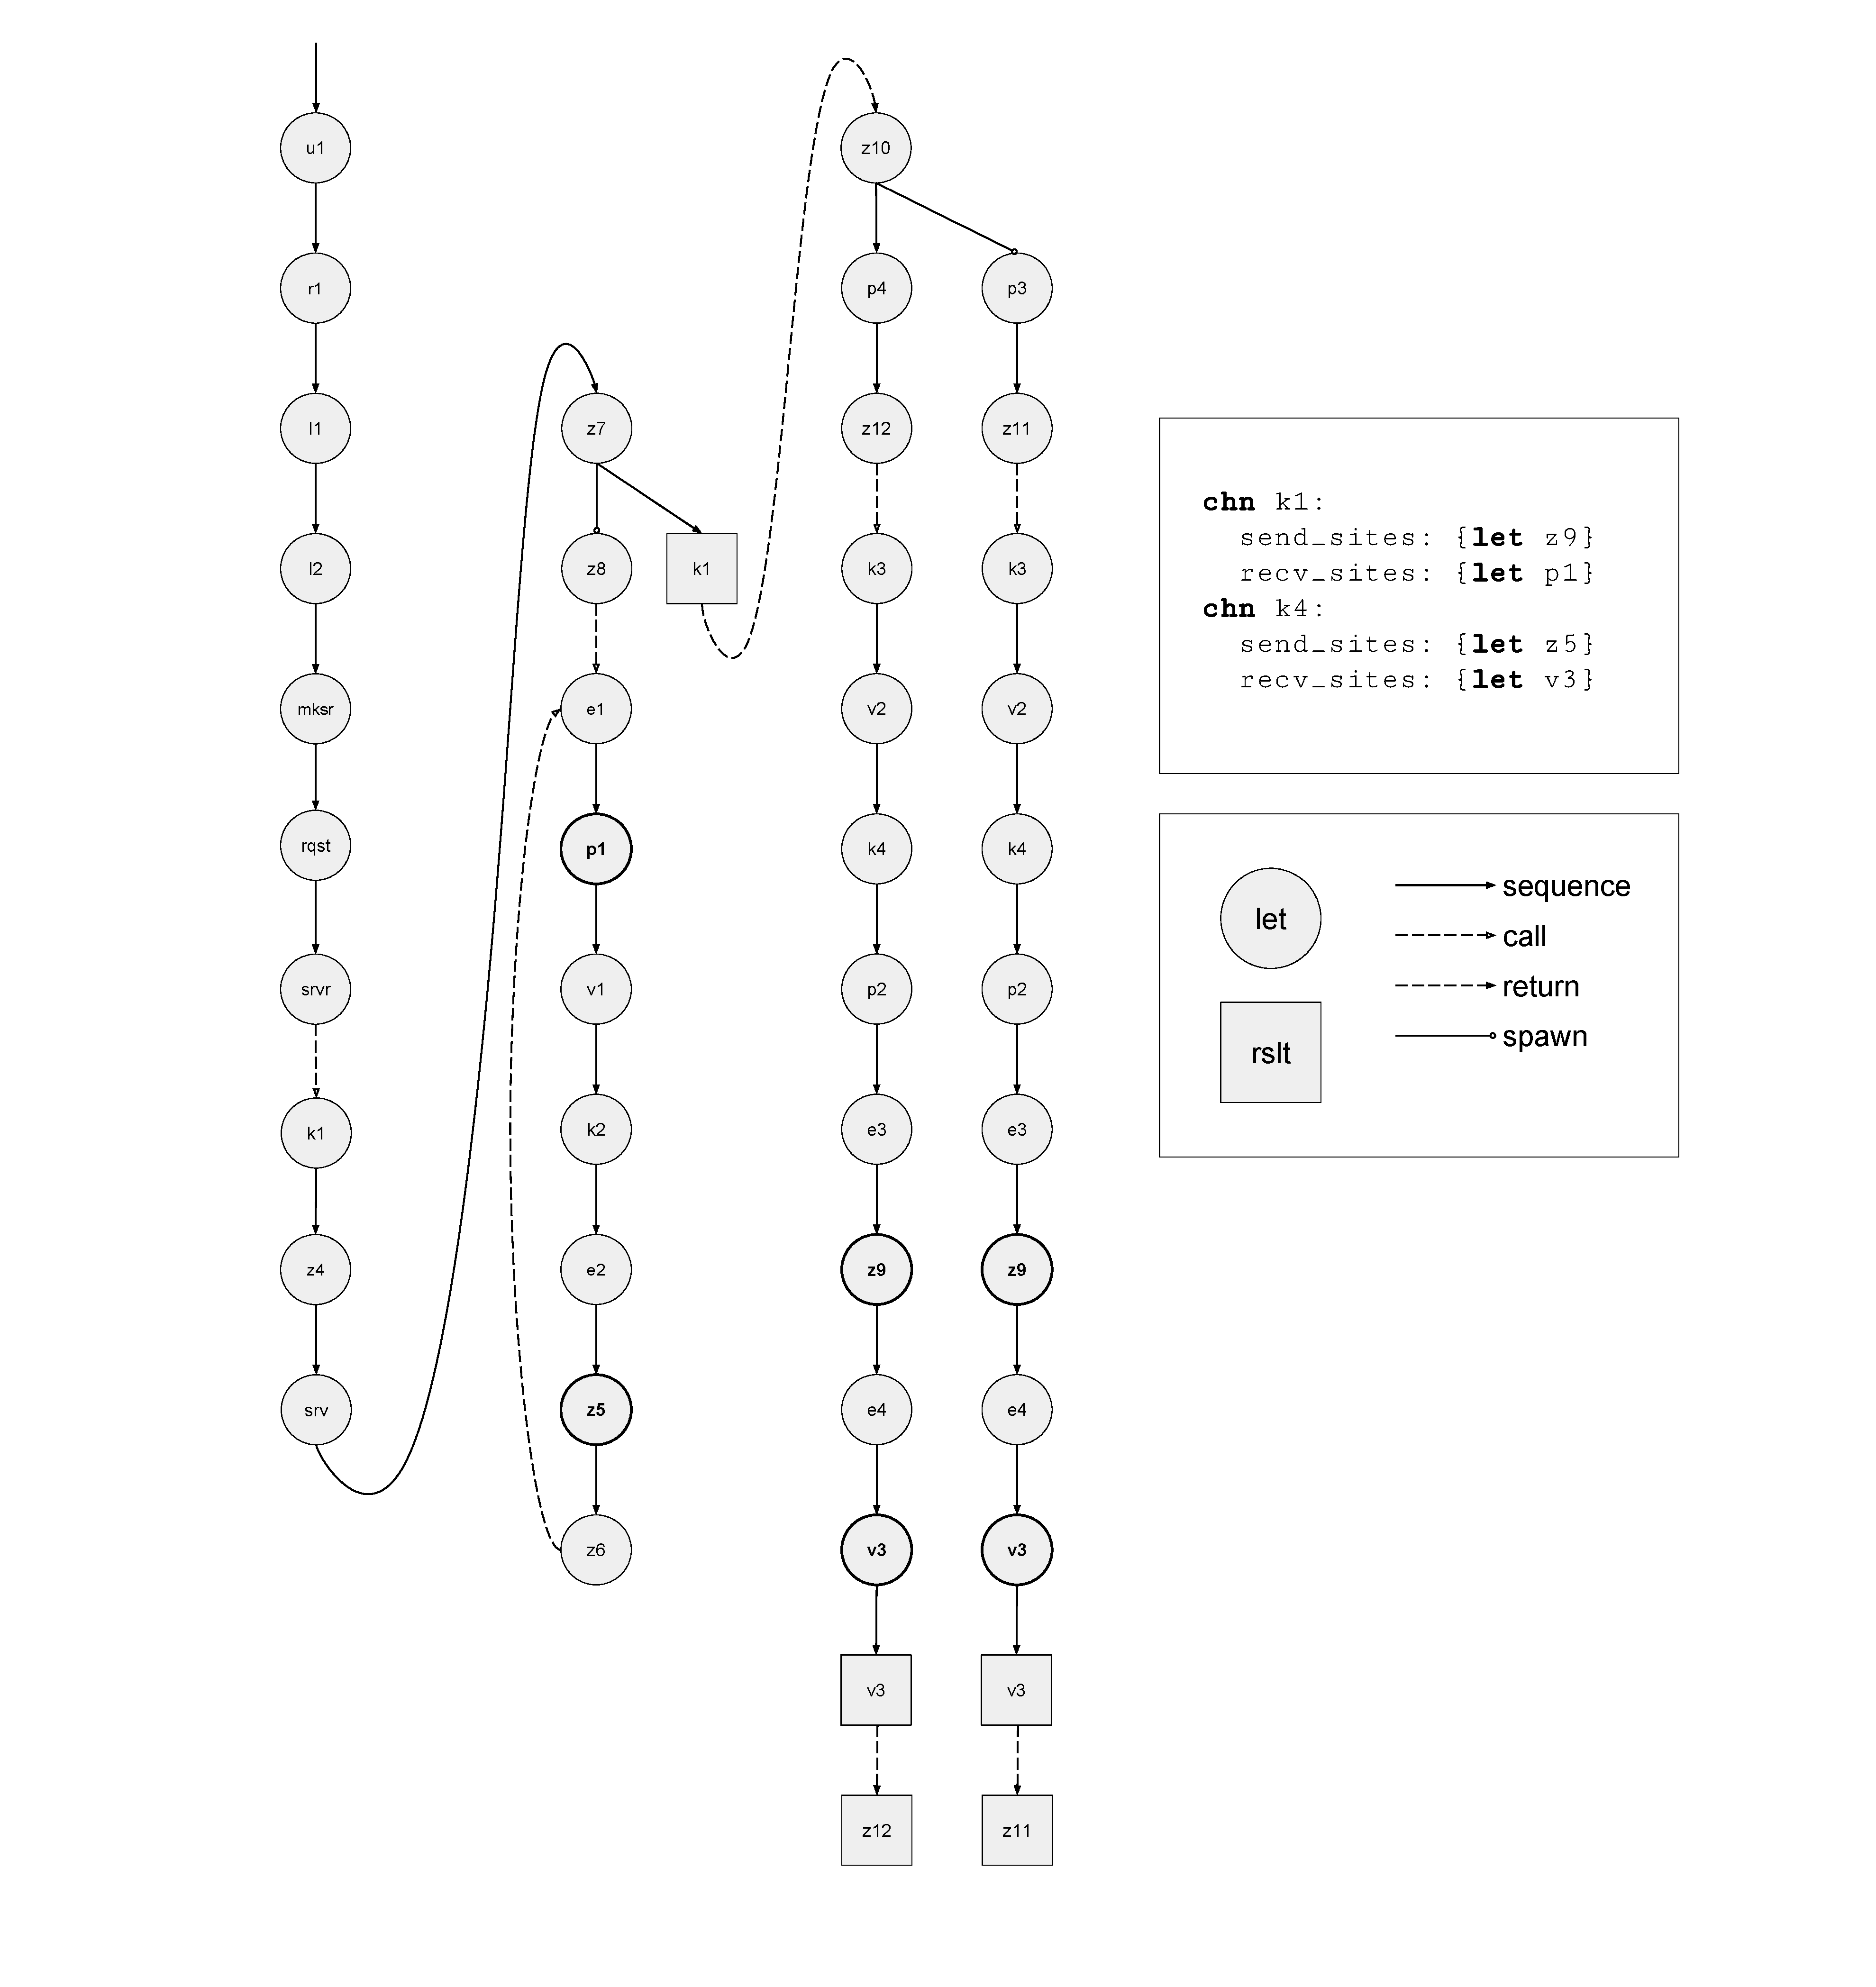
\includegraphics[width=.9\textwidth]{cml-graph.pdf}

The static traceability means that a static path with a given starting step, and ending
condition, can be traced by traversing the flows in a graph.
The empty path is statically traceable if the starting step meets the ending condition.
Otherwise, a path is statically traceable if the last static step corresponds to a flow
that meets the ending condition, and the longest strict prefix of the path is statically
traceable.  

\begin{lstlisting}[language=logic, mathescape]
  predicate staticTraceable:
    flow set -> termId -> (termId -> bool) -> static_path -> bool
  where
    empty: start graph isEnd .
      isEnd start
    $\vdash$ staticTraceable graph start isEnd []
  * snoc: graph star middle path isEnd end mode .
      staticTraceable graph start ($\lambda$ l . l = middle) path, 
      isEnd end, 
      (middle, mode, end) $\in$ graph 
    $\vdash$ staticTraceable graph start isEnd (path @ [(middle, mode)])
\end{lstlisting}

In the graph of the server implementation, there are two paths each corresponding to its
own thread that lead
to sending on
static channel \lstinline[language=sugar_lang]{chn k1} and a potentially infinite number of
paths that lead to receiving on
channel \lstinline[language=sugar_lang]{chn k1}, but all on the same thread.
There are an infinite number of paths that lead
to sending on static channel \lstinline[language=sugar_lang]{chn k4}, and two paths
that lead to receiving on static channel
\lstinline[language=sugar_lang]{chn k4}. This is certainly imprecise,
as the static \lstinline[language=sugar_lang]{chn k4} corresponds to
multiple distinct dynamic channels, each with just one sender and one receiver.  The higher
precision analysis discussed in section \ref{high-precision} addresses this issue.

The static inclusion means that two static paths might be traced in
the same run of a program. Ordered paths might be inclusive, and also a path that diverges
from another at a spawn flow might be inclusive. This concept is useful for achieving
greater precision, since if two paths cannot occur in the same run of a program, only one needs
to be counted towards the communication classification. The predicates are intended to be applied
to paths starting from the beginning of a program.

\begin{lstlisting}[language=logic, mathescape]
  predicate staticInclusive: static_path -> static_path -> bool where
    first: path1 path2 .
      prefix path1 path2
    $\vdash$ staticInclusive path1 path2
  * second path2 path1 .
      prefix path2 path1
    $\vdash$ staticInclusive path1 path2
  * spawnFirst: path n path1 path2 .
    \$vdash$ staticInclusive
      (path @ [(NBnd n, MSpwn)] @ path1)
      (path @ [(NBnd n, MNxt)] @ path2)
  * spawnSecond: path n path1 path2 .
    $\vdash$ staticInclusive
      (path @ [(NBnd n, MNxt)] @ path1])
      (path @ [(NBnd n, MSpwn)] @ path2)
\end{lstlisting}

The singularness means that two paths are the same or only of them can occur in a given run of
a program. The noncompetitiveness means states that two paths can't compete during a run of a
program, since they are ordered or cannot occur in the same run of a program.

\begin{lstlisting}[language=logic, mathescape]
  predicate singular: static_path -> static_path -> bool where
    refl: path .
    $\vdash$ singular path path
  * notInclus: path1 path2 .
      $\neg$ (staticInclusive path1 path2)
    $\vdash$ singular path1 path2

  predicate noncompetitive: static_path -> static_path -> bool where
    ordered: path1 path2 .
      ordered path1 path2
    $\vdash$ noncompetitive path1 path2
  * notInclus: path1 path2 .
      $\neg$ (staticInclusive path1 path2)
    $\vdash$ noncompetitive path1 path2
\end{lstlisting}


The static one-shot classification means that there is at most one attempt
to synchronize to send on a static channel in any run of a given program.

\begin{lstlisting}[language=logic, mathescape]
  predicate staticOneShot: static_value_map -> term -> name -> bool where
    intro: staticEnv staticComm t graph n$_c$ .
      staticEval staticEnv staticComm t,
      staticFlowsAccept staticEnv graph t,
      forEveryTwo (staticTraceable graph (termId t)
        (staticSendId staticEnv t n$_c$)) singular
    $\vdash$ staticOneShot graph t n$_c$
\end{lstlisting}

The static one-to-one classification means that there is at most one thread that attempts to
send and at most one thread that attempts to receive on a given static channel for any time
during a run of a given program.

\begin{lstlisting}[language=logic, mathescape]
  predicate staticOneToOne: static_value_map -> term -> name -> bool where
    intro: staticEnv staticComm t graph n$_c$ .
      staticEval staticEnv staticComm t,
      staticFlowsAccept staticEnv graph t,
      forEveryTwo (staticTraceable graph (termId t)
        (staticSendId staticEnv t n$_c$)) noncompetitive, 
      forEveryTwo (staticTraceable graph (termId t)
        (staticRecvId staticEnv t n$_c$)) noncompetitive
    $\vdash$ staticOneToOne staticEnv t n$_c$
\end{lstlisting}

The static one-to-many classification means that there is at most one thread that attempts to
send on a given static channel at any time during a run of a given program, but there may be
many threads that attempt to receive on the channel.

\begin{lstlisting}[language=logic, mathescape]
  predicate staticOneToMany: static_value_map -> term -> name -> bool where
    intro: staticEnv staticComm t graph n$_c$ .
      staticEval staticEnv staticComm t,
      staticFlowsAccept staticEnv graph t,
      forEveryTwo (staticTraceable graph (termId t)
        (staticSendId staticEnv t n$_c$)) noncompetitive
    $\vdash$ staticOneToMany staticEnv t n$_c$
\end{lstlisting}

The static many-to-one predicate means
that there may be many threads that attempt to send on a static channel, but there is at most
one thread that attempts to receive on the channel for any time during a run of a given
program.

\begin{lstlisting}[language=logic, mathescape]
  predicate staticManyToOne: static_value_map -> term -> name -> bool where
    intro: staticEnv statcComm t graph n$_c$ .
      staticEval staticEnv staticComm t,
      staticFlowsAccept staticEnv graph t,
      forEveryTwo (staticTraceable graph (termId t)
        (staticRecvId staticEnv t n$_c$)) noncompetitive
    $\vdash$ staticManyToOne staticEnv t n$_c$
\end{lstlisting}

\subsection{Formal Reasoning}

Reppy and Xiao informally prove soundness of their analysis by showing that their static analysis
determines that more than one thread sends (or receives) on a channel if the execution allows more
than one to send (or receive) on that channel. The proof of soundness depends on the
ability to relate the execution of a program to the static analysis of a program. The static
analysis describes threads in terms of static paths, since it can only describe threads in
terms of statically available information. Thus, in order to describe the relationship between
the threads of the static analysis and the dynamic semantics, the dynamic semantics is
defined as stepping between sets of control paths paired with terms. Divergent control paths
are added whenever a new thread is spawned.

The semantics and analysis must contain many details. To ensure the
correctness of proofs, it is necessary to check that there are no subtle errors in either the 
definitions or proofs. Proofs in general require many subtle manipulations of symbols. The
difference between a false statement and a true statement can often be difficult to spot, since
the two may be very similar lexically. However, a mechanical proof checker, such as that of 
Isabelle, has no difficulty discerning between valid and invalid derivations.
Mechanical checking of proofs can notify users of errors in the proofs or definitions far better
and faster than manual checking. This work has greatly benefited from Isabelle's proof checker in
order to correctly define the language semantics, control flow analysis, communication analysis,
and other helpful definitions. For instance, some bugs in the
definintions were found trying to prove
soundness. The proof checker would not accept the proof unless I provided facts that
should be false, indicating that the definitions did not state my intentions.
After correcting the errors in the definitions, the proof was completed such that the proof
checker was satisfied.

The reasoning involved in proving the soundness of each communication classification
is based around breaking the goal into simpler subgoals, and generalizing assumptions to create
useful induction hypotheses.  It is often useful to
create helper definitions that can be deduced
from premises of the theorem being proved and enable
general reasoning across arbitrary programs.
A frequent pattern is to define
predicates in terms of semantic structures, like the environment, stack, and pool, and deduce 
the instantiation of these predicates on the initial program state. 

Some aspects of the generalized predicate definitions exist simply to prove that they imply
instantiations of the original program based predicates. However, the generalized
definitions exist in order to allow direct access to properties that would
otherwise be deeply nested
in an inductive structure and inaccessible by a predictable number of
logical steps for an arbitrary
program.

One of the most difficult aspects of formal reasoning is in developing adequate definitions.
It is often possible to define a single semantics in multiple ways.
For instance, the sortedness of a list could be defined in terms of the sortedness of its tail
or in terms of the sortedness of its longest strict prefix. To prove theorems relating
sortedness to other relations, it may be important that the other relations are inductively
defined on the same subpart of the list. Some relations may only be definable on the tail,
while others can be defined only on the strict prefix. in such cases, it is necessary to
define sortedness in two ways, and prove their equivalence, in order to prove theorems relating
to less flexible relations.

\begin{lstlisting}[language=logic, mathescape]
  predicate sortedLeft: nat list -> bool where
    empty:
    $\vdash$ sortedRight []
  * single: x .
    $\vdash$ sortedLeft [x]
  * cons: x y zs .
      n $\leq$ y,
      sortedLeft (y # zs)
    $\vdash$ sortedLeft (x # y # zs)

  predicate sortedRight: nat list -> bool where
    empty:
    $\vdash$ sortedRight []
  * single: z .
    $\vdash$ sortedRight [z]
  * snoc: xs y z .
      sortedRight (xs @ [y]),
      y $\leq$ z 
    $\vdash$ sortedRight (xs @ [y] @ [z])

  lemma sortedEquiv: xs .
  $\vdash$ sortedLeft xs $\equiv$ sortedRight xs  
\end{lstlisting}

\subsection{Soundness}

The theorem for soundness of static one-shot classification states that if a static channel is
statically classified as one-shot for a given program and
static environment consistent with the
program, then any corresponding dynamic channel is classified
as one-shot over any pool that results
from running the program. The theorem for soundness of
static one-to-many classification states that if
a static channel is statically classified as one-to-many for a given program and static environment
consistent with that program, then any corresponding dynamic channel is classified as one-to-many
over any pool that results from running the program.  The theorems for soundness of many-to-one
classification and one-to-one classification follow the same pattern. 

\begin{lstlisting}[language=logic, mathescape]
  theorem staticOneShotSound: t$_0$ n$_c$ path$_c$ .
    staticOneShot t$_0$ n$_c$
  $\vdash$ oneShot t$_0$ (Chan path$_c$ n$_c$)

  theorem staticOneToManySound: t$_0$ n$_c$ path$_c$ . 
    staticOneToMany t$_0$ n$_c$
  $\vdash$ oneToMany t$_0$ (Chan path$_c$ n$_c$)

  theorem staticManyToOneSound: t$_0$ n$_c$ path$_c$ . 
    staticManyToOne t$_0$ n$_c$
  $\vdash$ manyToOne t$_0$ (Chan path$_c$ n$_c$)

  theorem staticOneToOneSound: t$_0$ n$_c$ path$_c$ . 
    staticOneToOne staticEnv t$_0$ n$_c$
  $\vdash$ oneToOne t$_0$ (Chan path$_c$ n$_c$)
\end{lstlisting}

The formal proofs of soundness of each static classification follow a similar structure.
Let's examine in some detail the formal proof of soudness of static one-to-many classification,
by unwinding the theorem into the lemmas that it follows from.

The following diagram illustrates the key dependencies of the theorems and lemmas in
used in the derivations.

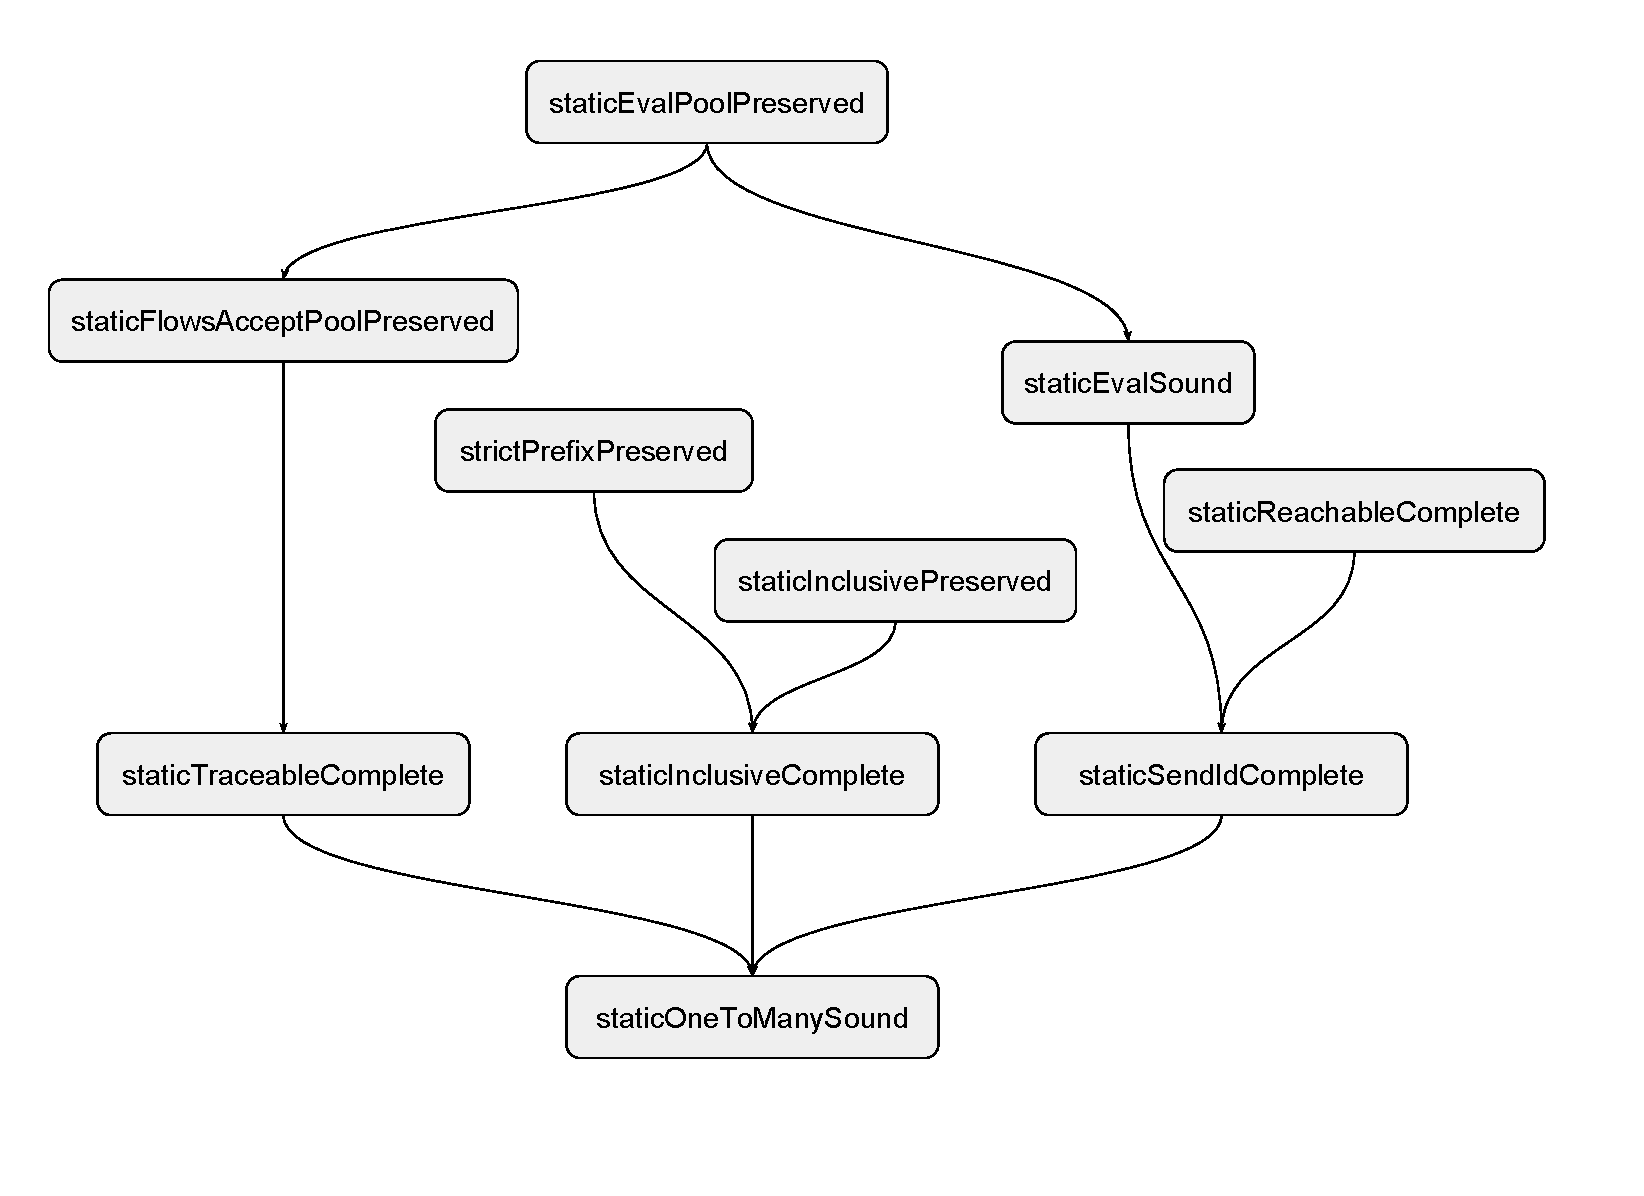
\includegraphics[width=1\textwidth]{cml-proof-low.pdf}

The soundness of static one-to-many classification is proved by a few simpler lemmas and the
definitions of static and dynamic one-to-many classification.
There is an isomorphic correspondence between the paths of
dynamic evaluation and the paths of static evaluation, by definition.
The static paths are derived from the static flow graph. Although it is possible to directly derive
the dynamic paths from the static flow graph, deriving an isomorphoic path structure keeps the the
paths relation to the static flow graph clear.  Additionally, for the higher precision analysis, static
paths are not isomorphic to dynamic paths. 

The three main lemmas state the
soundness of the static traceability, the soundness of the static inclusiveness, and
the soundness of a program step not being a static sending identifier. These lemmas depend on a
correspondence between static paths and dynamic paths, which is bijective for the lower
precision analysis. The lemma for soundness of static inclusiveness states that any two
dynamic paths traced by running a program correspond to statically inclusive static paths. It
follows from a straightforward case analysis of static inclusivity. The lemma for soundness of
static traceability states that for any dynamic path traced by running a program, there
is a corresponding static path that is statically traceable. The lemma for soundness of a
program step not being a static sending identifier states that running a program reaches a
synchronization on a sending event, then that synchronization is statically identified as a
sending identifier by its term identifier.


\begin{lstlisting}[language=logic, mathescape]
  predicate pathsCorrespond: dynamic_path -> static_path -> bool where
    empty:
    $\vdash$ pathsCorrespond [] []
  * seq: path staticPath n .
      pathsCorrespond path staticPath
    $\vdash$ pathsCorrespond
      (path @ [DNxt n])
      (staticPath @ [(NBnd n, MNxt)])
  * spawn: path staticPath n .
      pathsCorrespond path staticPath
    $\vdash$ pathsCorrespond
      (path @ [DSpwn n])
      (staticPath @ [(NBnd n, MSpwn)])
  * call: path staticPath n .
      pathsCorrespond path staticPath
    $\vdash$ pathsCorrespond
      (path @ [DCll n])
      (staticPath @ [(NBnd n, MCll)])
  * return: path staticPath n .
      pathsCorrespond path staticPath
    $\vdash$ pathsCorrespond
      (path @ [DRtn n])
      (staticPath @ [(NRslt n, MRtn)])

  lemma staticTraceableSound: t$_0$ pool comm path n c t' env stack staticEnv staticComm graph isEnd .
    star dynamicEval ([[] -> (Stt t$_0$ [->] [])], {}) (pool, comm), 
    pool path = Some (Stt (Bind n c t') env stack),
    staticEval staticEnv staticComm t$_0$,
    staticFlowsAccept staticEnv graph t$_0$,
    isEnd (NBnd n)
  $\vdash$ exists staticPath . 
    pathsCorrespond path staticPath
  $\wedge$ staticTraceable graph (termId t$_0$) isEnd staticPath

  lemma staticInclusiveSound: t$_0$ pool comm path1 stt1 path2 stt2 staticPath1 staticPath2 . 
    star dynamicEval [[] -> (Stt t$_0$ [->] [])] {} pool comm
    pool path1 = Some stt1, 
    pool path2 = Some stt2, 
    pathsCorrespond path1 staticPath1, 
    pathsCorrespond path2 staticPath2
  $\vdash$ staticInclusive staticPath1 staticPath2

  lemma staticSendIdSound: t$_0$ pool comm path n n$_e$ t' env stack n$_{sc}$ n$_m$ env' path$_c$ n$_c$ .
    star dynamicEval [[] -> (Stt t$_0$ [->] [])] {} pool comm, 
    pool path = Some (Stt (Bind n (Sync n$_e$) t') env stack), 
    env n$_e$ = Some (VAtm (SendEvt n$_{sc}$ n$_m$) env'), 
    env' n$_{sc}$ = Some (VChn (Chan path$_c$ n$_c$)), 
    staticEval staticEnv staticComm t$_0$
  $\vdash$ staticSendId staticEnv t$_0$ n$_c$ (NBnd n)
\end{lstlisting}

The completeness of static traceability is proved by generalizing
static acceptance by flows and static evaluation over pools, such that information about a step in
the program can be deduced by a fixed number of logical steps regardless of the location of the
program step or the size of the program. Without such generalization, it would be possible to
prove soundness for a fixed program, but not any arbitrary program.

The generalization of static acceptance by flows is comprised of static acceptance by flows over values,
static acceptance by flows over environments, static acceptance by flows over stacks, and static
acceptance by flows over pools.
In most cases, it simply states that an embedded term of some semantic element is also statically
accepting. The exception is in the case of
static acceptance by flows over a non-empty stack, where
there is an additional condition that the flow
from a result identifier to the term identifier
of the continuation program exists in the graph.
This information is consistent with static
acceptance by flows over programs, but provides direct information about a flow in the
graph, which would otherwise only be deducible by a varying number of logical steps
depending on the program.

\begin{lstlisting}[language=logic, mathescape]
  predicate staticFlowsAcceptValue:
    static_value_map -> graph -> dynamic_value -> bool
  where
    unit: staticEnv graph .
    $\vdash$ staticFlowsAcceptValue staticEnv graph VUnt
  * chan: staticEnv graph n$_c$ .
    $\vdash$ staticFlowsAcceptValue staticEnv graph (VChn n$_c$)
  * sendEvt: staticEnv graph env n$_c$ n$_m$.
      staticFlowsAcceptEnv staticEnv graph env 
    $\vdash$ staticFlowsAcceptVal
      staticEnv graph (VAtm (SendEvt n$_c$ n$_m$) env)
  * recvEvt: staticEnv graph env n$_c$.
      staticFlowsAcceptEnv staticEnv graph env 
    $\vdash$ staticFlowsAcceptVal
      staticEnv graph (VAtm (RecvEvt n$_c$) env)
  * left: staticEnv graph env n$_p$ .
      staticFlowsAcceptEnv staticEnv graph env 
    $\vdash$ staticFlowsAcceptVal
      staticEnv graph (VAtm (Lft n$_p$) env)
  * right: staticEnv graph env n$_p$ .
      staticFlowsAcceptEnv staticEnv graph env
    $\vdash$ staticFlowsAcceptVal
        staticEnv graph (VAtm (Rht n$_p$) env)
  * function: staticEnv graph t$_b$ env n$_f$ n$_p$ .
      staticFlowsAccept staticEnv graph t$_b$, 
      staticFlowsAcceptEnv staticEnv graph env
    $\vdash$ staticFlowsAcceptVal
        staticEnv graph (VAtm (Fun n$_f$ n$_p$ t$_b$) env)
  * pair: staticEnv graph env . 
      staticFlowsAcceptEnv staticEnv graph env
    $\vdash$ staticFlowsAcceptVal
      staticEnv graph (VAtm (Pair n$_1$ n$_2$) env)

  predicate staticFlowsAcceptEnv:
    static_value_map -> graph -> env -> bool
  where 
    intro: staticEnv graph env .
      $\forall$ n v . 
        env n = Some v
      $\rightarrow$ staticFlowsAcceptValue staticEnv graph v
    $\vdash$ staticFlowsAcceptEnv staticEnv graph env

  predicate staticFlowsAcceptStack:
    static_value_map -> graph -> name -> stack -> bool
  where
    empty: staticEnv graph n$_r$ .
    $\vdash$ staticFlowsAcceptStack staticEnv graph n$_r$ []
  * cons: n$_r$ t graph staticEnv graph env stack n env .
      {(NRslt y, MRtn, termId t)} $\subseteq$ graph,
      staticFlowsAccept staticEnv graph t,
      staticFlowsAcceptEnv staticEnv graph env,
      staticFlowsAcceptStack staticEnv graph (resultName t) stack 
    $\vdash$ staticFlowsAcceptStack staticEnv graph n$_r$ ((Ctn n t env) # stack)

  predicate staticFlowsAcceptPool of
    static_value_map -> graph -> pool -> bool
  where
    intro: staticEnv graph pool .
      $\forall$ path t env stack .
        env path = Some (Stt t env stack)
      $\rightarrow$
        staticFlowsAccept staticEnv graph t
      $\wedge$ staticFlowsAcceptEnv staticEnv graph env
      $\wedge$ staticFlowsAcceptStack staticEnv graph (resultName t) stack
    $\vdash$ staticFlowsAcceptPool staticEnv graph pool
\end{lstlisting}

The flows described by the various versions of static acceptance by flows depend on static
environments in order to look up the control flow in the case where the term is a function.
The static environment
results from the static evaluation of the program that is dynamically evaluated. Thus,
generalized
versions of static evaluation enable further deduction about flows.
As with the generalized versions of static acceptance by flows,
the generalized versions of static evaluation are designed to
preserve static environments across
dynamic evaluations of pools. They also provide direct access to binding information from names
to static values in a fixed number of logical steps. Static evaluation of programs correlates
program syntax to static values, but the generalized static evaluations correlate dynamic
semantic structures, like, value, environments, and stacks, to static values. The function
relates dynamic values to static values and helps the larger goal of relating dynamic
semantic elements to static values and static environments.    

\begin{lstlisting}[language=logic, mathescape]
  fun abstract: dynamic_value -> static_value where
    $\vdash$ abstract VUnt = SUnt
  * path n . 
    $\vdash$ abstract (VChn (Chan path x)) = SChn x
  * atom env .
    $\vdash$ abstract (VAtm atom env) = SAtm atom

  predicate staticEvalValue:
    static_value_map -> static_value_map -> dynamic_value -> bool
  where
    unit: staticEnv staticComm .
    $\vdash$  staticEvalValue staticEnv staticComm VUnit)
  * chan: staticEnv staticComm c .
    $\vdash$ staticEvalValue staticEnv staticComm (VChn c))
  * sendEvt: staticEnv staticComm env n$_c$ n$_m$ .
      staticEvalEnv staticEnv staticComm env
    $\vdash$ staticEvalValue staticEnv staticComm
      (VAtm (SendEvt n$_c$ n$_m$) env))
  * recvEvt: staticEnv staticComm env n$_c$  .
      staticEvalEnv staticEnv staticComm env
    $\vdash$ staticEvalValue staticEnv staticComm
      (VAtm (RecvEvt n$_c$) env))
  * left: staticEnv staticComm env n$_p$  .
      staticEvalEnv staticEnv staticComm env
    $\vdash$ staticEvalValue staticEnv staticComm
      (VAtm (Lft n$_p$) env))
  * right: staticEnv staticComm env n$_p$  .
      staticEvalEnv staticEnv staticComm env
    $\vdash$ staticEvalValue staticEnv staticComm
      (VAtm (Rht n$_p$) env))
  * function: n$_f$ n$_p$ t$_b$ staticEnv staticComm env .
      {SAtm (Fun n$_f$ n$_p$ t$_b$)} $\subseteq$ staticEnv f, 
      staticEval staticEnv staticComm t$_b$, 
      staticEvalEnv staticEnv staticComm env
    $\vdash$ staticEvalValue staticEnv staticComm
      (VAtm (Fun n$_f$ n$_p$ t$_b$) env))
  * pair: staticEnv staticComm env n$_1$ n$_2$ .
      staticEvalEnv staticEnv staticComm env
    $\vdash$ staticEvalValue staticEnv staticComm
      (VAtm (Pair n$_1$ n$_2$) env))

  predicate staticEvalEnv:
    static_value_map -> static_value_map -> env -> bool
  where 
    intro: staticEnv staticComm env .
      $\forall$ n v .
        env n = Some v 
      $\rightarrow$ {abstract v} $\subseteq$ staticEnv n
      $\wedge$ staticEvalValue staticEnv staticComm v
    $\vdash$ staticEvalEnv staticEnv staticComm env

  predicate staticEvalStack:
    static_value_map -> static_value_map 
  -> static_value set -> stack -> bool 
  where
    empty: staticEnv staticComm staticVals .
    $\vdash$ staticEvalStack staticEnv staticComm staticVals [])
  * cons: staticVals staticEnv staticComm . 
      staticVals $\subseteq$ staticEnv n,
      staticEval staticEnv staticComm t,
      staticEvalEnv staticEnv staticComm env,
      staticEvalStack staticEnv staticComm (staticEnv (resultName t)) stack 
    $\vdash$ staticEvalStack staticEnv staticComm staticVals ((Ctn n t env) # stack))

  predicate staticEvalPool:
    static_value_map -> static_value_map -> pool -> bool
  where
    intro: staticEnv staticComm pool .
      $\forall$ path t env stack .
        pool path = Some (Stt t env stack)
      $\rightarrow$ 
        staticEval staticEnv staticComm t
      $\wedge$ staticEvalEnv staticEnv staticComm env
      $\wedge$ staticEvalStack staticEnv staticComm (staticEnv (resultName t)) stack)
    $\vdash$ staticEvalPool staticEnv staticComm pool)
  \end{lstlisting}


A variant of star that inducts toward the left of the transitive connection is helpful for
relating dynamic traceability to static traceability, since it mirrors the direction that way
paths grow, which influenced the choice of induction in the definition of static
traceability.

\begin{lstlisting}[language=logic, mathescape]
  predicate starLeft: ('a -> 'a -> bool) -> 'a -> 'a -> bool where
    refl: r z z .
    $\vdash$ starLeft r z z
  * trans: r x y z .
      starLeft r x y,
      r y z
    $\vdash$ starLeft r x z

  lemma starImpliesStarLeft: r x z .
    star r x z
  $\vdash$ starLeft r x z

  lemma starLeftTrans: r x y z .
    starLeft r x y,
    starLeft r y z 
  $\vdash$ starLeft r x z
\end{lstlisting}

The lemma for the completeness of static traceability follows from the generalized definitions
of static acceptance by flows, the definition of static traceability, and the preservation
of static acceptance by flows across multiples steps of evaluation.

\begin{lstlisting}[language=logic, mathescape]
  lemma staticFlowsAcceptPoolPreserved: t$_0$ pool comm staticEnv staticComm graph .
    star dynamicEval [[] -> (Stt t$_0$ [->] [])] {} pool comm, 
    staticEval staticEnv staticComm t$_0$,
    staticFlowsAcceptPool staticEnv graph [[] -> (Stt t$_0$ [->] [])]
  $\vdash$ staticFlowsAcceptPool staticEnv graph pool 
\end{lstlisting}

The preservation of static acceptance by flows over pools is proved by the
equivalence between star and its leftward variant, and induction on the leftward variant.
The preservation of static evalatuation of pools over multiple steps is also relied upon.

\begin{lstlisting}[language=logic, mathescape]
  lemma staticEvalPoolPreserved: pool comm pool' comm' staticEnv staticComm .
    star dynamicEval pool comm pool' comm' 
    staticEvalPool staticEnv staticComm pool
  $\vdash$ staticEvalPool staticEnv staticComm pool'
\end{lstlisting}

The completeness of static inclusiveness is derived from various lemmas that
preserve relations from pairs of dynamic paths to pairs of corresponding static paths.  
Some of these, among many others, are
the preservation of the strict prefix relation from static to dynamic paths,
and the preservation of static inclusiveness over extension of static paths.

\begin{lstlisting}[language=logic, mathescape]
  lemma strictPrefixPreservedCorresp: staticPathath1 staticPath2 dynamicPath1 dynamicPath2 .
    strictPrefix staticPathath1 staticPath2, 
    pathsCorrespond dynamicPath1 staticPath1,
    pathsCorrespond dynamicPath2 staticPath2
  $\vdash$ strictPrefix dynamicPath1 dynamicPath2

  lemma staticInclusivePreservedUnorderedExtension: path1 path2 l1 l2 .
    staticInclusive path1 path2, 
    $\neg$ (prefix path1 path2),
    $\neg$ (prefix path2 path1), 
  $\vdash$ staticInclusive (path1 @ [l1]) (path2 @ [l2])
\end{lstlisting}

These various preservation lemmas are derived from the basic properites of lists 
and straight forward properities of path correspondence, such as commutitivity, as
well as foundational principles like induction of corresponding paths.

The lemma for completeness of sending identifier classification \lstinline{staticSendIdSound}
is proved using the lemma for
soundness of static evaluation for synchronization of a send event,
and the lemma for soundness of static evaluation.
Since only sending identifiers are relevant the completeness of static reachability is
used to ensure that the static step is indeed a sending identifier. 

\begin{lstlisting}[language=logic, mathescape]
  lemma sendChanStaticEvalSound: t$_0$ pool comm staticEnv staticComm path
  n n$_e$ t' env stack n$_{sc}$ n$_m$ env$_e$ path$_c$ n$_c$ .
    star dynamicEval [[] -> (Stt t$_0$ [->] [])] {} pool comm,
    staticEval staticEnv staticComm t$_0$,
    pool path = Some (Stt (Bind n (Sync n$_e$) t') env stack),
    env n$_e$ = Some (VAtm (SendEvt n$_{sc}$ n$_m$) env$_e$),
    env$_e$ n$_{sc}$ = Some (VChn (Chan path$_c$ n$_c$))
  $\vdash$ SChn n$_c$ $\in$ staticEnv n$_{sc}$

  lemma staticEvalSound: t$_0$ pool comm staticEnv staticComm path t env stack n v .
    staticEval staticEnv staticComm t$_0$, 
    star dynamicEval [[] -> (Stt t$_0$ [->] [])] {} pool comm,
    pool path = Some (Stt t env stack), 
    env n = Some v
  $\vdash$ abstract v $\in$ staticEnv n 

  lemma staticReachableSound: t$_0$ pool comm staticEnv staticComm path t env stack .
    star dynamicEval [[] -> (Stt t$_0$ [->] [])] {} pool comm,
    pool path = Some (Stt t env stack)
  $\vdash$ staticReachable t$_0$ t 
\end{lstlisting}

Both the soundness of static evaluation on the syncrhonization of a send event,
and the soundness of static evaluation follow from
the preservation of static evaluation over multiple steps of dynamic evaluation.

The lemma for completeness of static reachability relies on a reformulation of
static reachability defined by proofs that induct on a larger term
containing the reachable term.  This definition is useful for forward derivations
of reachability relations, however it doesn't offer much guidance for deciding reachability. 
In constrast, the definition of the original static reachability relation is
syntax-directed in order to portray a clear connection to
a computable algorithm that can determine the reachable term from an initial program.
To show that an term is reachable from the initial program, it is necessary to
show that each intermediate term is reachable from the initial term.  Thus, the
induction needs to enable unraveling the goals from the end of the program to the beginning,
maintaining the initial program state in context for each subgoal. Because the static
reachable relation is a "may", the generalized relations should hold unless there is
a clear reason that it could never hold. For instance, in the relation over atoms, it holds
for all atoms other than functions, it holds without any additional demands. 

\begin{lstlisting}[language=logic, mathescape]
  predicate staticReachableForward: term -> term -> bool where
    refl: t$_0$ .
    $\vdash$ staticReachableForward t$_0$ t$_0$
  * spawn: t$_0$ n t$_c$ t' .
      staticReachableForward t$_0$ (Bind n (Spwn t$_c$) t')
    $\vdash$ staticReachableForward t$_0$ t$_c$
  * caseLeft: t$_0$ n n$_s$ n$_l$ t$_l$ n$_r$ t$_r$ t' .
      staticReachableForward t$_0$ (Bind n (Case n$_s$ n$_l$ t$_l$ n$_r$ t$_r$) t')
    $\vdash$ staticReachableForward t$_0$ t$_l$
  * caseRight: t$_0$ n n$_s$ n$_l$ t$_l$ n$_r$ t$_r$ t' .
      staticReachableForward t$_0$ (Bind n (Case n$_s$ n$_l$ t$_l$ n$_r$ t$_r$) t')
    $\vdash$ staticReachableForward t$_0$ t$_r$
  * function: t$_0$ n n$_f$ n$_p$ t$_b$ t' .
      staticReachableForward t$_0$ (Bind n (Atom (Fun n$_f$ n$_p$ t$_b$)) t')
    $\vdash$ staticReachableForward t$_0$ t$_b$
  * seq: t$_0$ n n$_f$ n$_p$ t$_b$ t' .
      staticReachableForward t$_0$ (Bind n c t')
    $\vdash$ staticReachableForward t$_0$ t'

  predicate staticReachableAtom: term -> atom -> bool where
    sendEvt: t$_0$ n$_c$ n$_m$ .
    $\vdash$ staticReachableAtom t$_0$ (SendEvt n$_c$ n$_m$)
  * recvEvt: t$_0$ n$_c$ .
    $\vdash$ staticReachableAtom t$_0$ (RecvEvt n$_c$)
  * pair: t$_0$ n$_1$ n$_2$ .
    $\vdash$ staticReachableAtom t$_0$ (Pair n$_1$ n$_2$)
  * left: t$_0$ n$_l$ .
    $\vdash$ staticReachableAtom t$_0$ (Lft n$_l$)
  * right: t$_0$ n$_r$
    $\vdash$ staticReachableAtom t$_0$ (Rht n$_r$)
  * function: t$_0$ t$_b$ n$_f$ n$_p$ t$_b$ . 
      staticReachableForward t$_0$ t$_b$ 
    $\vdash$ staticReachableAtom t$_0$ (Fun n$_f$ n$_p$ t$_b$)

  predicate staticReachableVal: term -> dynamic_value -> bool where
    unit: t$_0$ .
    $\vdash$ staticReachableValue t$_0$ VUnt
  * chan: t$_0$ c .
    $\vdash$ staticReachableValue t$_0$ (VChn c)
  * atom: t$_0$ t env .
      staticReachableAtom t$_0$ t, 
      staticReachableEnv t$_0$ env
    $\vdash$ staticReachableValue t$_0$ (VAtm t env)

  predicate staticReachableEnv: term -> env -> bool where
    intro: t$_0$ env
      $\forall$ n v . 
        env n = Some v
      $\rightarrow$ staticReachableValue t$_0$ v
    $\vdash$ staticReachableEnv t$_0$ env

  predicate staticReachableStack: term -> stack -> bool where
    empty: t$_0$ .
    $\vdash$ staticReachableStack t$_0$ [])
  * cons: t$_0$ t$_k$ env$_k$ stack' .
      staticReachableForward t$_0$ t$_k$, 
      staticReachableEnv t$_0$ env$_k$,
      staticReachableStack t$_0$ stack' 
    $\vdash$ staticReachableStack t$_0$ ((Ctn n$_k$ t$_k$ env$_k$) # stack')

  predicate staticReachablePool: term -> pool -> bool where
    intro: t$_0$ pool .
      $\forall$ path t env stack .
        pool path = Some (Stt t env stack) 
      $\rightarrow$ staticReachableForward t$_0$ t
      $\wedge$ staticReachableEnv t$_0$ env
      $\wedge$ staticReachableStack t$_0$ stack
    $\vdash$ staticReachablePool t$_0$ pool

\end{lstlisting}

The completeness of static reachability follows the definitions
a generalized form of completeness over pools.

\begin{lstlisting}[language=logic, mathescape]
  lemma staticReachablePoolSound: t$_0$ pool .
    star dynamicEval [[] -> (Stt t$_0$ [->] [])], {} pool comm 
  $\vdash$ staticReachablePool t$_0$ pool
\end{lstlisting}

The completeness over pools follows from the lemma that the forward
static reachability implies the rightward (and syntax-directed) static reachability,
and the equivalence between star and the forward star.  It relies on induction of the
forward star and constructs the static reachability
proposition using the forward definition.  

\begin{lstlisting}[language=logic, mathescape]
  lemma staticReachableForwardImpliesStaticReachable: t$_0$ t. 
    staticReachableForward t$_0$ t
  $\vdash$ staticReachable t$_0$ t

  lemma staticReachableTrans: t1 t2 t3 .
    staticReachable t1 t2,
    staticReachable t2 t3
  $\vdash$ staticReachable t1 t3
\end{lstlisting}

The lemma that the forward variant of static reachability implies the syntax-directed static
reachability follows from induction on the forward static reachability and the
transitivity of static reachability, which follows from induction on static reachability.

\section{Higher Precision Communication} \label{high-precision}
In many programs, like in the server example, channels are created within s.
The s may be applied multiple times, creating multiple distinct channels
with each application. It may be that each channel is used just once and then discarded.
However, the static analysis just described would identify all the distinct channels by the
same name, since each distinct channel is created by the same piece of syntax.
Thus, it would classify those channels as being used more than once.

It is possible to be more precise by trimming the program under analysis down to just the part
where the static channel is live. The static channel cannot be live between the last use of a
dynamic channel and the creation of a new dynamic channel with the same name.  Thus, each
truncated program would have just one dynamic channel corresponding to the static channel under
analysis. 

The higher precision analysis uses a trimmed down graph to better differentiate between distinct channels. 
A trimmed graph is specialized for a particular dynamic channel.  From the creation
step, it must contain transitive flows to all the program steps where the
channel is live. It should also be as small as possible, for higher precision.

In the whole graph used in the previous analysis, a spawning flow
connects a child thread to the rest of the program.  For a trimmed graph,
it may be clear the channel of interest is not created until after the spawn step,
so there is not need to include the spawning flow.  However, later on in the
program it may become apparent that the channel of interest is sent via another channel to
that spawned thread.  Since there is no spawning flow already connecting that
thread to the trimmed graph, a flow with a sending mode is used between the
sending identifier and the receiving identifier of synchronization.
Modes for typical control flow of
sequencing, calling, returning, and spawning are also included flows.

\begin{lstlisting}[language=logic, mathescape]
  datatype mode =
    MNxt
  | MSpwn
  | ESend name
  | MCll
  | MRtn

  type flow = termId * mode * termId

  type static_step = termId * mode

  type staticPath = static_step list
\end{lstlisting}

We use a slightly modified version of the server implementation
to demonstrate some key concepts of the higher precision analysis.
An additional loop function \lstinline{lp} has been added to the
server implementation. The loop basically just wastes steps, but it is used to demontrate how
liveness analysis treats functions that don't contain any channel of interest.

\begin{lstlisting}[language=normal_lang, mathescape]
  bind u1 = unt
  bind r1 = rht u1
  bind l1 = lft r1
  bind l2 = lft l1

  bind lp = fun lp' x1 => 
  (
    bind z1 = case x1 of 
      lft y1 =>
      (
        bind z2 = app lp' y1
        rslt z2
      )
    | rht y2 =>
      (
        bind u2 = unt
        rslt u2
      )
    bind u3 = unt
    rslt u3
  )

  bind mksr = fun _ x2 => 
  (
    bind k1 = mkChn
    bind z4 = lp l2
    bind srv = fun srv' x3 =>
    (
      bind e1 = recvEvt k1
      bind p1 = sync e1
      bind v1 = fst p1
      bind k2 = snd p1 
      bind e2 = sendEvt k2 x3
      bind z5 = sync e2
      bind z6 = app srv' v1
      rslt z6 
    )
    bind z7 = spawn
    (
      bind z8 = srv r1
      rslt z8
    )
    rslt k1
  )

  bind rqst = fun _ x4 =>
  (
    bind k3 = fst x4
    bind v2 = snd x4
    bind k4 = mkChn
    bind p2 = pair v2 k4
    bind e3 = sendEvt k3 p2
    bind z9 = sync e3
    bind e4 = recvEvt k4
    bind v3 = sync e4
    rslt v3
  )

  bind srvr = mksr u1
  bind z10 = spawn
  ( 
    bind p3 = pair srvr l1
    bind z11 = app rqst p3
    rslt z11
  )
  bind p4 = pair srvr l2
  bind z12 = app rqst p4
  rslt z12
\end{lstlisting}


The static acceptance by flows for higher precision is similar to that of the lower precision analysis.
However, it must additionally consider flows with the sending mode. 

\begin{lstlisting}[language=logic, mathescape]
  predicate staticFlowsAcceptTm:
    static_value_map -> graph -> term -> term -> bool
  where
    result: staticEnv graph n .
    $\vdash$ staticFlowsAcceptTm staticEnv graph t$_0$ (Rslt n)
  * unit: n t' graph staticEnv .
      (NBnd n , MNxt, termId t') $\in$ graph,
      staticFlowsAcceptTm staticEnv graph t$_0$ t'
    $\vdash$ staticFlowsAcceptTm staticEnv graph t$_0$ (Bind n Unt t')
  * makeChan: n t' graph staticEnv  .
      (NBnd n , MNxt, termId t') $\in$ graph,
      staticFlowsAcceptTm staticEnv graph t$_0$ t'
    $\vdash$ staticFlowsAcceptTm staticEnv graph t$_0$ (Bind n MkChn t')
  * sendEvt: n t' graph staticEnv  n$_c$ n$_m$ .
      (NBnd n , MNxt, termId t') $\in$ graph,
      staticFlowsAcceptTm staticEnv graph t$_0$ t'
    $\vdash$ staticFlowsAccept
      staticEnv graph
      (Bind n (Atom (SendEvt n$_c$ n$_m$)) t')
  * recvEvt: n t' graph staticEnv n$_c$ .
      (NBnd n , MNxt, termId t') $\in$ graph,
      staticFlowsAcceptTm staticEnv graph t$_0$ t'
    $\vdash$ staticFlowsAcceptTm staticEnv graph t$_0$ (Bind n (Atom (RecvEvt n$_c$)) t')
  * pair: n t' graph staticEnv n$_1$ n$_2$ .
      (NBnd n , MNxt, termId t') $\in$ graph,
      staticFlowsAcceptTm staticEnv graph t$_0$ t'
    $\vdash$ staticFlowsAcceptTm staticEnv graph t$_0$ (Bind n (Atom (Pair n$_1$ n$_2$)) t')
  * left: n t' graph staticEnv n$_s$ .
      (NBnd n , MNxt, termId t') $\in$ graph,
      staticFlowsAcceptTm staticEnv graph t$_0$ t'
    $\vdash$ staticFlowsAcceptTm staticEnv graph t$_0$ (Bind n (Atom (Lft n$_s$)) t')
  * right: n t' graph staticEnv n$_s$ .
      (NBnd n , MNxt, termId t') $\in$ graph,
      staticFlowsAcceptTm staticEnv graph t$_0$ t'
    $\vdash$ staticFlowsAcceptTm staticEnv graph t$_0$ (Bind n (Atom (Rht n$_s$)) t')
  * function: n t' graph staticEnv t$_b$ n$_f$ n$_p$ .
      (NBnd n , MNxt, termId t') $\in$ graph,
      staticFlowsAcceptTm staticEnv graph t$_0$ t',
      staticFlowsAcceptTm staticEnv graph t$_0$ t$_b$
    $\vdash$ staticFlowsAcceptTm staticEnv graph t$_0$ (Bind n (Atom (Fun n$_f$ n$_p$ t$_b$)) t')
  * spawn: n t' t$_c$ graph staticEnv.
      {(NBnd n, MNxt, termId t'),
        (NBnd n, MSpwn, termId t$_c$)} $\subseteq$ graph,
      staticFlowsAcceptTm staticEnv graph t$_0$ t$_c$,
      staticFlowsAcceptTm staticEnv graph t$_0$ t'
    $\vdash$ staticFlowsAcceptTm staticEnv graph t$_0$ (Bind n (Spwn t$_c$) t')
  * sync: n t' graph staticEnv n$_{se}$ .
      (NBnd n , MNxt, termId t') $\in$ graph,
      $\forall$ n$_{sc}$ n$_m$ n$_c$ n$_y$.
        (SAtm (SendEvt n$_{sc}$ n$_m$)) $\in$ staticEnv nSE,
      $\rightarrow$ (SChn n$_c$) $\in$ staticEnv n$_{sc}$
      $\rightarrow$ staticRecvId staticEnv t$_0$ n$_c$ (NBnd n$_y$)
      $\rightarrow$ (NBnd n, ESend n$_{se}$, NBnd n$_y$) $\in$ graph),
      staticFlowsAcceptTm staticEnv graph t$_0$ t'
    $\vdash$ staticFlowsAcceptTm staticEnv graph t$_0$ (Bind n (Sync n$_{se}$) t')
  * first: n t' graph staticEnv n$_p$ .
      (NBnd n , MNxt, termId t') $\in$ graph,
      staticFlowsAcceptTm staticEnv graph t$_0$ t',
    $\vdash$ staticFlowsAcceptTm staticEnv graph t$_0$ (Bind n (Fst n$_p$) t')
  * second: n t' graph staticEnv n$_p$ .
      (NBnd n , MNxt, termId t') $\in$ graph,
      staticFlowsAcceptTm staticEnv graph t$_0$ t',
    $\vdash$ staticFlowsAcceptTm staticEnv graph t$_0$ (Bind n (Snd n$_p$) t')
  * caseEither: n t$_l$ t$_r$ t' graph staticEnv n$_s$ .
      {
        (NBnd n, MCll, termId t$_l$),
        (NBnd n, MCll, termId t$_r$),
        (NRslt (resultName t$_l$), MRtn, termId t'),
        (NRslt (resultName t$_r$), MRtn, termId t')
      } $\subseteq$ graph,
      staticFlowsAcceptTm staticEnv graph t$_0$ t$_l$,
      staticFlowsAcceptTm staticEnv graph t$_0$ t$_r$,
      staticFlowsAcceptTm staticEnv graph t$_0$ t'
    $\vdash$ staticFlowsAcceptTm staticEnv graph t$_0$ (Bind n (Case n$_s$ n$_l$ t$_l$ n$_r$ t$_r$) t')
  * app: staticEnv n$_f$ n t' n n$_a$ .
      $\forall$ n$_f$' n$_p$ t$_b$ . 
        (SAtm (Fun n$_f$' n$_p$ t$_b$)) $\in$ staticEnv n$_f$
      $\rightarrow$
        {
          (NBnd n, MCll, termId t$_b$),
          (NRslt (resultName t$_b$), MRtn, termId t')
        } $\subseteq$ graph),
      staticFlowsAcceptTm staticEnv graph t$_0$ t'
    $\vdash$ staticFlowsAcceptTm staticEnv graph t$_0$ (Bind n (App n$_f$ n$_a$) t')

  predicate staticFlowsAccept:
    static_value_map -> graph -> term -> bool
  where
    intro: staticEnv graph n .
      staticFlowsAcceptTm staticEnv graph t$_0$ t$_0$
    $\vdash$ staticFlowsAccept staticEnv graph t$_0$ 

\end{lstlisting}

The server implementation represented as a graph illustrates how static acceptance by
flows can interpret a program as a flow graph.

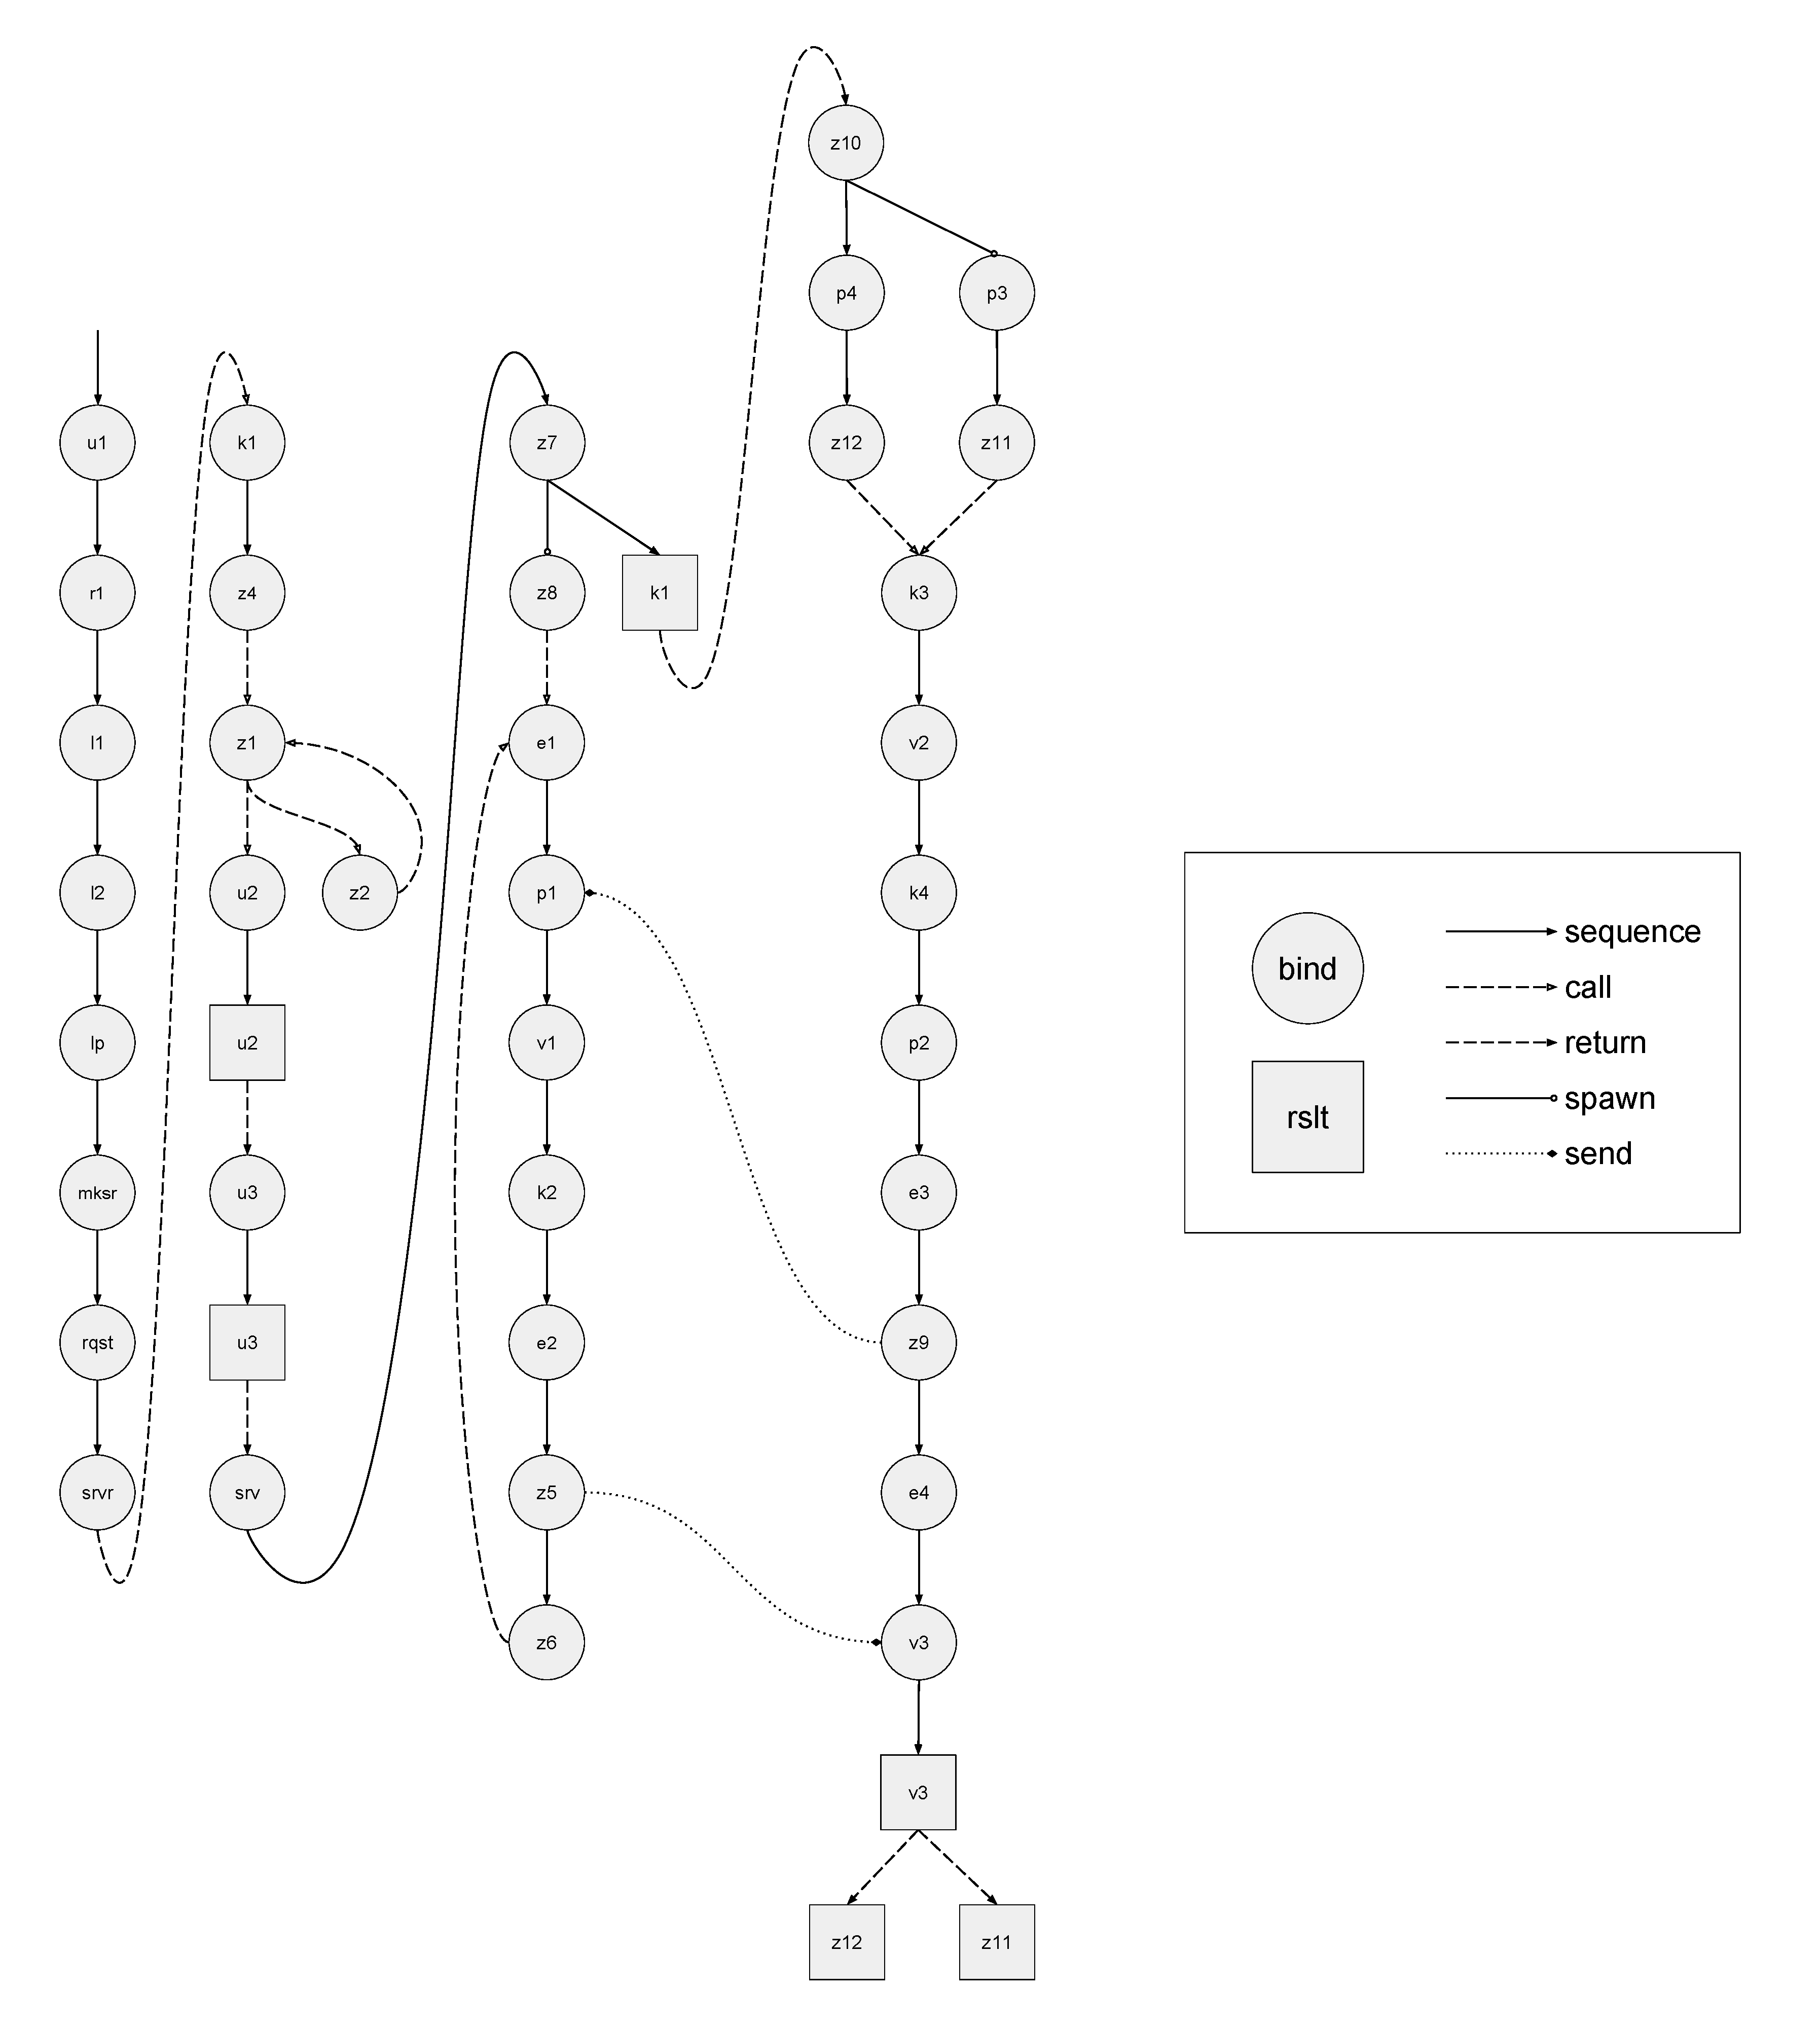
\includegraphics[width=1\textwidth]{cml-graph-lp.pdf}


For the liveness of channel analysis, it is necessary to track any name built on a channel.
A name is build on a channel if the name binds to a static value 
containing a channel of interest, or a static value that contains names built on the channel.
In the case where the tracked name possibly binds to a function,
for the name to be considered built on a channel,
the channel simply needs to be live in the body of the function.
This condition is represented formally as the requirement that there is a 
name, such that it is a free variable in the function, and it's built on the channel.

\begin{lstlisting}[language=logic, mathescape]

  fun freeVarsAtom: atom -> name set where
    n$_c$ n$_m$ .
    $\vdash$ freeVarsAtom (SendEvt n$_c$ n$_m$) = {n$_c$, n$_m$}
  * n$_c$ .
      freeVarsAtom (RecvEvt n$_c$) = {n$_c$}
  * n$_1$ n$_2$ .
    $\vdash$ freeVarsAtom (Pair n$_1$ n$_2$) = {n$_1$, n$_2$}
  * n .
    $\vdash$ freeVarsAtom (Lft n) = {n}
  * n .
    $\vdash$ freeVarsAtom (Rht n) = {n}
  * n$_f$ n$_p$ t$_b$ .
    $\vdash$ freeVarsAtom (Fun n$_f$ n$_p$ t$_b$) = freeVarsTerm t$_b$ \ {n$_f$, n$_p$}
  
  and freeVarsComplex: complex -> name set where
    $\vdash$ freeVarsComplex Unt = {}
  * $\vdash$ freeVarsComplex MkChn = {}
  * atom .
    $\vdash$ freeVarsComplex (Atom atom) = freeVarsAtom atom
  * t .
    $\vdash$ freeVarsComplex (Spwn t) = freeVarsTerm t
  * n .
    $\vdash$ freeVarsComplex (Sync n) = {n}
  * n .
    $\vdash$ freeVarsComplex (Fst n) = {n}
  * n .
    $\vdash$ freeVarsComplex (Snd n) = {n},

  * n$_s$ n$_l$ t$_l$ n$_r$ t$_r$ .
    $\vdash$ freeVarsComplex (Case n$_s$ n$_l$ t$_l$ n$_r$ t$_r$) = 
      {n$_s$} $\cup$ freeVarsTerm t$_l$ $\cup$ freeVarsTerm t$_r$ \ {n$_l$, n$_r$}
  * n$_f$ n$_a$ .
    $\vdash$ freeVarsComplex (App n$_f$ n$_a$) = {n$_f$, n$_a$},
  
  and freeVarsTerm: term -> name set where
    n c t .
    $\vdash$ freeVarsTerm (Bind n c t) = freeVarsComplex c $\cup$ freeVarsTerm t \ {n}
  * n .
    $\vdash$ freeVarsTerm (Rslt n) = {n}

  predicate staticBuiltOnChan: static_value_map -> name -> name -> bool where
    chan: n$_c$ staticEnv n .
      SChn n$_c$ $\in$ staticEnv n 
    $\vdash$ staticBuiltOnChan staticEnv n$_c$ n
  * sendEvt: n$_{sc}$ n$_m$ staticEnv n n$_c$ . 
      (SAtm (SendEvt n$_{sc}$ n$_m$)) $\in$ staticEnv n,
      (
        staticBuiltOnChan staticEnv n$_c$ n$_{sc}$ 
      $\vee$ staticBuiltOnChan staticEnv n$_c$ n$_m$
      )
    $\vdash$ staticBuiltOnChan staticEnv n$_c$ n
  * recvEvt: n$_{rc}$ staticEnv n n$_c$ . 
      (SAtm (RecvEvt n$_{rc}$)) $\in$ staticEnv n,
      staticBuiltOnChan staticEnv n$_c$ n$_{rc}$
    $\vdash$ staticBuiltOnChan staticEnv n$_c$ n
  * pair: n$_1$ n$_2$ staticEnv n n$_c$ . 
      (SAtm (Pair n$_1$ n$_2$)) $\in$ staticEnv n,
      (
        staticBuiltOnChan staticEnv n$_c$ n$_1$ 
      $\vee$ staticBuiltOnChan staticEnv n$_c$ n$_2$
      )
    $\vdash$ staticBuiltOnChan staticEnv n$_c$ n
  * left: n$_a$ staticEnv n n$_c$ .
      (SAtm (Lft n$_a$)) $\in$ staticEnv n,
      staticBuiltOnChan staticEnv n$_c$ n$_a$
    $\vdash$ staticBuiltOnChan staticEnv n$_c$ n
  * right: n$_a$ staticEnv n n$_c$ .
      (SAtm (Rht n$_a$)) $\in$ staticEnv n,
      staticBuiltOnChan staticEnv n$_c$ n$_a$
    $\vdash$ staticBuiltOnChan staticEnv n$_c$ n
  * function: n$_f$ n$_p$ t$_b$ n$_{fv}$ .
      (SAtm (Fun n$_f$ n$_p$ t$_b$)) $\in$ staticEnv n,
      n$_{fv}$ $\in$ freeVarsAtom (Fun n$_f$ n$_p$ t$_b$),
      staticBuiltOnChan staticEnv n$_{fv}$ n
    $\vdash$ staticBuiltOnChan staticEnv n$_c$ n
\end{lstlisting}


The static liveness of a channel describes entry functions and exit functions.
The entry function maps a term identifier to a set of names built on
the given channel, if those names are live at the entry of that term identifier.
The exit function maps a term identifier to a
set of names built on the given channel, if those names are live at the exit of that
term identifier.

The following diagram illustrates the entry and exit sets of each term id
for channel \lstinline{k1} in
the server example.  Each entry set appears right above its related term identifier,
and each exit setappears right below its related term identifier. 

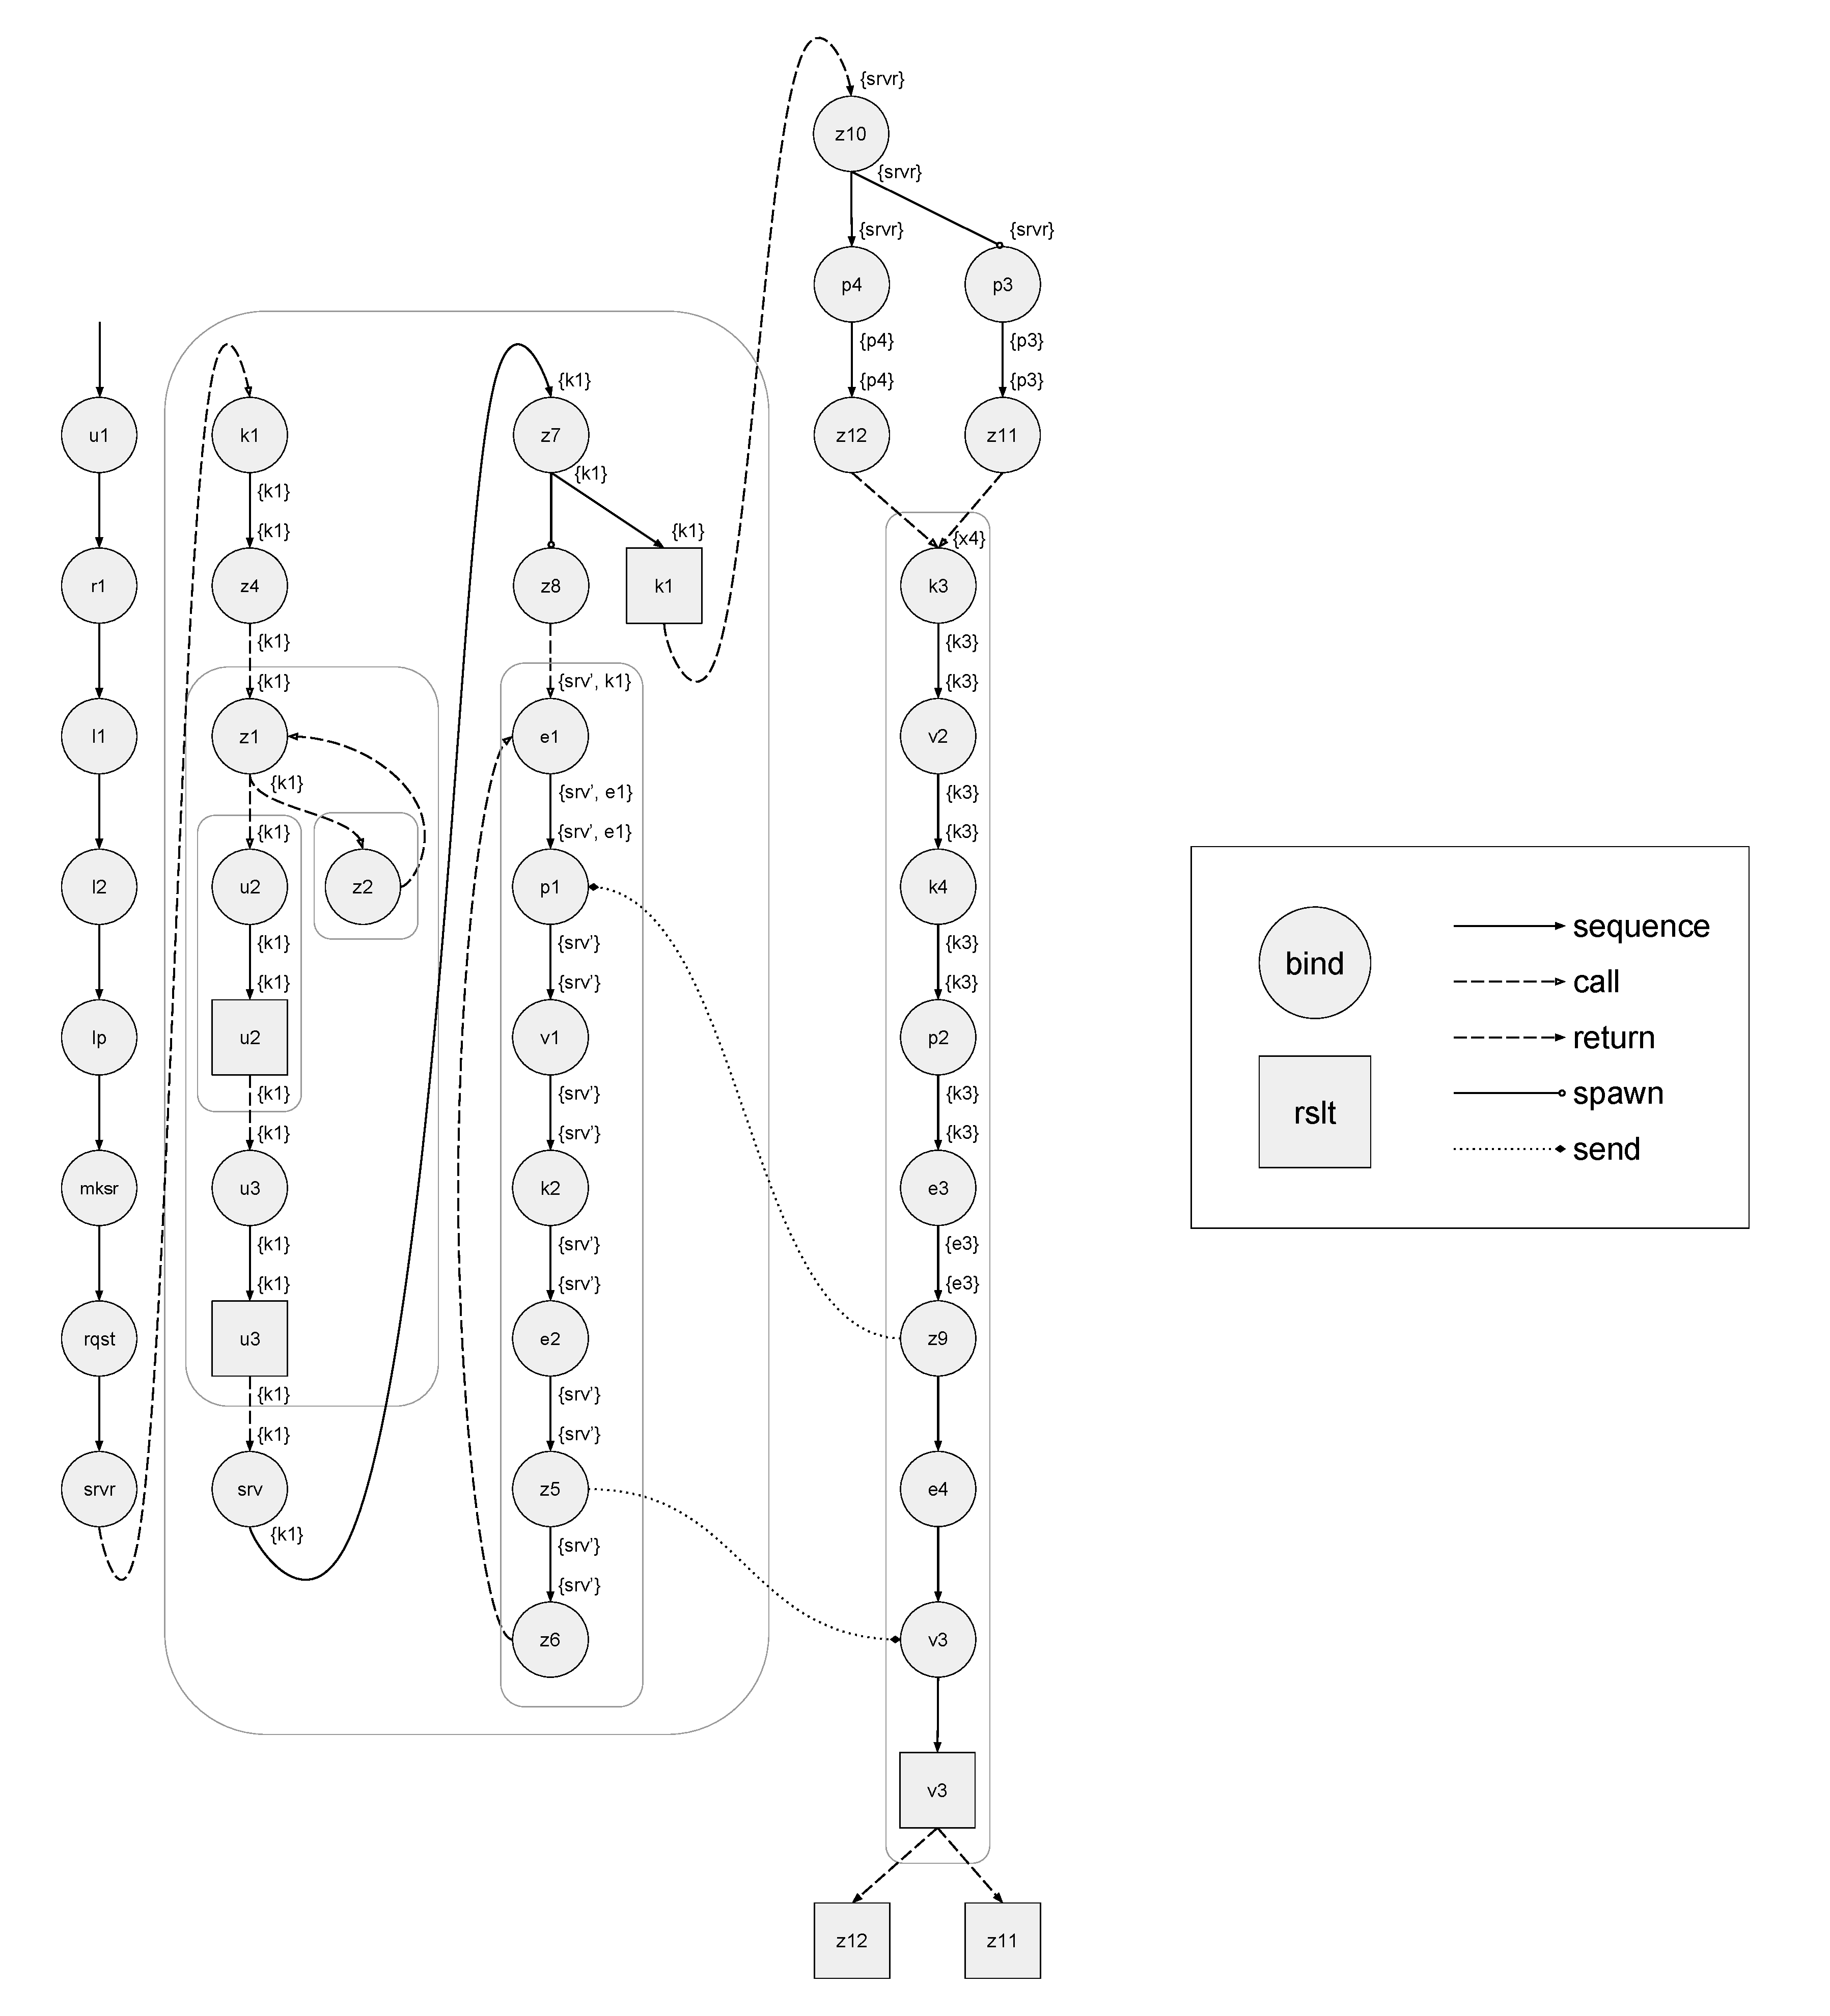
\includegraphics[width=1\textwidth]{cml-liveness-analysis-k1.pdf}

The following diagram illustrates the entry and exit sets of each term id
for channel \lstinline{k4} in
the server example.  Each entry set appears right above its related term identifier,
and each exit setappears right below its related term identifier. 

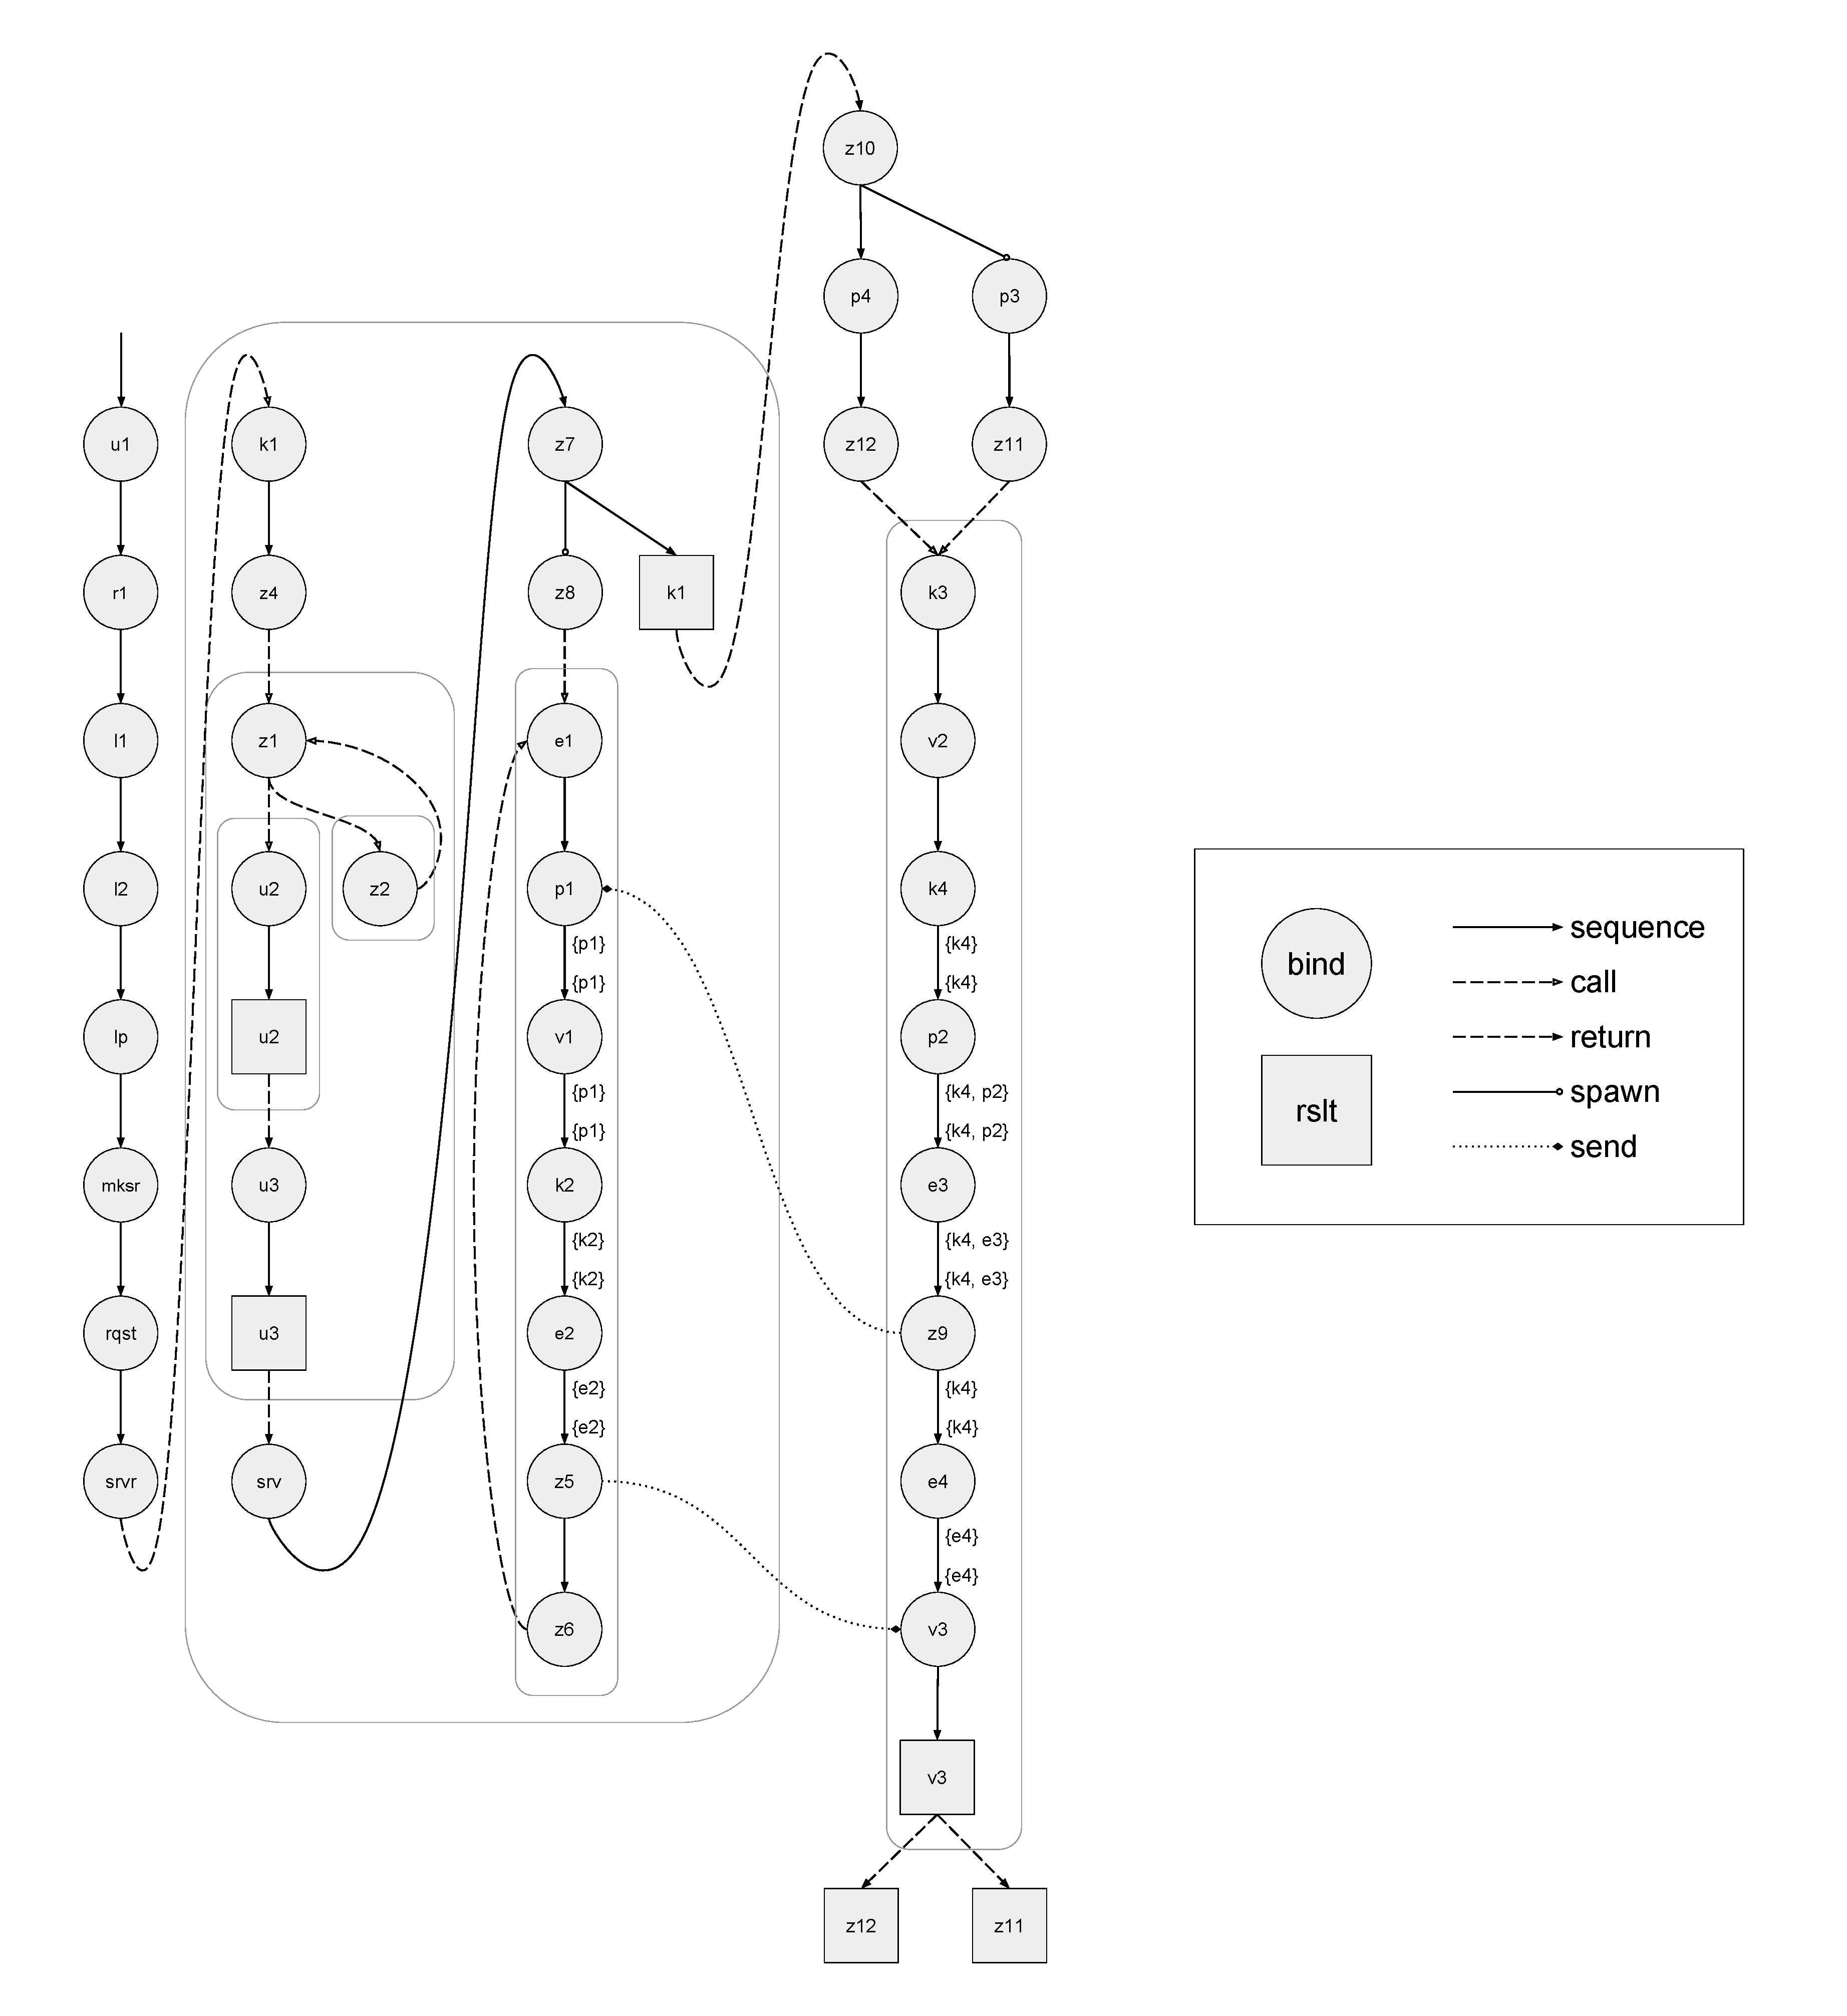
\includegraphics[width=1\textwidth]{cml-liveness-analysis-k4.pdf}

\begin{lstlisting}[language=logic, mathescape]
  predicate staticLiveChan:
    static_value_map -> term_id_map 
  -> term_id_map -> name -> term -> bool
  where
    result: staticEnv entr n$_c$ n$_y$ exit .
      (
        (staticBuiltOnChan staticEnv n$_c$ n$_y$)
      $\rightarrow$ {n$_y$} $\subseteq$ entr (NRslt n$_y$)
      )
    $\vdash$ staticLiveChan staticEnv entr exit n$_c$ (Rslt n$_y$)
  * unit: exit n entr t' staticEnv n$_c$ .
      (exit (NBnd n) \ {n}) $\subseteq$ entr (NBnd n),
      entr (termId t') $\subseteq$ exit (NBnd n),
      staticLiveChan staticEnv entr exit n$_c$ t'
    $\vdash$ staticLiveChan staticEnv entr exit n$_c$ (Bind n Unt t')
  * makeChan: exit n entr t' staticEnv n$_c$ .
      (exit (NBnd n) \ {n}) $\subseteq$ entr (NBnd n),
      entr (termId t') $\subseteq$ exit (NBnd n),
      staticLiveChan staticEnv entr exit n$_c$ t'
    $\vdash$ staticLiveChan staticEnv entr exit n$_c$ (Bind n MkChn t')
  * sendEvt: exit n entr staticEnv n$_c$ n$_{sc}$ n$_m$ t' n$_c$ .
      (exit (NBnd n) \ {n}) $\subseteq$ entr (NBnd n),
      (staticBuiltOnChan staticEnv n$_c$ n$_{sc}$
      $\rightarrow$ {n$_{sc}$} $\subseteq$ entr (NBnd n)),
      (staticBuiltOnChan staticEnv n$_c$ n$_m$
      $\rightarrow$ {n$_m$} $\subseteq$ entr (NBnd n)),
      entr (termId t') $\subseteq$ exit (NBnd n),
      staticLiveChan staticEnv entr exit n$_c$ t'
    $\vdash$ staticLiveChan staticEnv entr exit n$_c$
      (Bind n (Atom (SendEvt n$_{sc}$ n$_m$)) t')
  * recvEvt: exit n entr staticEnv n$_c$ n$_r$ n$_{rc}$.    
      (exit (NBnd n) \ {n}) $\subseteq$ entr (NBnd n),
      (staticBuiltOnChan staticEnv n$_c$ n$_r$ then
      $\rightarrow$ {n$_r$} $\subseteq$ entr (NBnd n)),
      entr (termId t') $\subseteq$ exit (NBnd n),
      staticLiveChan staticEnv entr exit n$_c$ t'
    $\vdash$ staticLiveChan staticEnv entr exit n$_c$
      (Bind n (Atom (RecvEvt n$_{rc}$)) t')
  * pair: exit n entr staticEnv t$_c$ n$_1$ n$_2$ t' .
      (exit (NBnd n) \ {n}) $\subseteq$ entr (NBnd n),
      (staticBuiltOnChan staticEnv n$_c$ n$_1$
      $\rightarrow$ {n$_1$} $\subseteq$ entr (NBnd n)),
      (staticBuiltOnChan staticEnv n$_c$ n$_2$
      $\rightarrow$ {n$_2$} $\subseteq$ entr (NBnd n)),
      entr (termId t') $\subseteq$ exit (NBnd n),
      staticLiveChan staticEnv entr exit n$_c$ t'
    $\vdash$ staticLiveChan staticEnv entr exit n$_c$ (Bind n (Atom (Pair n$_1$ n$_2$)) t'))
  * left: exit n entr staticEnv n$_c$ n$_a$ t' . 
      (exit (NBnd n) \ {n}) $\subseteq$ entr (NBnd n),
      (staticBuiltOnChan staticEnv n$_c$ n$_a$
      $\rightarrow$ {n$_a$} $\subseteq$ entr (NBnd n)),
      entr (termId t') $\subseteq$ exit (NBnd n),
      staticLiveChan staticEnv entr exit n$_c$ t'
    $\vdash$ staticLiveChan staticEnv entr exit n$_c$ (Bind n (Atom (Lft n$_a$)) t'))
  * right: exit n entr staticEnv n$_c$ n$_a$ t' . 
      (exit (NBnd n) \ {n}) $\subseteq$ entr (NBnd n),
      (staticBuiltOnChan staticEnv n$_c$ n$_a$
      $\rightarrow$ {n$_a$} $\subseteq$ entr (NBnd n))
      entr (termId e) $\subseteq$ exit (NBnd n),
      staticLiveChan staticEnv entr exit n$_c$ t
    $\vdash$ staticLiveChan staticEnv entr exit n$_c$ (Bind n (Atom (Rht n$_a$)) e)
  * function: exit n entr t$_b$ n$_p$ n staticEnv n$_c$ t' n$_f$ . 
      (exit (NBnd n) \ {n}) $\subseteq$ entr (NBnd n),
      (entr (termId t$_b$) \ {n$_f$, n$_p$}) $\subseteq$ entr (NBnd n),
      staticLiveChan staticEnv entr exit n$_c$ t$_b$,
      entr (termId t') $\subseteq$ exit (NBnd n),
      staticLiveChan staticEnv entr exit n$_c$ t'
    $\vdash$ staticLiveChan staticEnv entr exit n$_c$
      (Bind n (Atom (Fun n$_f$ n$_p$ t$_b$)) t')
  * spawn: exit n entr t' t$_c$ n$_c$ staticEnv .
      (exit (NBnd n) \ {n}) $\subseteq$ entr (NBnd n),
      entr (termId t') $\subseteq$ exit (NBnd n),
      entr (termId t$_c$) $\subseteq$ exit (NBnd n),
      staticLiveChan staticEnv entr exit n$_c$ t$_c$,
      staticLiveChan staticEnv entr exit n$_c$ t'
    $\vdash$ staticLiveChan staticEnv entr exit n$_c$
      (Bind n (Spwn t$_c$) t')
  * sync: exit n entr staticEnv n$_c$ n$_e$ t' .
      (exit (NBnd n) \ {n}) $\subseteq$ entr (NBnd n),
      (staticBuiltOnChan staticEnv n$_c$ n$_e$
       $\rightarrow$ {n$_e$} $\subseteq$ entr (NBnd n)),
      entr (termId t') $\subseteq$ exit (NBnd n),
      staticLiveChan staticEnv entr exit n$_c$ t',
    $\vdash$ staticLiveChan staticEnv entr exit n$_c$
      (Bind n (Sync n$_e$) t')
  * first: exit n entr staticEnv n$_c$ n$_a$ t' .
      (exit (NBnd n) \ {n}) $\subseteq$ entr (NBnd n),
      (staticBuiltOnChan staticEnv n$_c$ n$_a$
      $\rightarrow$ {n$_a$} $\subseteq$ entr (NBnd n)),
      entr (termId t') $\subseteq$ exit (NBnd n),
      staticLiveChan staticEnv entr exit n$_c$ t'
    $\vdash$ staticLiveChan staticEnv entr exit n$_c$ (Bind n (Fst n$_a$) t')
  * $\forall$ exit n entr staticEnv n$_c$ n$_a$ t' .
      (exit (NBnd n) \ {n}) $\subseteq$ entr (NBnd n),
      (staticBuiltOnChan staticEnv n$_c$ n$_a$ then
      $\rightarrow$ {n$_a$} $\subseteq$ entr (NBnd n)),
      entr (termId t') $\subseteq$ exit (NBnd n),
      staticLiveChan staticEnv entr exit n$_c$ t'
    $\vdash$ staticLiveChan staticEnv entr exit n$_c$
      (Bind n (Snd n$_a$) t')
  * caseEither: exit n entr t$_l$ n$_l$ t$_r$ n$_r$ staticEnv n$_c$ n$_s$ t' .
      (exit (NBnd n) \ {n}) $\subseteq$ entr (NBnd n),
      (entr (termId t$_l$) \ {n$_l$}) $\subseteq$ entr (NBnd n),
      (entr (termId t$_r$) \ {n$_r$}) $\subseteq$ entr (NBnd n),
      (staticBuiltOnChan staticEnv n$_c$ n$_s$
      $\rightarrow$ {n$_s$} $\subseteq$ entr (NBnd n)),
      staticLiveChan staticEnv entr exit n$_c$ t$_l$,
      staticLiveChan staticEnv entr exit n$_c$ t$_r$,
      entr (termId t') $\subseteq$ exit (NBnd n),
      staticLiveChan staticEnv entr exit n$_c$ t'
    $\vdash$ staticLiveChan staticEnv entr exit n$_c$ (Bind n (Case n$_s$ n$_l$ t$_l$ n$_r$ t$_r$) t')
  * app: exit n entr staticEnv n$_c$ n$_a$ n$_f$ t' .
      (exit (NBnd n) \ {n}) $\subseteq$ entr (NBnd n),
      (staticBuiltOnChan staticEnv n$_c$ n$_a$
      $\rightarrow$ {n$_a$} $\subseteq$ entr (NBnd n)),
      (staticBuiltOnChan staticEnv n$_c$ n$_f$
      $\rightarrow$ {n$_f$} $\subseteq$ entr (NBnd n)),
      entr (termId t') $\subseteq$ exit (NBnd n),
      staticLiveChan staticEnv entr exit n$_c$ t'
    $\rightarrow$ staticLiveChan staticEnv entr exit n$_c$ (Bind n (App n$_f$ n$_a$) t')
\end{lstlisting}

The static liveness of a flow checks if a flow exists in a whole graph,
and if it meets certain criteria with respect to the entry and exit liveness
functions.  The channel liveness relation says if a channel is live within a function, but
does not say anything whether or not a channel remains live across calling or returning flows.
The liveness of flows can check if the liveness is mainted across function bounardies, in addition
to simply lifting the static liveness the analysis for the intraprocedural flows.
No channel is considered to be live in the body of the loop at \lstinline[language=normal_lang]{bind lp}.
However, a channel may be live before the loop is
called and after the loop returns. In such a case, the live flow is retained
from the caller to within the loop function's body, even though the steps in
the loop may not be live according to the entry function in the static channel liveness.

\begin{lstlisting}[language=logic, mathescape]
  predicate staticLiveFlow:
    graph -> term_id_map -> term_id_map -> flow -> bool where
    $\forall$ l l' graph exit entr . 
      if
        (l, MNxt, l') $\in$ graph,
        not (exit l = {}),
        not (entr l' = {})
      then
        staticLiveFlow graph entr exit (l, MNxt, l')
  * $\forall$ l l' graph exit entr .
      if
        (l, MSpwn, l') $\in$ graph, 
        not (exit l = {}),
        not (entr l' = {})
      then
        staticLiveFlow graph entr exit (l, MSpwn, l')
  * $\forall$ l l' graph exit entr .
      if
        (l, MCll, l') $\in$ graph,
        (not (exit l = {})) $\vee$ (not (entr l' = {}))
      then
        staticLiveFlow graph entr exit (l, MCll, l')
  * $\forall$ l l' graph entr exit .
      if
        (l, MRtn, l') $\in$ graph,
        not (entr l' = {})
      then
        staticLiveFlow graph entr exit (l, MRtn, l')
  * $\forall$ n$_s$ n$_e$ n$_r$ graph entr exit .
      if
        ((NBnd n$_s$), ESend n$_e$, (NBnd n$_r$)) $\in$ graph, 
        {n$_e$} $\subseteq$ (entr (NBnd n$_s$))
      then
        staticLiveFlow graph entr exit
        ((NBnd n$_s$), ESend n$_e$, (NBnd n$_r$))
\end{lstlisting}

The static traceability for the higher precision analysis states
that an entire static path can be traced through some graph and
is live with respect to some entry and exit functions.

The following diagram illustrates the graph of the server example,
containing only live flows for channel \lstinline{k1}. \

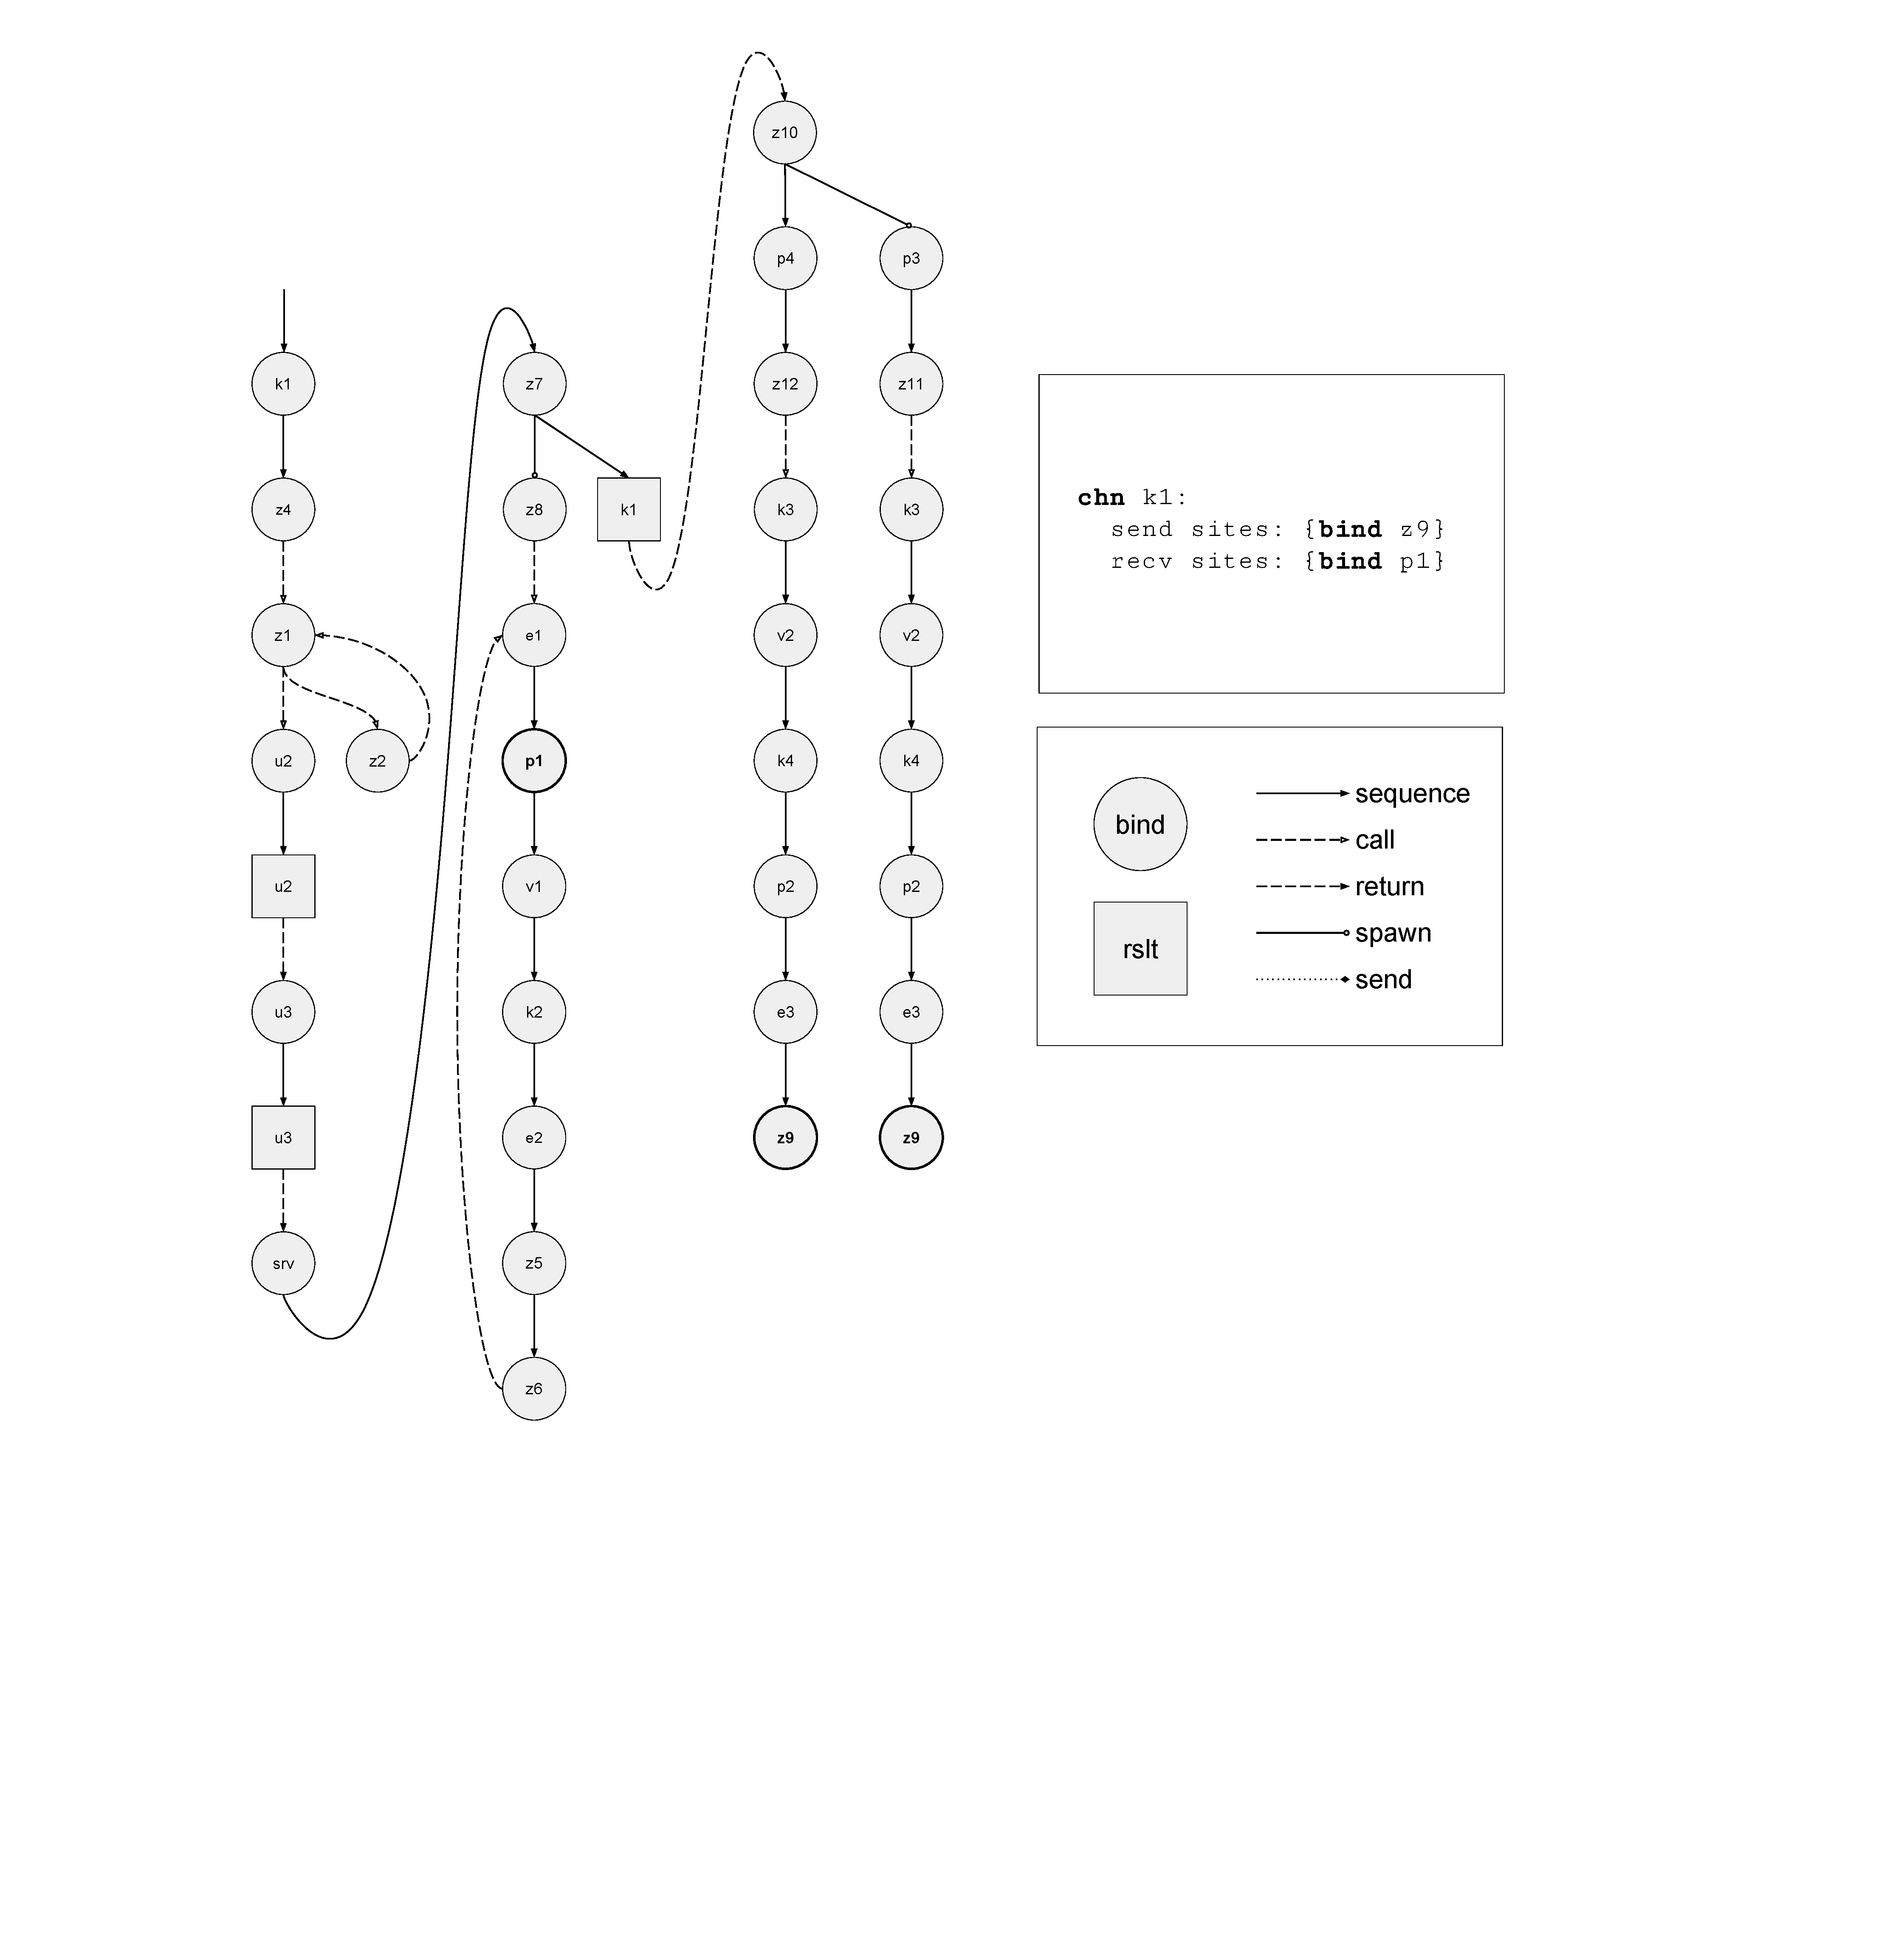
\includegraphics[width=0.9\textwidth]{cml-graph-k1.pdf}

The following diagram illustrates the graph of the server example,
containing only live flows for channel \lstinline{k4}. \

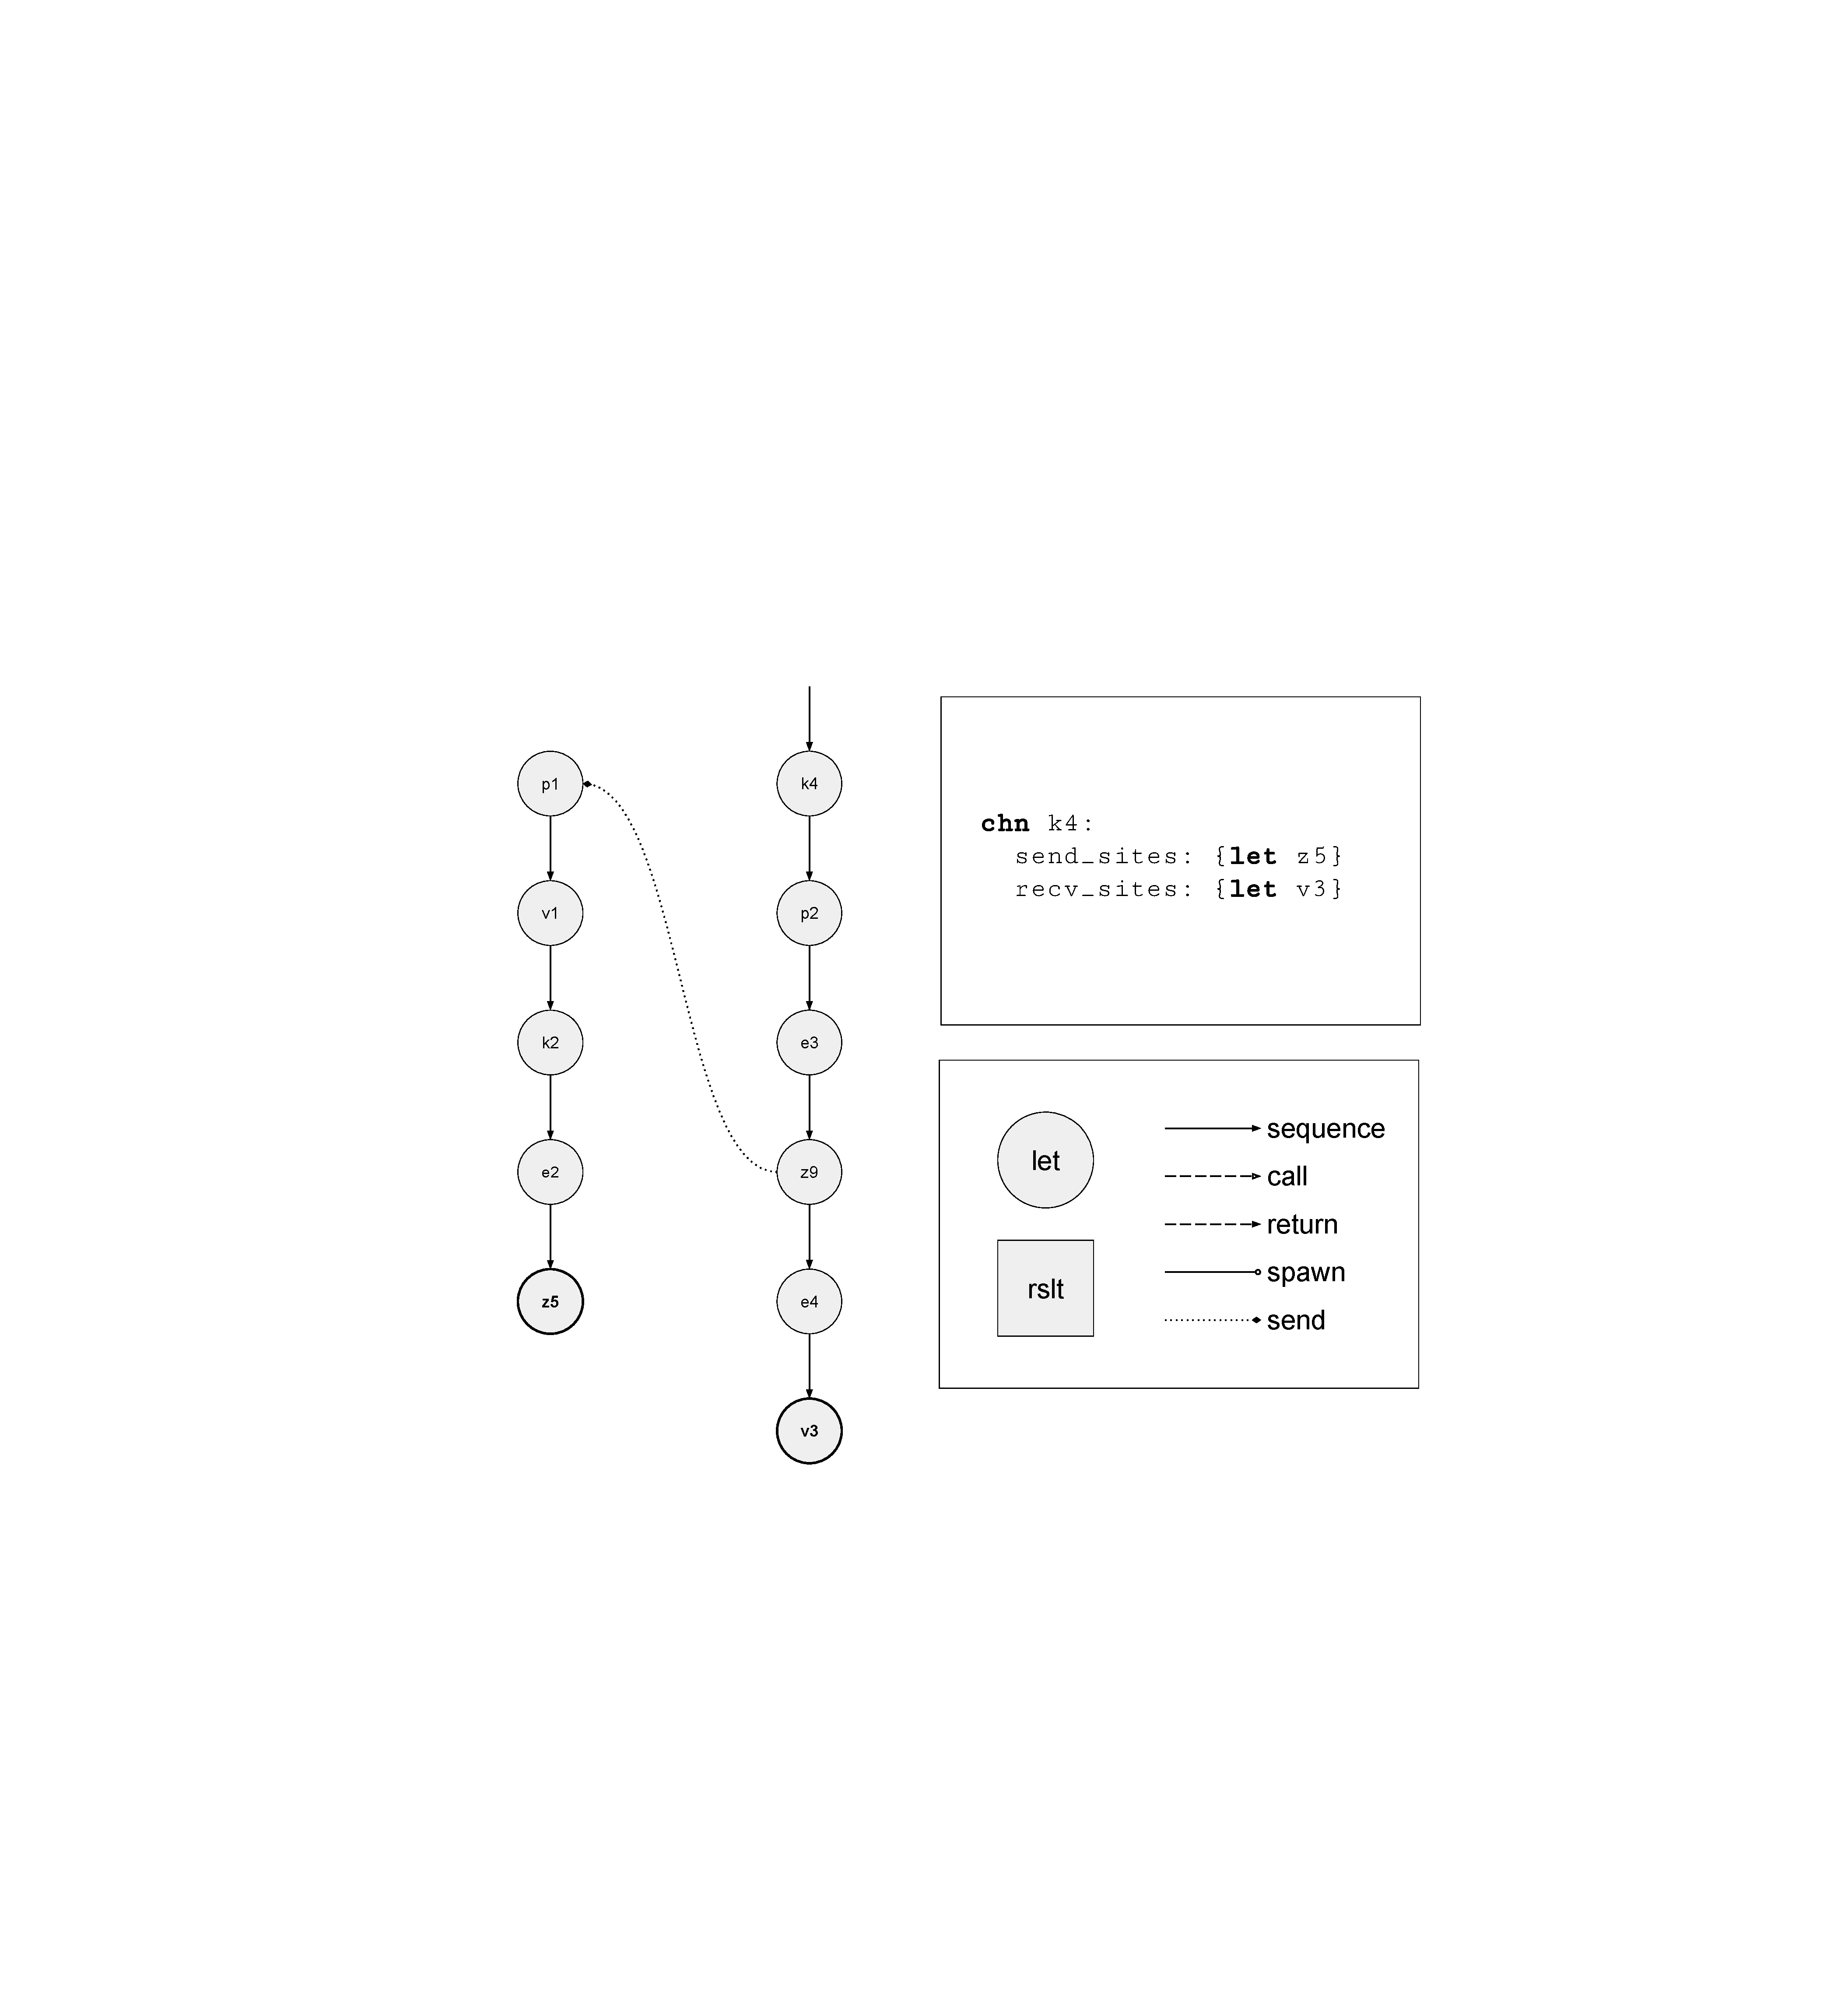
\includegraphics[width=0.7\textwidth]{cml-graph-k4.pdf}

\begin{lstlisting}[language=logic, mathescape]
  predicate staticTraceable:
    static_value_map -> graph -> term_id_map -> term_id_map ->
    termId -> (termId -> bool) -> static_path -> bool where
    $\forall$ isEnd start staticEnv graph entr exit .
      if
        isEnd start
      then
        staticTraceable graph entr exit start isEnd []
   * $\forall$ graph entr exit start middle path isEnd mode. 
      if
        staticTraceable graph entr exit start ($\lambda$ l . l = middle) path, 
        (isEnd end),
        staticLiveFlow graph entr exit (middle, mode, end) 
      then
        staticTraceable graph entr exit start isEnd (path @ [(middle, mode)]
\end{lstlisting}

As with the lower precision analysis, the higher precision analysis relies on recognizing
whether or not two paths can actually occur within in a single run of a program. The static
inclusiveness states which paths might occur within the same run of the program.
In contrast to the analogous definition for the lower precision
alysis, the higher precision definition needs to consider paths containing the
sending mode.  As mentioned earlier, the path from the synchronization on sending to the
synchronization on receiving is necessary to ensure that all uses of a channel are reachable
from the channel's creation identifier.  The singularness means that only one of the two
given paths can occur in a run of program.  The noncompetitveness means that the two
given paths do not compete in any run of a program. 

\begin{lstlisting}[language=logic, mathescape]
  predicate staticInclusive: static_path -> static_path -> bool where
    $\forall$ path1 path2 .
      if
        prefix path1 path2 $\vee$ path2 path1
      then
        staticInclusive path1 path2
  * $\forall$ path n path1 path2 .
      staticInclusive
        (path @ (NBnd n, MSpwn) # path1)
        (path @ (NBnd n, MNxt) # path2)
  * $\forall$ path n path1 path2 .
      staticInclusive
        (path @ (NBnd n, MNxt) # path1)
        (path @ (NBnd n, MSpwn) # path2)
  * $\forall$ path n path1 path2 .
      staticInclusive
        (path @ (NBnd n, ESend xE) # path1)
        (path @ (NBnd n, MNxt) # path2)
  * $\forall$ path n path1 path2 .
      staticInclusive
        (path @ (NBnd n, MNxt) # path1)
        (path @ (NBnd n, ESend xE) # path2)

  predicate singular: static_path -> static_path -> bool where
    $\forall$ path .
      singular path path
  * $\forall$ path1 path2 .
      if
        not (staticInclusive path1 path2)
      then
        singular path1 path2

  predicate noncompetitive: static_path -> static_path -> bool where
    $\forall$ path1 path2 . 
      if
        ordered path1 path2
      then
        noncompetitive path1 path2
  * $\forall$ path1 path2 .
      if
        not (staticInclusive path1 path2)
      then
        noncompetitive path1 path2
  \end{lstlisting}

The communication classifications are described using the liveness properties, but
are otherwise similar to the lower precision classifications.

\begin{lstlisting}[language=logic, mathescape]
  predicate staticOneShot: static_value_map -> term -> name -> bool where
    $\forall$ graph entr exit n$_c$ staticEnv t . 
      if
        forEveryTwo
          (staticTraceable graph entr exit
            (NBnd n$_c$) (staticSendId staticEnv t n$_c$))
          singular, 
        staticLiveChan staticEnv entr exit n$_c$ t, 
        staticFlowsAccept staticEnv graph t
      then
        staticOneShot V t n$_c$)

  predicate staticOneToOne: static_value_map -> term -> name -> bool where
    $\forall$ graph entr exit n$_c$ staticEnv t .
      if
        forEveryTwo
          (staticTraceable graph
            entr exit (NBnd n$_c$) (staticSendId staticEnv t n$_c$))
          noncompetitive, 
        forEveryTwo
          (staticTraceable graph
            entr exit (NBnd n$_c$) (staticRecvId staticEnv t n$_c$))
          noncompetitive,
          staticLiveChan staticEnv entr exit n$_c$ t,
          staticFlowsAccept staticEnv graph t
      then
        staticOneToOne staticEnv t n$_c$)

  predicate staticOneToMany: static_value_map -> term -> name -> bool where
    $\forall$ graph entr exit n$_c$ staticEnv t .
      if
        forEveryTwo
          (staticTraceable graph
            entr exit (NBnd n$_c$) (staticSendId staticEnv t n$_c$))
          noncompetitive,
        staticLiveChan staticEnv entr exit n$_c$ t,
        staticFlowsAccept staticEnv graph t
      then
        staticOneToMany staticEnv t n$_c$)

  predicate staticManyToOne: static_value_map -> term -> name -> bool where
    $\forall$ graph entr exit n$_c$ staticEnv t .
      if
        forEveryTwo
          (staticTraceable graph
            entr exit (NBnd n$_c$) (staticRecvId staticEnv t n$_c$))
          noncompetitive, 
        staticLiveChan staticEnv entr exit n$_c$ t,
        staticFlowsAccept staticEnv graph t
      then
        staticManyToOne staticEnv t n$_c$)
  \end{lstlisting}


\subsection{Higher Precision Soundness Proof Strategy}
To prove soundness of the communication classification, it should be possible to use
previous techniques of generalizing propositions over pools and other semantic components,
along with finding equivalent representations of propositions that vary in the inductive
subcomponent. One thing that will make carrying out the formal proof particularly tricky is
that dynamic paths in the dynamic semantics need to correspond to static paths from
the trimmed graphs, which might also contain sending flows,
instead of the dynamic paths spawning flows.
The correspondence between these dynamic paths and static paths
is not bijective, as it is for the lower precision analysis. However, finding a satisfactory
correspondence for each dynamic and static path is critical for proving soundness.

Essentially, it will be necessary to show that static
properties that hold for some static path are preserved for corresponding dyamic paths. 
However, in the higher precision analysis these paths correspond modulo the channel of interest.
Let's outline the derivation of soundness of one-shot classification.

\begin{lstlisting}[language=logic, mathescape]
  theorem staticOneShotSound:
  $\forall$ t$_0$ pool comm staticEnv staticComm n$_c$ path$_c$ . 
    if
      star dynamicEval [[] -> (Stt t$_0$ [->] []] {} pool comm,
      staticEval staticEnv staticComm t$_0$,
      staticOneShot staticEnv t$_0$ n$_c$
    then 
      oneShot pool (Chan path$_c$ n$_c$)
\end{lstlisting}

The theorem for soundness of one-shot classification depends on
correlating dynamic paths with static paths.

\begin{lstlisting}[language=logic, mathescape]
  predicate pathsCorrespond: dynamic_path -> static_path -> bool where
    pathsCorrespond [] []
  * $\forall$ path staticPath n .
      if
        pathsCorrespond path staticPath
      then
        pathsCorrespond
          (path @ [DNxt n])
          (staticPath @ [(NBnd n, MNxt)])
  * $\forall$ path staticPath n .
      if
        pathsCorrespond path staticPath
      then
        pathsCorrespond
          (path @ [DSpwn n])
          (staticPath @ [(NBnd n, MSpwn)])
  * $\forall$ path staticPath n .
      if
        pathsCorrespond path staticPath
      then
        pathsCorrespond
          (path @ [DCll n])
          (staticPath @ [(NBnd n, MCll)])
  * $\forall$ path staticPath n .
      if
        pathsCorrespond path staticPath
      then
        pathsCorrespond
          (path @ [DRtn n])
        (staticPath @ [(NRslt n, MRtn)])

  predicate pathsCorrespondModChan:
    pool -> communication -> chan -> dynamic_path -> static_path -> bool where
    $\forall$ pool path$_c$ n$_c$ path$_{sfx}$ stt staticPath comm .
      if
        pool (path$_c$ @ (DNxt n$_c$) # path$_{sfx}$) = Some stt,
        pathsCorrespond ((DNxt n$_c$) # path$_{sfx}$) staticPath
      then
        pathsCorrespondModChan
          (pool, comm) (Chan path$_c$ n$_c$)
          (path$_c$ @ (DNxt n$_c$) # path$_{sfx}$) staticPath
  * $\forall$ pool path$_r$ n$_r$ path$_{sfx}$ stt  path$_s$ n$_s$ n$_{se}$ t$_{sy}$ env$_{sy}$ stack$_{sy}$
      n$_{re}$ t$_{ry}$ env$_{ry}$ stack$_{ry}$ c$_c$ comm c staticPath$_{re}$ staticPath$_{sfx}$ . 
      if
        pool (path$_r$ @ (DNxt n$_r$) # path$_{sfx}$) = Some stt, 
        pool path$_s$ = Some (Stt (Bind n$_s$ (Sync n$_{se}$) t$_{sy}$) env$_{sy}$ stack$_{sy}$),
        pool path$_r$ = Some (Stt (Bind n$_r$ (Sync n$_{re}$) t$_{ry}$) env$_{ry}$ stack$_{ry}$),
        {(path$_s$, c$_c$, path$_r$)} $\subseteq$ comm, 
        dynamicBuiltOnChanVar env$_{ry}$ c n$_r$, 
        pathsCorrespondModChan pool comm c path$_s$ staticPath$_{pfx}$,
        pathsCorrespond path$_{sfx}$ staticPath$_{sfx}$
      then
        pathsCorrespondModChan pool comm c
          (path$_r$ @ (DNxt n$_r$) # path$_{sfx}$)
          (staticPath$_{pfx}$ @ (NBnd n$_s$, ESend n$_{se}$)
            # (NBnd n$_r$, MNxt) # staticPath$_{sfx}$)
\end{lstlisting}

Additionally the soundness theorem follows from the completeness of static traceability,
the completeness of static inclusiveness, and the completeness of a sending identifier classification. 
The reasoning about the sending identifier is identical to that of the lower precision analysis, but
the reasoning for the former two is significantly more complicated and not yet completed.
The complication arises from the
correlation between dynamic paths and static paths.  The proofs depend on finding a static 
path that depends on a given dynamic path. In the lower precision analysis the
correlation was straightforward. There was only one possible static path to choose for it
to correlate with the given dynamic path. In the higher precision analysis, the relationship
between the two kinds of paths is not so simple, and finding a description of the static path
that correlates with the dynamic path is much more challenging.

\begin{lstlisting}[language=logic, mathescape]
  predicate pathsCorrespond: dynamic_path -> static_path -> bool where
    pathsCorrespond [] []
  * $\forall$ path staticPath n .
      if
        pathsCorrespond path staticPath
      then
        pathsCorrespond
          (path @ [DNxt n])
          (staticPath @ [(NBnd n, MNxt)])
  * $\forall$ path staticPath n .
      if
        pathsCorrespond path staticPath
      then
        pathsCorrespond
          (path @ [DSpwn n])
          (staticPath @ [(NBnd n, MSpwn)])
  * $\forall$ path staticPath n .
      if
        pathsCorrespond path staticPath
      then
        pathsCorrespond
          (path @ [DCll n])
        (staticPath @ [(NBnd n, MCll)])
  * $\forall$ path staticPath n .
      if
        pathsCorrespond path staticPath
      then
        pathsCorrespond
          (path @ [DRtn n])
        (staticPath @ [(NRslt n, MRtn)])

  predicate pathsCorrespondModChan:
    pool -> communication -> chan -> dynamic_path -> static_path -> bool where
    $\forall$ pool path$_c$ n$_c$ path$_{sfx}$ stt staticPath comm .
      if
        pool (path$_c$ @ (DNxt n$_c$) # path$_{sfx}$) = Some stt,
        pathsCorrespond ((DNxt n$_c$) # path$_{sfx}$) staticPath
      then
        pathsCorrespondModChan
          (pool, comm) (Chan path$_c$ n$_c$)
          (path$_c$ @ (DNxt n$_c$) # path$_{sfx}$) staticPath
  * $\forall$ pool path$_r$ n$_r$ path$_{sfx}$ stt path$_s$ n$_s$ n$_{se}$ t$_{sy}$ env$_{sy}$ stack$_{sy}$
      n$_{re}$ t$_{ry}$ env$_{ry}$ stack$_{ry}$ c$_c$ comm c staticPath$_{re}$ staticPath$_{sfx}$ . 
      if
        pool (path$_r$ @ (DNxt n$_r$) # path$_{sfx}$) = Some stt, 
        pool path$_s$ = Some (Stt (Bind n$_s$ (Sync n$_{se}$) t$_{sy}$) env$_{sy}$ stack$_{sy}$),
        pool path$_r$ = Some (Stt (Bind n$_r$ (Sync n$_{re}$) t$_{ry}$) env$_{ry}$ stack$_{ry}$),
        {(path$_s$, c$_c$, path$_r$)} $\subseteq$ comm, 
        dynamicBuiltOnChanVar env$_{ry}$ c n$_r$, 
        pathsCorrespondModChan pool comm c path$_s$ staticPath$_{pfx}$,
        pathsCorrespond path$_{sfx}$ staticPath$_{sfx}$
      then
        pathsCorrespondModChan pool comm c
          (path$_r$ @ (DNxt n$_r$) # path$_{sfx}$)
          (staticPath$_{pfx}$ @ (NBnd n$_s$, ESend n$_{se}$)
            # (NBnd n$_r$, MNxt) # staticPath$_{sfx}$)

  lemma staticTraceableSound:
    $\forall$ t$_0$ pool comm path n c t' env stack staticEnv staticComm
      entr exit n$_c$ graph isEnd path$_c$  . 
      if
        star dynamicEval [[] -> (Stt t$_0$ [->] [])] {} pool comm,
        pool path = Some (Stt (Bind n c t') env stack),
        staticEval staticEnv staticComm t$_0$,
        staticLiveChan staticEnv entr exit n$_c$ t$_0$,
        staticFlowsAccept staticEnv graph t$_0$, 
        isEnd (NBnd n)
      then
        (exists staticPath . 
          pathsCorrespondModChan pool comm (Chan path$_c$ n$_c$) path staticPath, 
          staticTraceable graph entr exit (NBnd n$_c$) isEnd staticPath)

  lemma staticInclusiveSound:
    $\forall$ t$_0$ pool comm staticEnv entr exit n$_c$ graph staticComm
      path1 stt1 path$_c$ staticPath1 path2 stt2 staticPath2 .
      if
        star dynamicEval [[] -> (Stt t$_0$ [->] [])] {} pool comm, 
        staticLiveChan staticEnv entr exit n$_c$ t$_0$, 
        staticFlowsAccept staticEnv graph t$_0$, 
        staticEval staticEnv staticComm t$_0$, 
        pool path1 = Some stt1, 
        pathsCorrespondModChan pool comm (Chan path$_c$ n$_c$) path1 staticPath1, 
        staticTraceable graph entr exit
          (NBnd n$_c$) (staticSendId staticEnv t$_0$ n$_c$) staticPath1, 
        pool path2 = Some stt2, 
        pathsCorrespondModChan pool comm (Chan path$_c$ n$_c$) path2 staticPath2, 
        staticTraceable graph entr exit
          (NBnd n$_c$) (staticSendId staticEnv t$_0$ n$_c$) staticPath2
      then
        staticInclusive staticPath1 staticPath2
\end{lstlisting}

  



\section{Related Work}
There has been much research on both dynamic and static analysis of concurrent languages.  
The formal communication classification analysis and soundness proofs in this work are
based on the analysis and proofs of \textit{Specialization of CML message-passing primitives}
by Reppy and Xiao \cite{reppy2007specialization}.
The mechanization of concurrency analyses is prevalent, and mechanization is typically the main
goal when developing the analyses. Examples include type checkers in compilers,
model checking tools for concurrent models, such as Lustre \cite{halbwachs1991synchronous} and Kind \cite{kind},
and also verification libraries in proof assistants, such as Affeldt et al's Coq library \cite{affeldt2008coq}.
These systems can verify certain properties of concurrent programs or models, but they don't
make any guarantees about the analysis itself.
Rather than focus on mechanizing the analysis, this work has focused on
mechanizing the theory of analyses for concurrent languages, i.e. the meta-theory of concurrency.
There have been a number of works on the meta-theory of Concurrent ML,
such as the work of Reppy and Xiao, Nielson et al \cite{nielson$_1$994higher}, Kobayashi et al \cite{kobayashi1995static}, and Gasser et al \cite{gasser1997systematic}.
There has been relatively little work to mechanize theories of Concurrent ML; however,
there has been much work in the mechanization of the theories of $\pi$-calculus
\cite{milner1999communicating}, such as the work by Gay \cite{gay2001framework} and Melham \cite{melham1994mechanized}. 

\section{Future Work}
The formal syntax, semantics, and communication analysis of this work form the basis of
a framework for studying concurrency functions, synchronization mechanisms, and their
applications. These language features enable the construction of reactive programs, which
have separation of parts that are conceptually distinct, yet still depend on each
other.

This work has kicked off the framework with a formal communication analysis that has practical
applications in aiding optimizations for parallel computation. In the future, additional
analyses could be built on the existing semantics, in order to verify the correctness of language 
extensions or optimizations. Extending the semantics to handle event combinators for choosing
events, sequencencing events, guardining events, among others, would be an important next step.

Concurreny is a double edged sword. Without specification of ordering, programs may
desribe their behavior more clearly or allow parallelism for faster execution. On the other hand,
unspecified orderings may also lead to nondetermistic behavior, which may be not be wanted. 
To gain the benefits of concurrency without its hinderance, the language could be extended
with syntax to identify blocks of code that are required to be deterministic,
along with a corresponding static analysis that checks if such code is actually
deterministic. The determinism analysis could rely on the static communication analysis
to ensure that all syncronized receiving events receive from at most one channel,
that channel is sent on by at most one thread, and that thread is also deterministic.

Other analyses could aid optimizations for incremental computation
\cite{acar2002adaptive}. One possible optimzation could transform a program into one
that checks for altered dependencies and only recomputes the data that depends on altered dependencies.

\newpage

\bibliography{refs}
\bibliographystyle{plain}


\end{document}
